%%%%%%%%%%%%%%%%%%%%%%%%%%%%%%%%%%%%%%%%%%%%%%%%%%%%%%%%%%%%%%%%%
\chapter{EXPERIMENTAL SETUP AND METHODOLOGY}\label{Ch:Ch4_expsetup}
%%%%%%%%%%%%%%%%%%%%%%%%%%%%%%%%%%%%%%%%%%%%%%%%%%%%%%%%%%%%%%%%%
Experiments were performed in the vacuum chamber at the BUSTLab of Bogazici University. The laboratory contains a vacuum chamber, AC and DC power supplies, network matching circuits, propellant container tanks, propellant flow lines and flow controller. Ion beam charge density and divergence is measured by a Faraday cup which is in-house built by members of BUSTLab\cite{yildiz2019plume}. By measuring the beam charge density deductions about produced thrust levels can be made. \\
Majority of experimental setup was manually operated. Ion beam measurement system was controlled by LabVIEW software. In this chapter experimental setup and its elements will be explained. Experimental procedures and attempts at operating the thruster will be provided. 

\section{Experimental Setup}
\newpage
\subsection{Vacuum Chamber}
All experiments were performed in a custom built Kurt J. Lesker brand vacuum chamber shown in figure \ref{fig:bustlabchamber}. It has a diameter of 1.5 meters and lenght of 2.7 meters. It is primarily used to perform experiments with electric propulsion systems that use Argon or Xenon propellant. \\
\begin{figure}[ht]
    \centering
    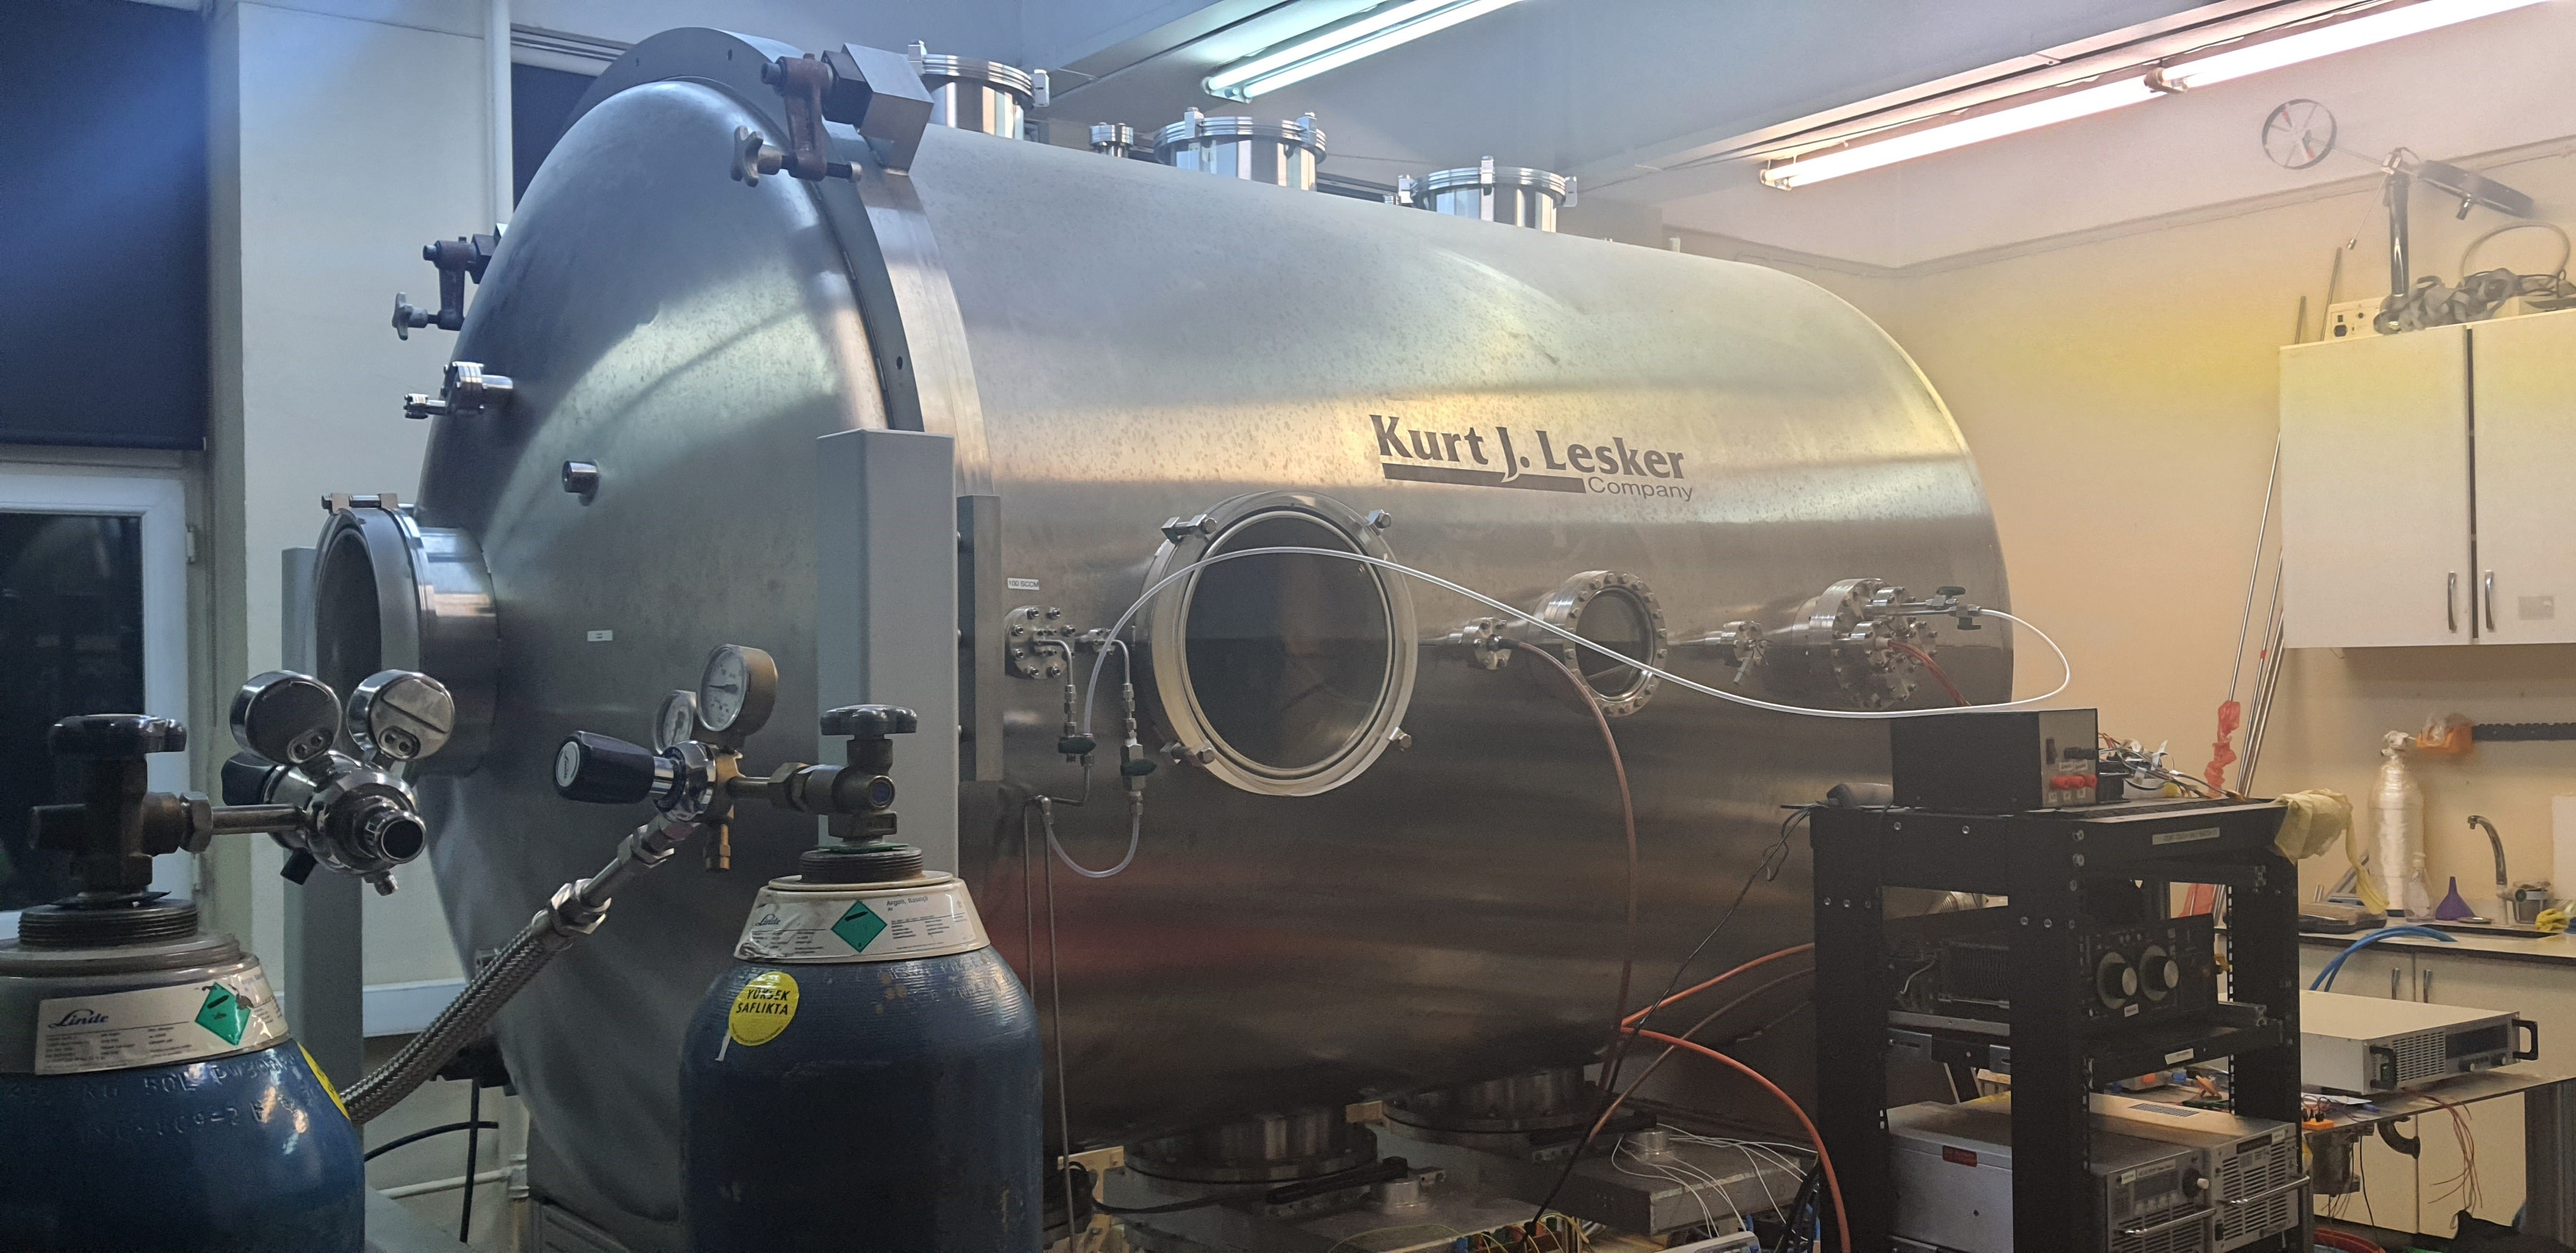
\includegraphics[scale=0.1]{fig/bustlabchamber.jpg}
    \caption{BUSTLab vacuum chamber}
    \label{fig:bustlabchamber}
\end{figure}

The vacuum chamber can achieve high vacuum levels up to $10^{-8}$ torrs thanks to a mechanical and cryogenic pumps. This vacuum level is akin to low earth orbit vacuum levels which ranges between $10^{-7}$ to $10^{-9}$ torrs\cite{Horneck2011}. Vacuum chamber can sustain very low pressure levels even when a thruster is operating in chamber during which a propellant is continuously pumped into the chamber. 

% \begin{figure}[ht]
%     \centering
%     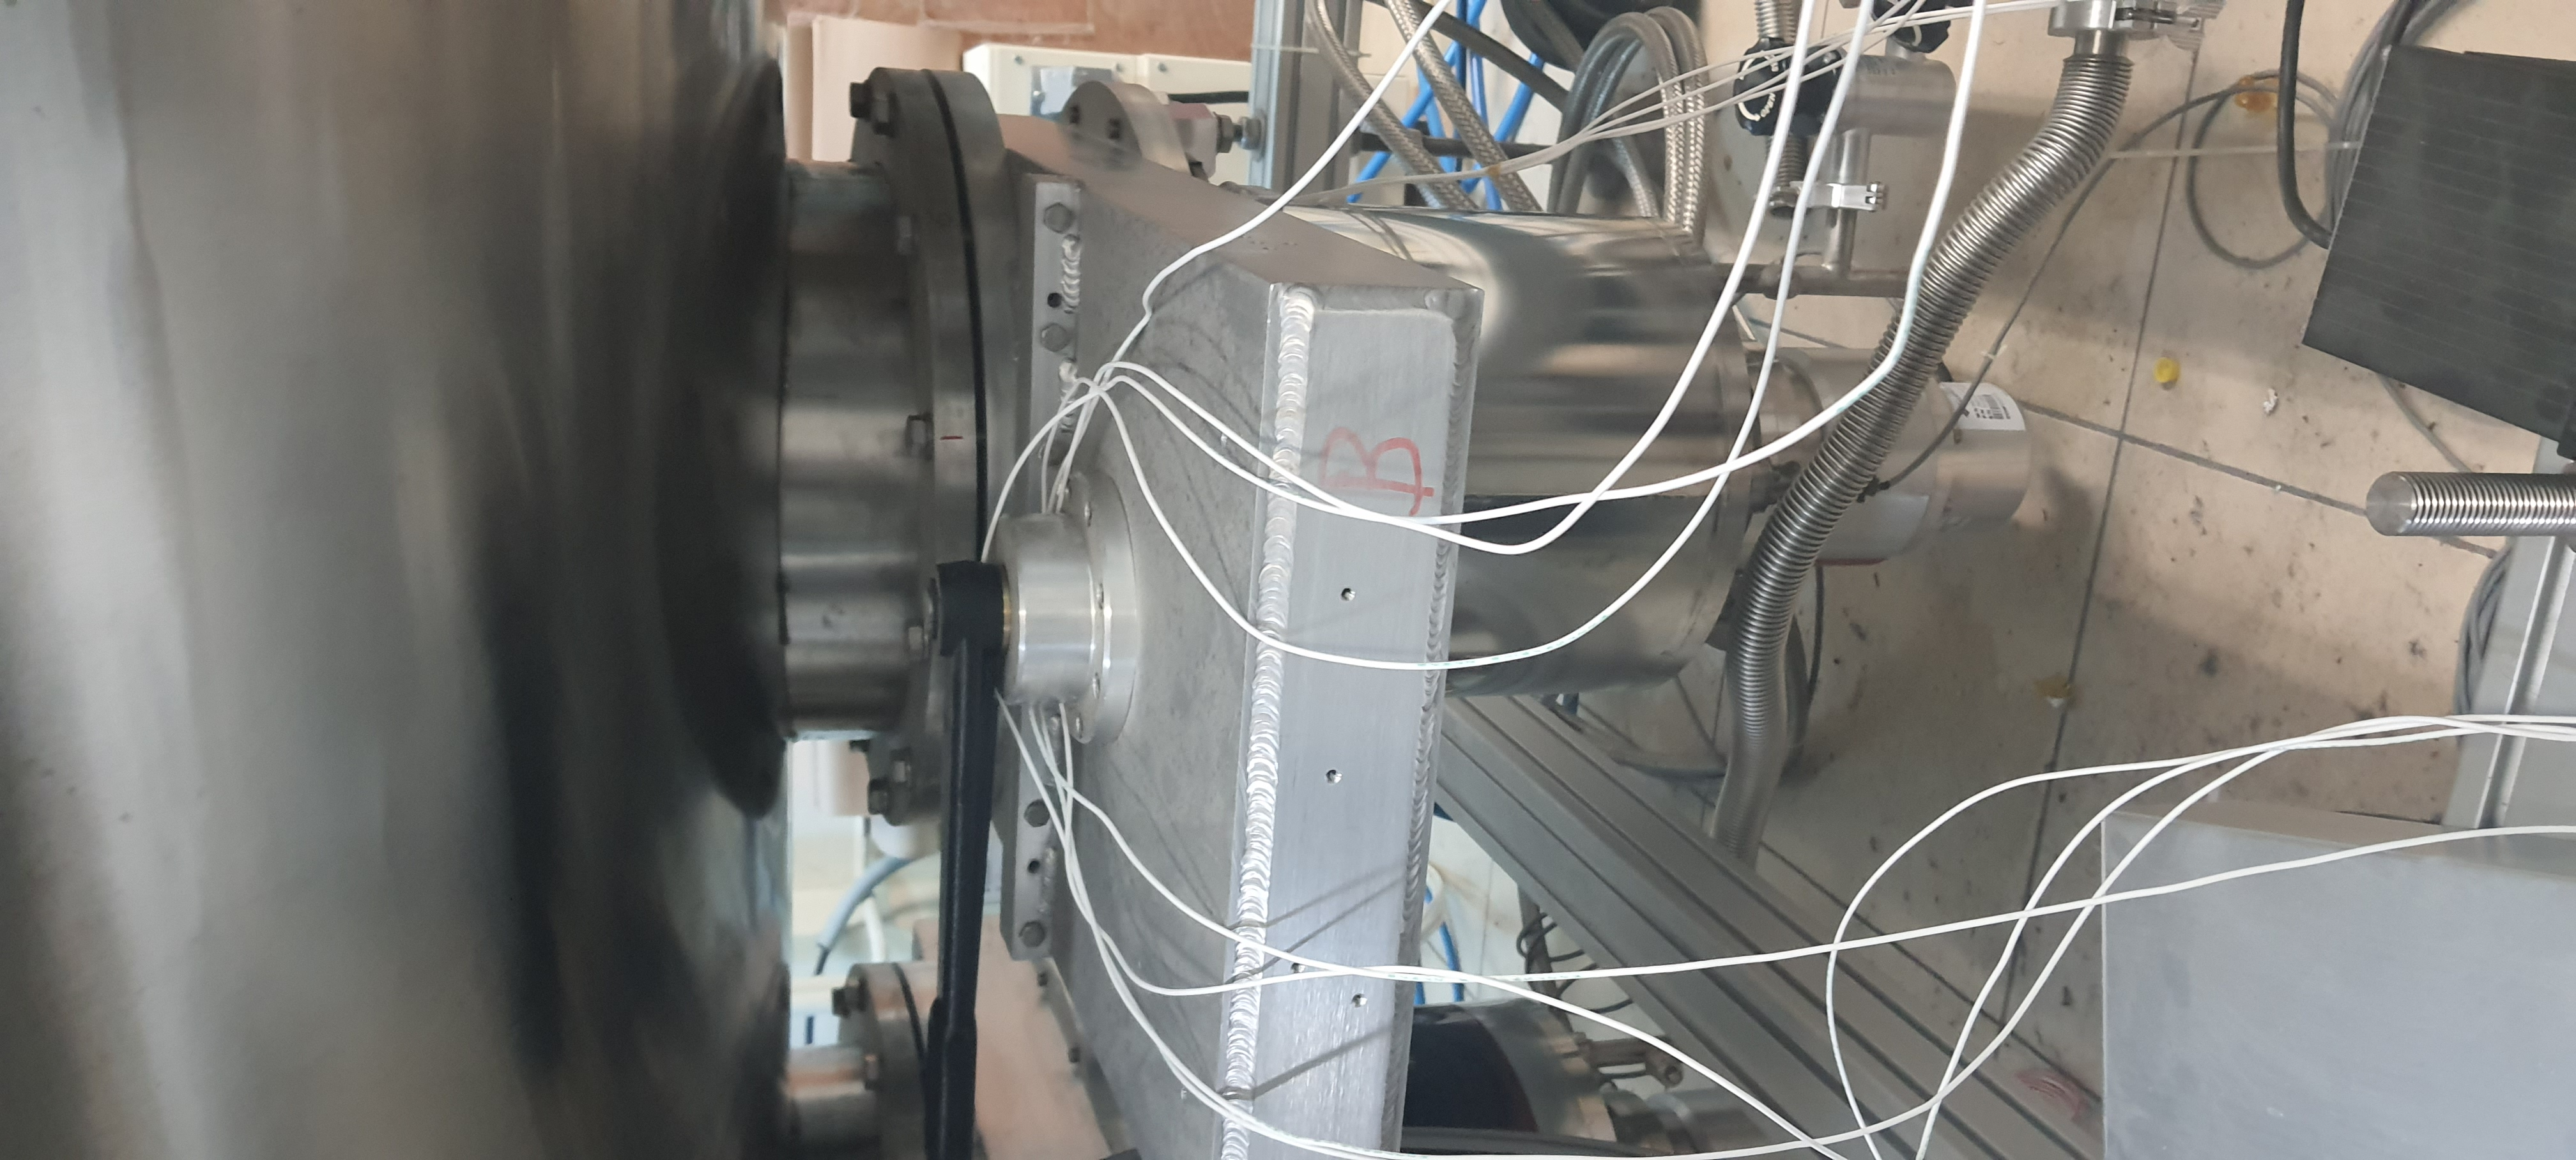
\includegraphics[scale=0.075]{fig/cryopump.jpg}
%     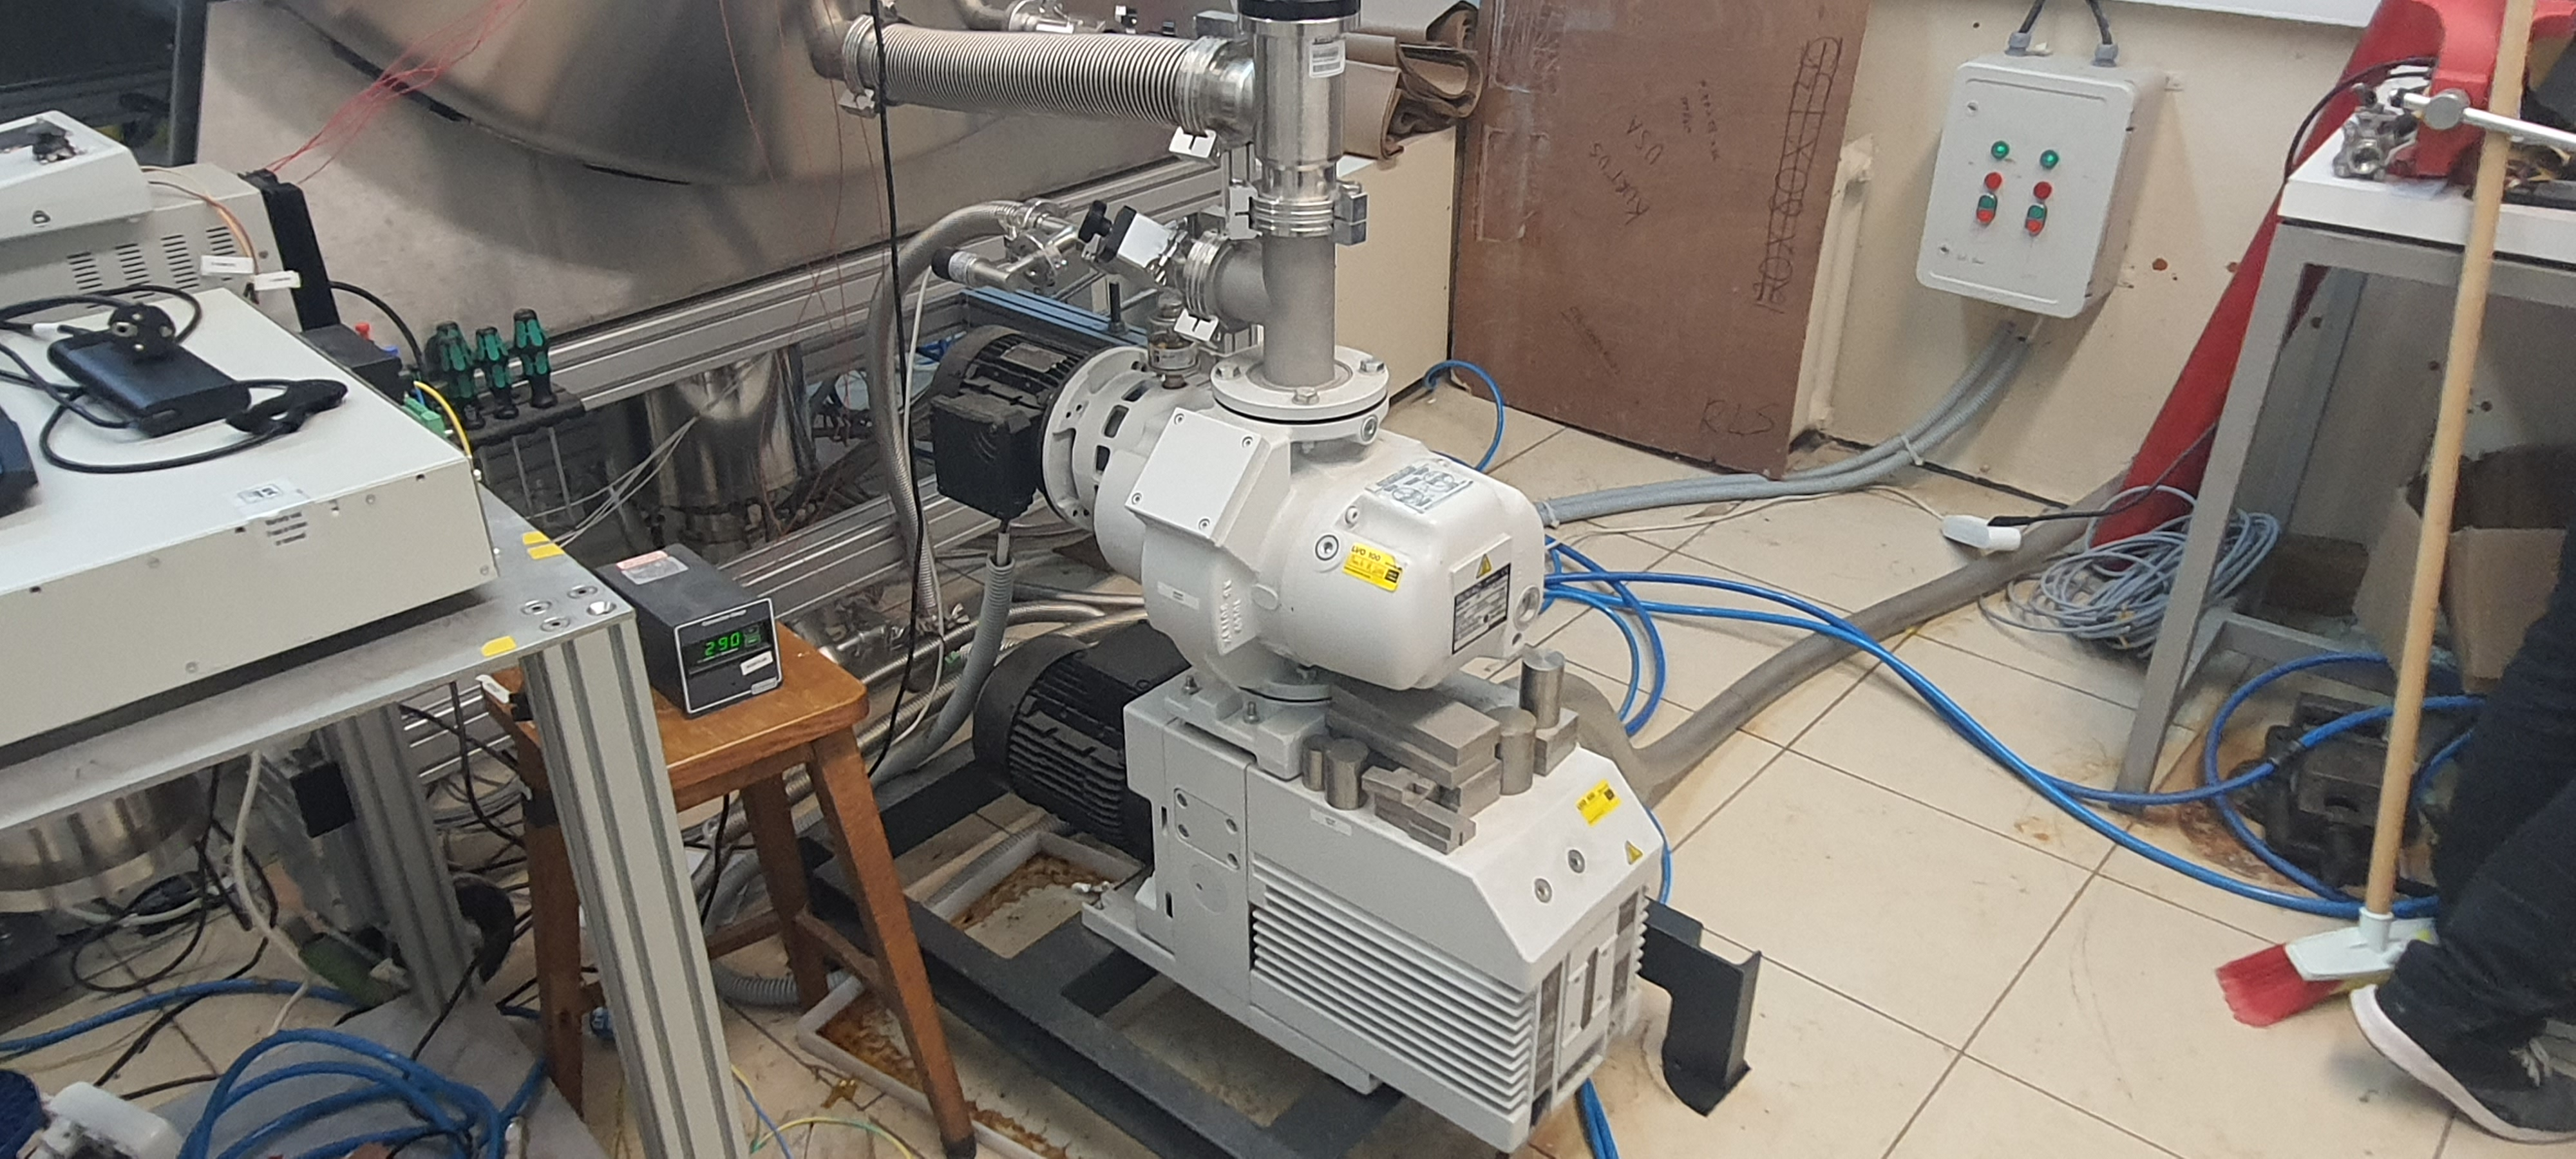
\includegraphics[scale=0.05]{fig/mechanicalpump.jpg}
%     \caption{Cryopump and mechanical pump}
%     \label{fig:bustpump}
% \end{figure}
\newpage
Thrust chamber allows access to the interior through feedthroughs. There are numerous feedthroughs with different sizes and purposes. One of them is used to connect the RF line from the signal source to thruster. Two feedthroughs are used to connect the gas feed. Several feedthroughs are used to connect the DC power lines. 

\begin{figure}[ht]
    \centering
    \includegraphics[height=5cm]{fig/dcfeedout.jpg}
    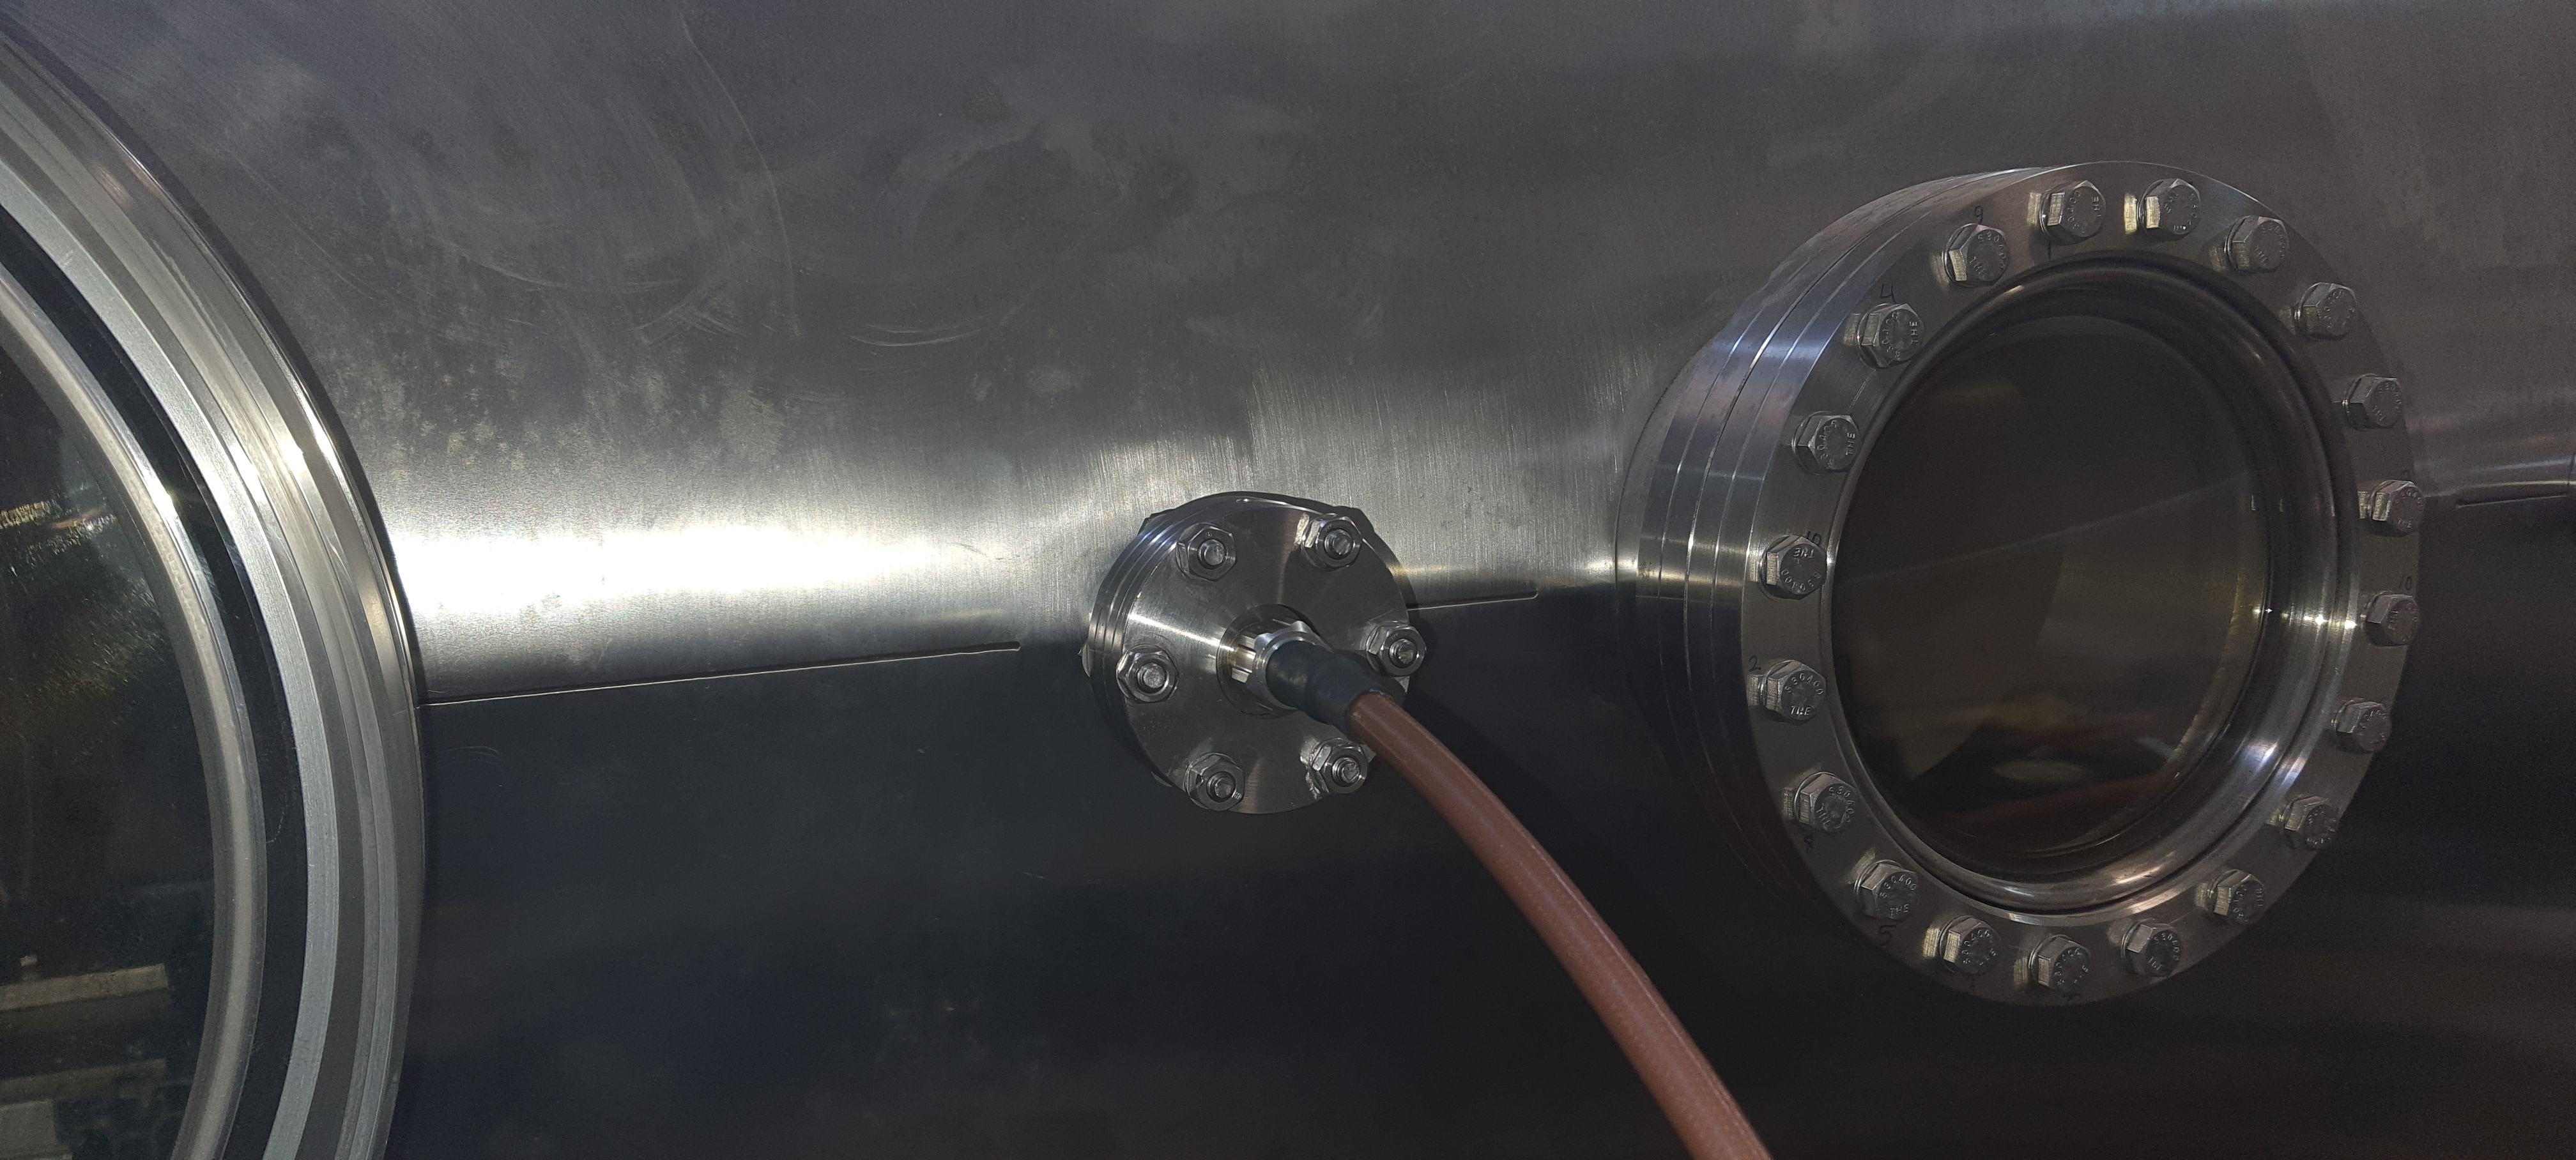
\includegraphics[height=5cm]{fig/RFfeedout.jpg}
    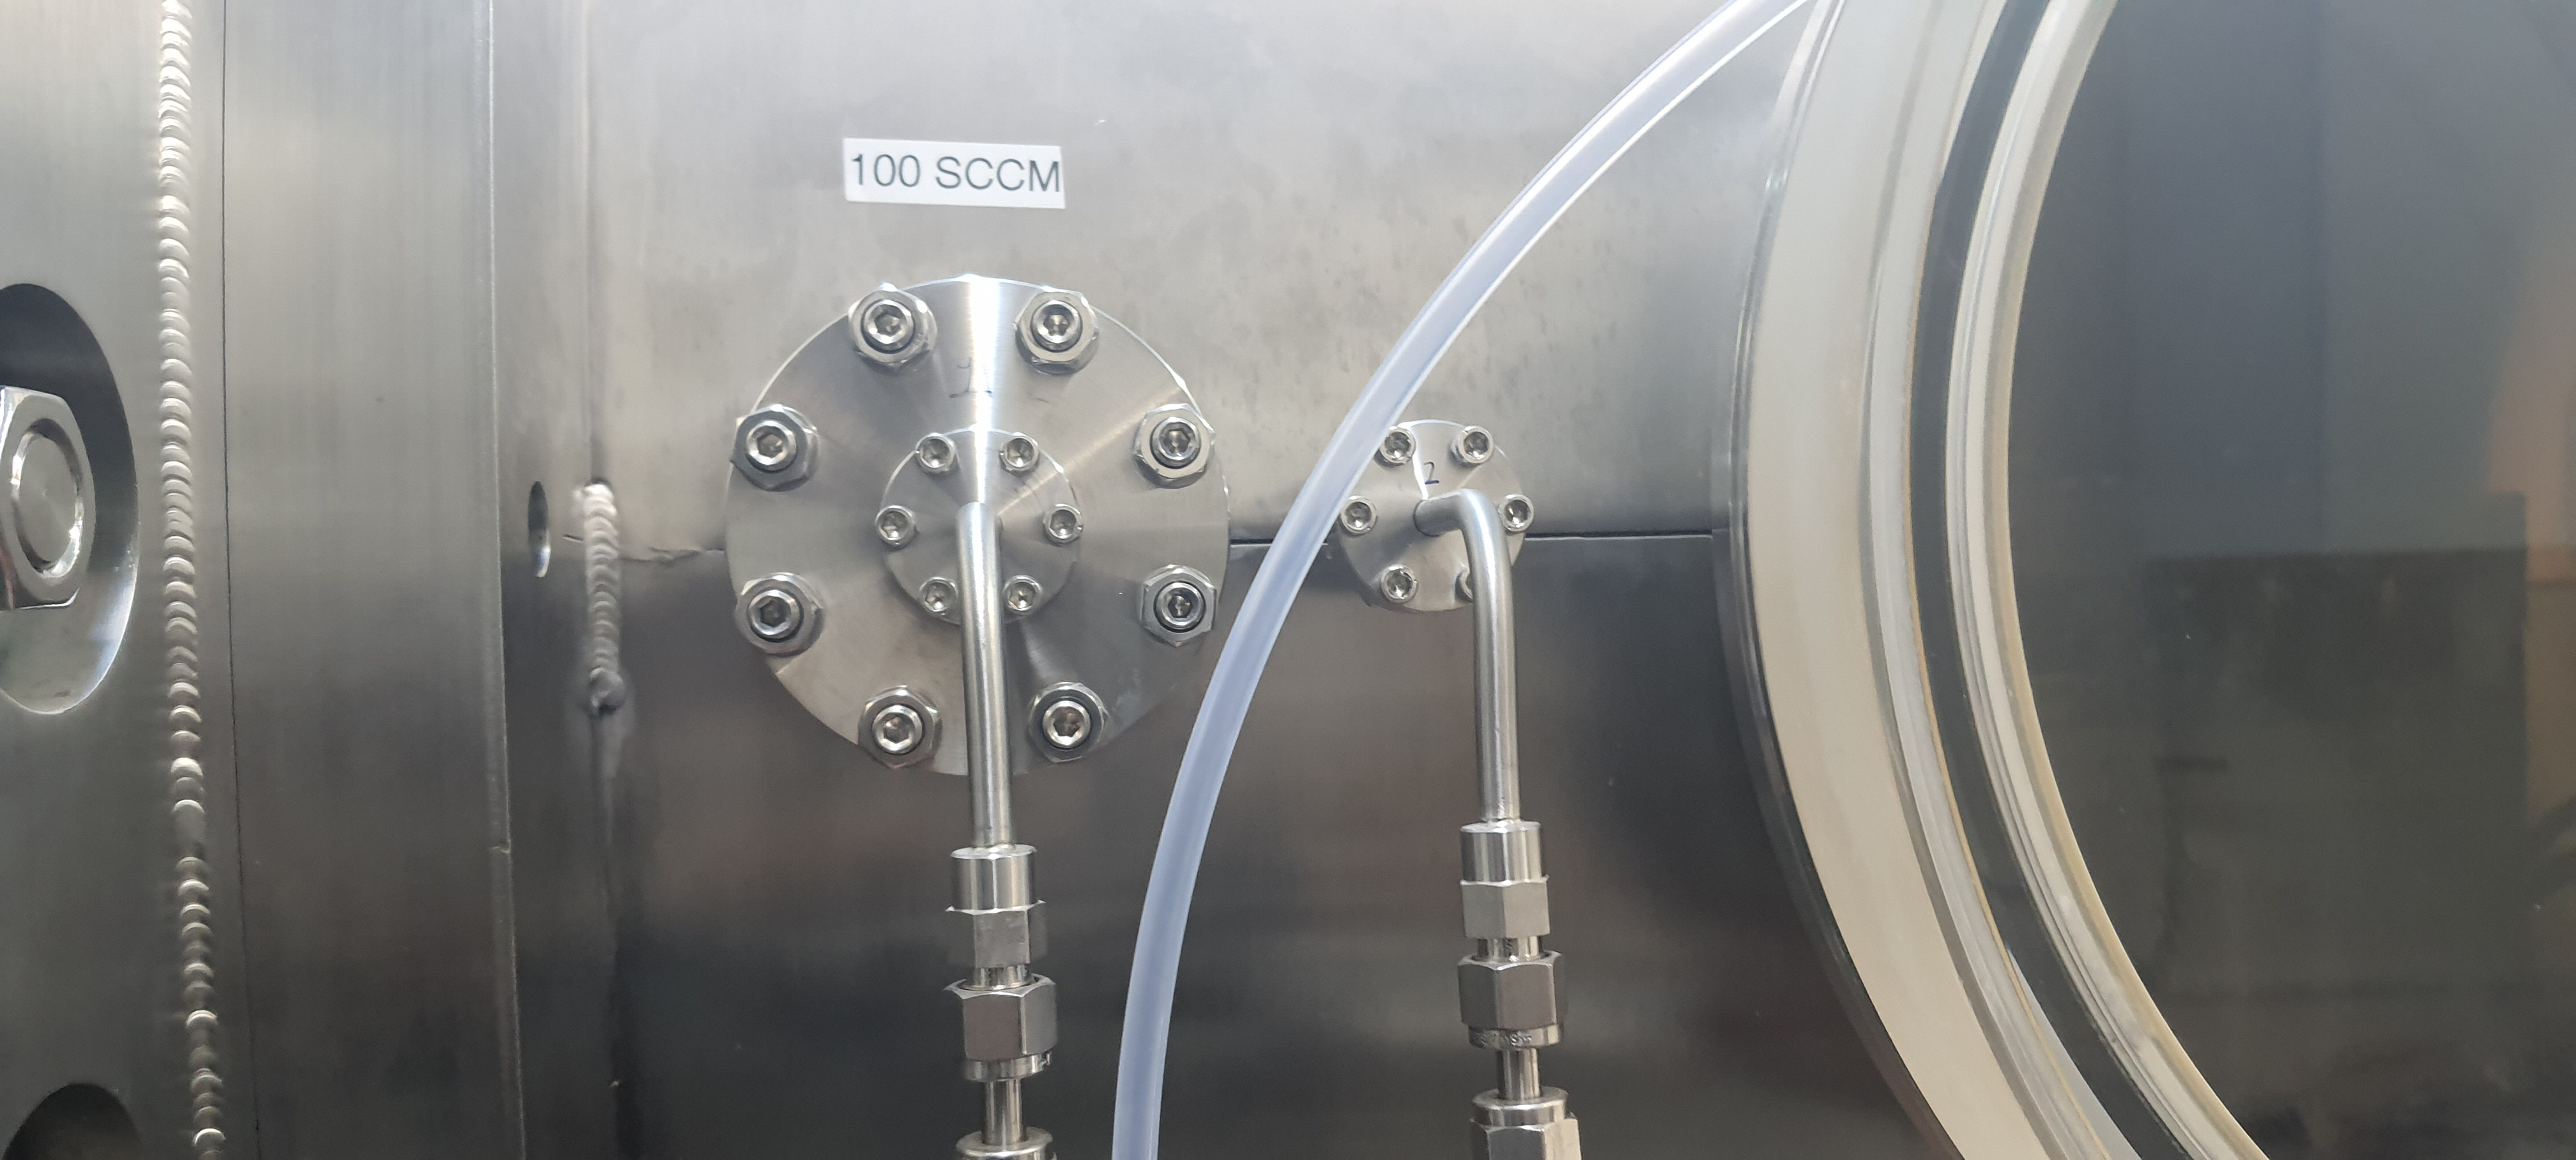
\includegraphics[height=5cm]{fig/gasfeedout.jpg}
    \caption{From top to bottom DC, RF and propellant feedthroughs}
    \label{fig:vacuumfeed}
\end{figure}
\newpage
\subsection{RF Power Supply}
RF power source is AG1213W type RF generator shown in figure \ref{fig:rfpowersup}. It can generate signals with up to 1200W of power. It outputs constant 13.56MHz frequency. It is suitable for industrial, scientific and medical applications.

\begin{figure}[ht]
    \centering
    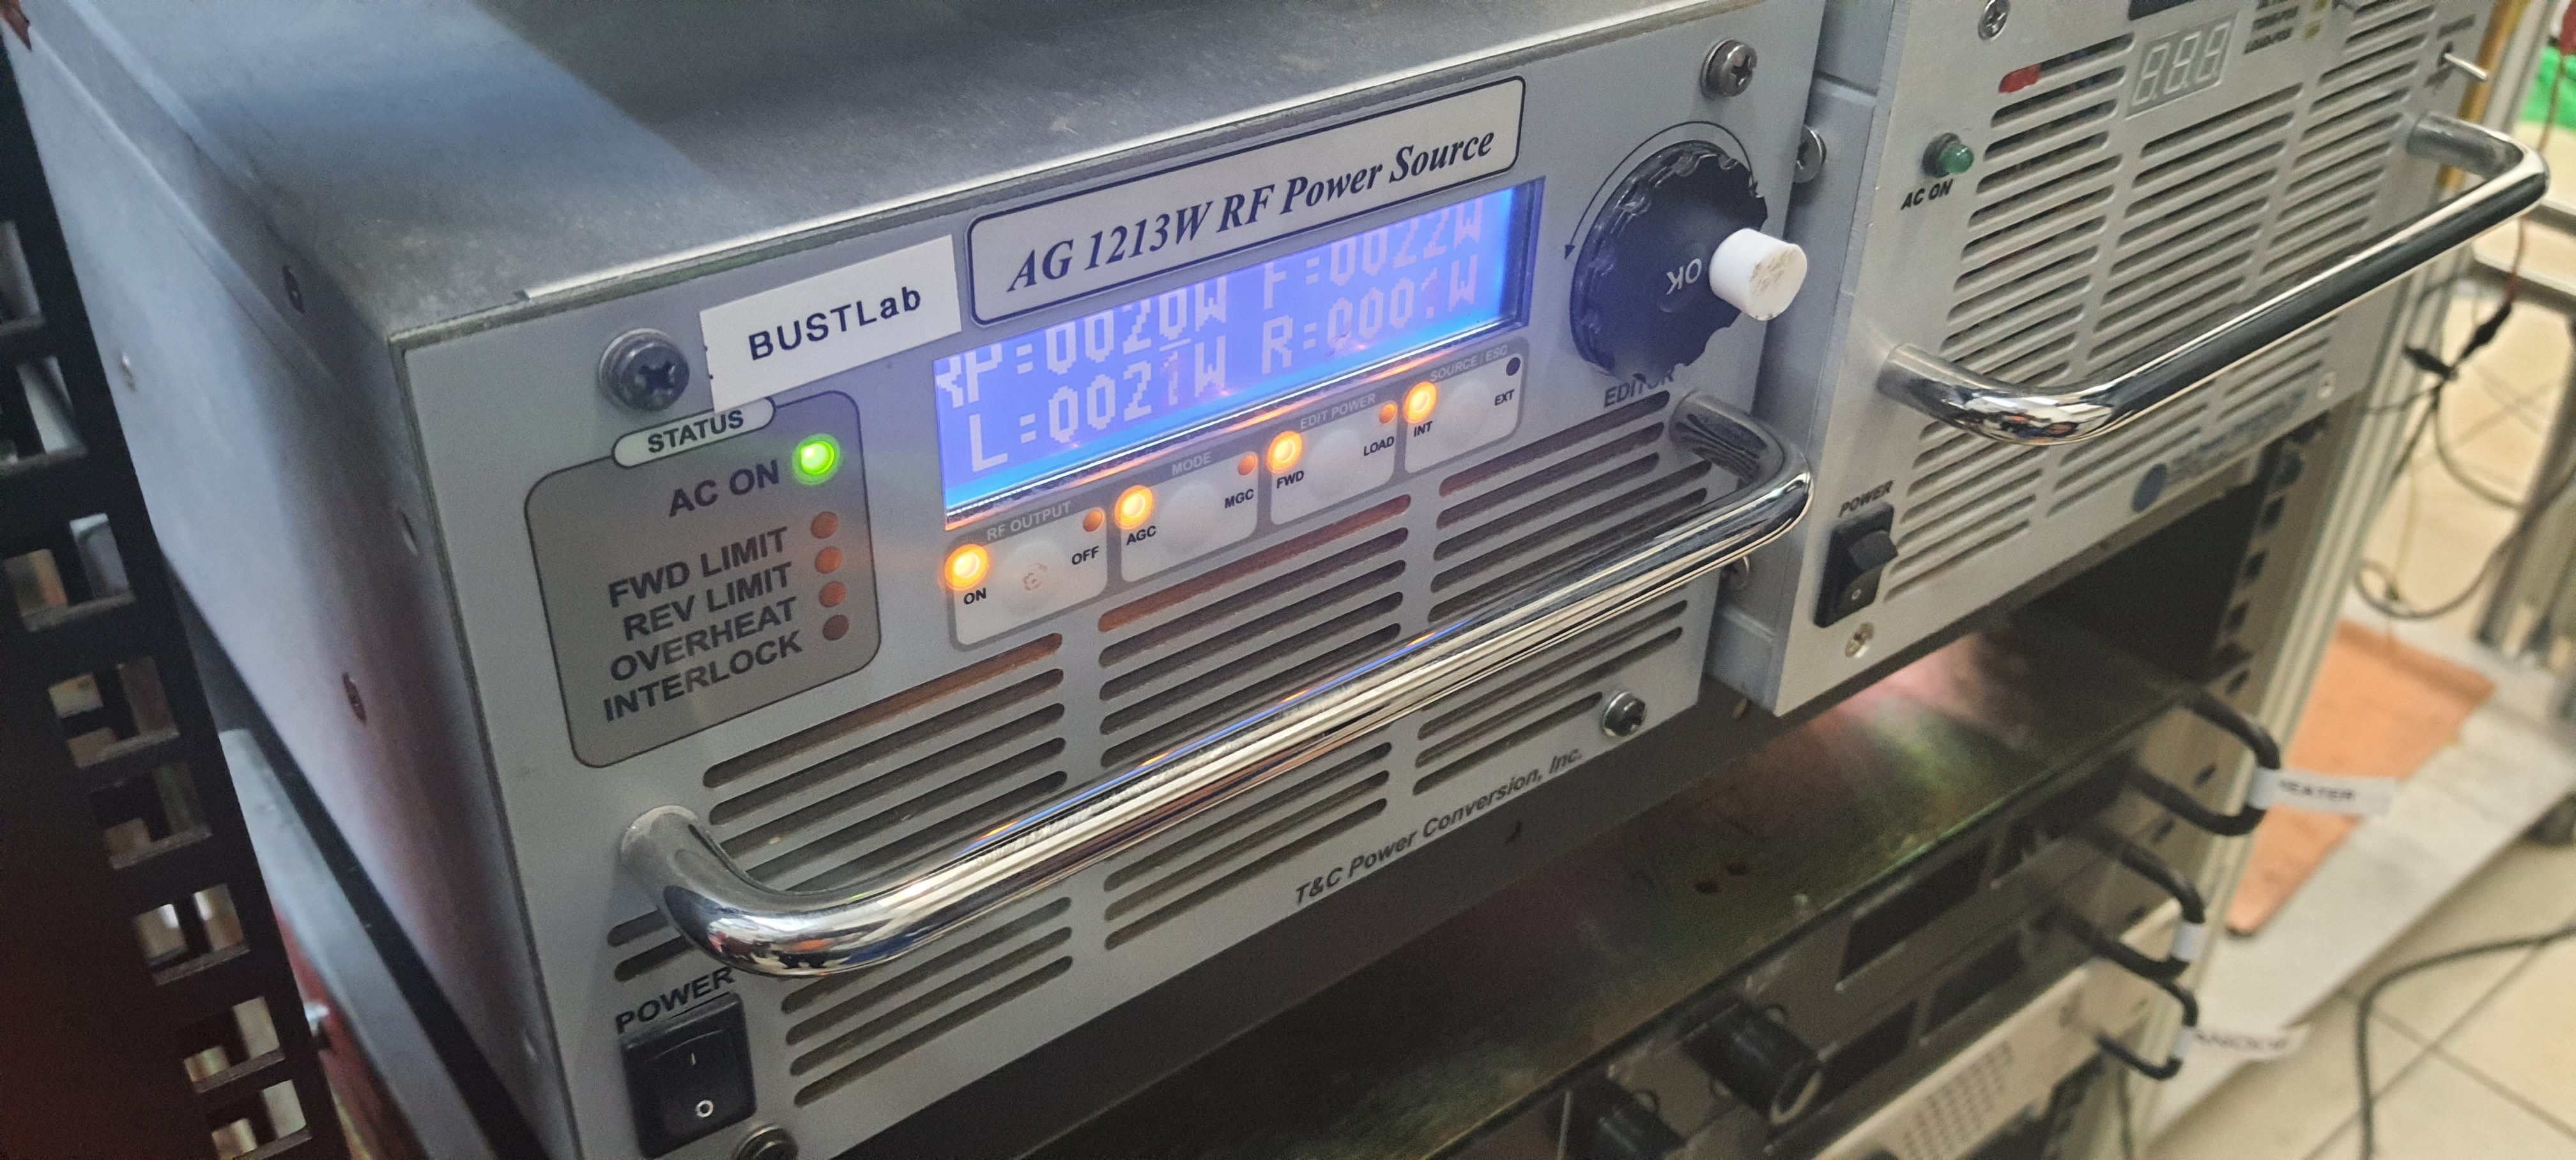
\includegraphics[height=6cm]{fig/rfpowersup.jpg}
    \caption{RF power source}
    \label{fig:rfpowersup}
\end{figure}

A LED screen displays set output power, forwarded power, load power and reflected power. Through load and reflected power impedence mismatch can be determined which will be discussed in the following subsection.

\subsection{Matching Network} \label{ch:Ch4_mn}
Since RF coil will used to broadcast a signal its impedance value carries a significance. Impedance is the opposition of alternating current(AC) flow which carries the RF signal\cite{slurzberg1950essentials}. It is represented with SI unit of ohm($\Omega$). If there is an impedence mismatch between the source and the antenna then signal transmission is significantly hindered. Usually commercial and industrial RF products are manufactured to have a default of 50$\Omega$ impedance. For example signal source used for this product, AG1213W, is defaulted to 50$\Omega$ of impedence.

Since RF coil used in this work is specifically designed for this thruster, its impedence is not compatible with that of RF power source's. In order to match the impedence value of the antenna, or load, to signal generator, or source, an electronic circuit is introduced to the system. This process is called network matching. For this work Palstar AT2K 2000W network tuner, shown in figure \ref{fig:tuner}, is used to match the network.

\begin{figure}[ht] 
    \centering
    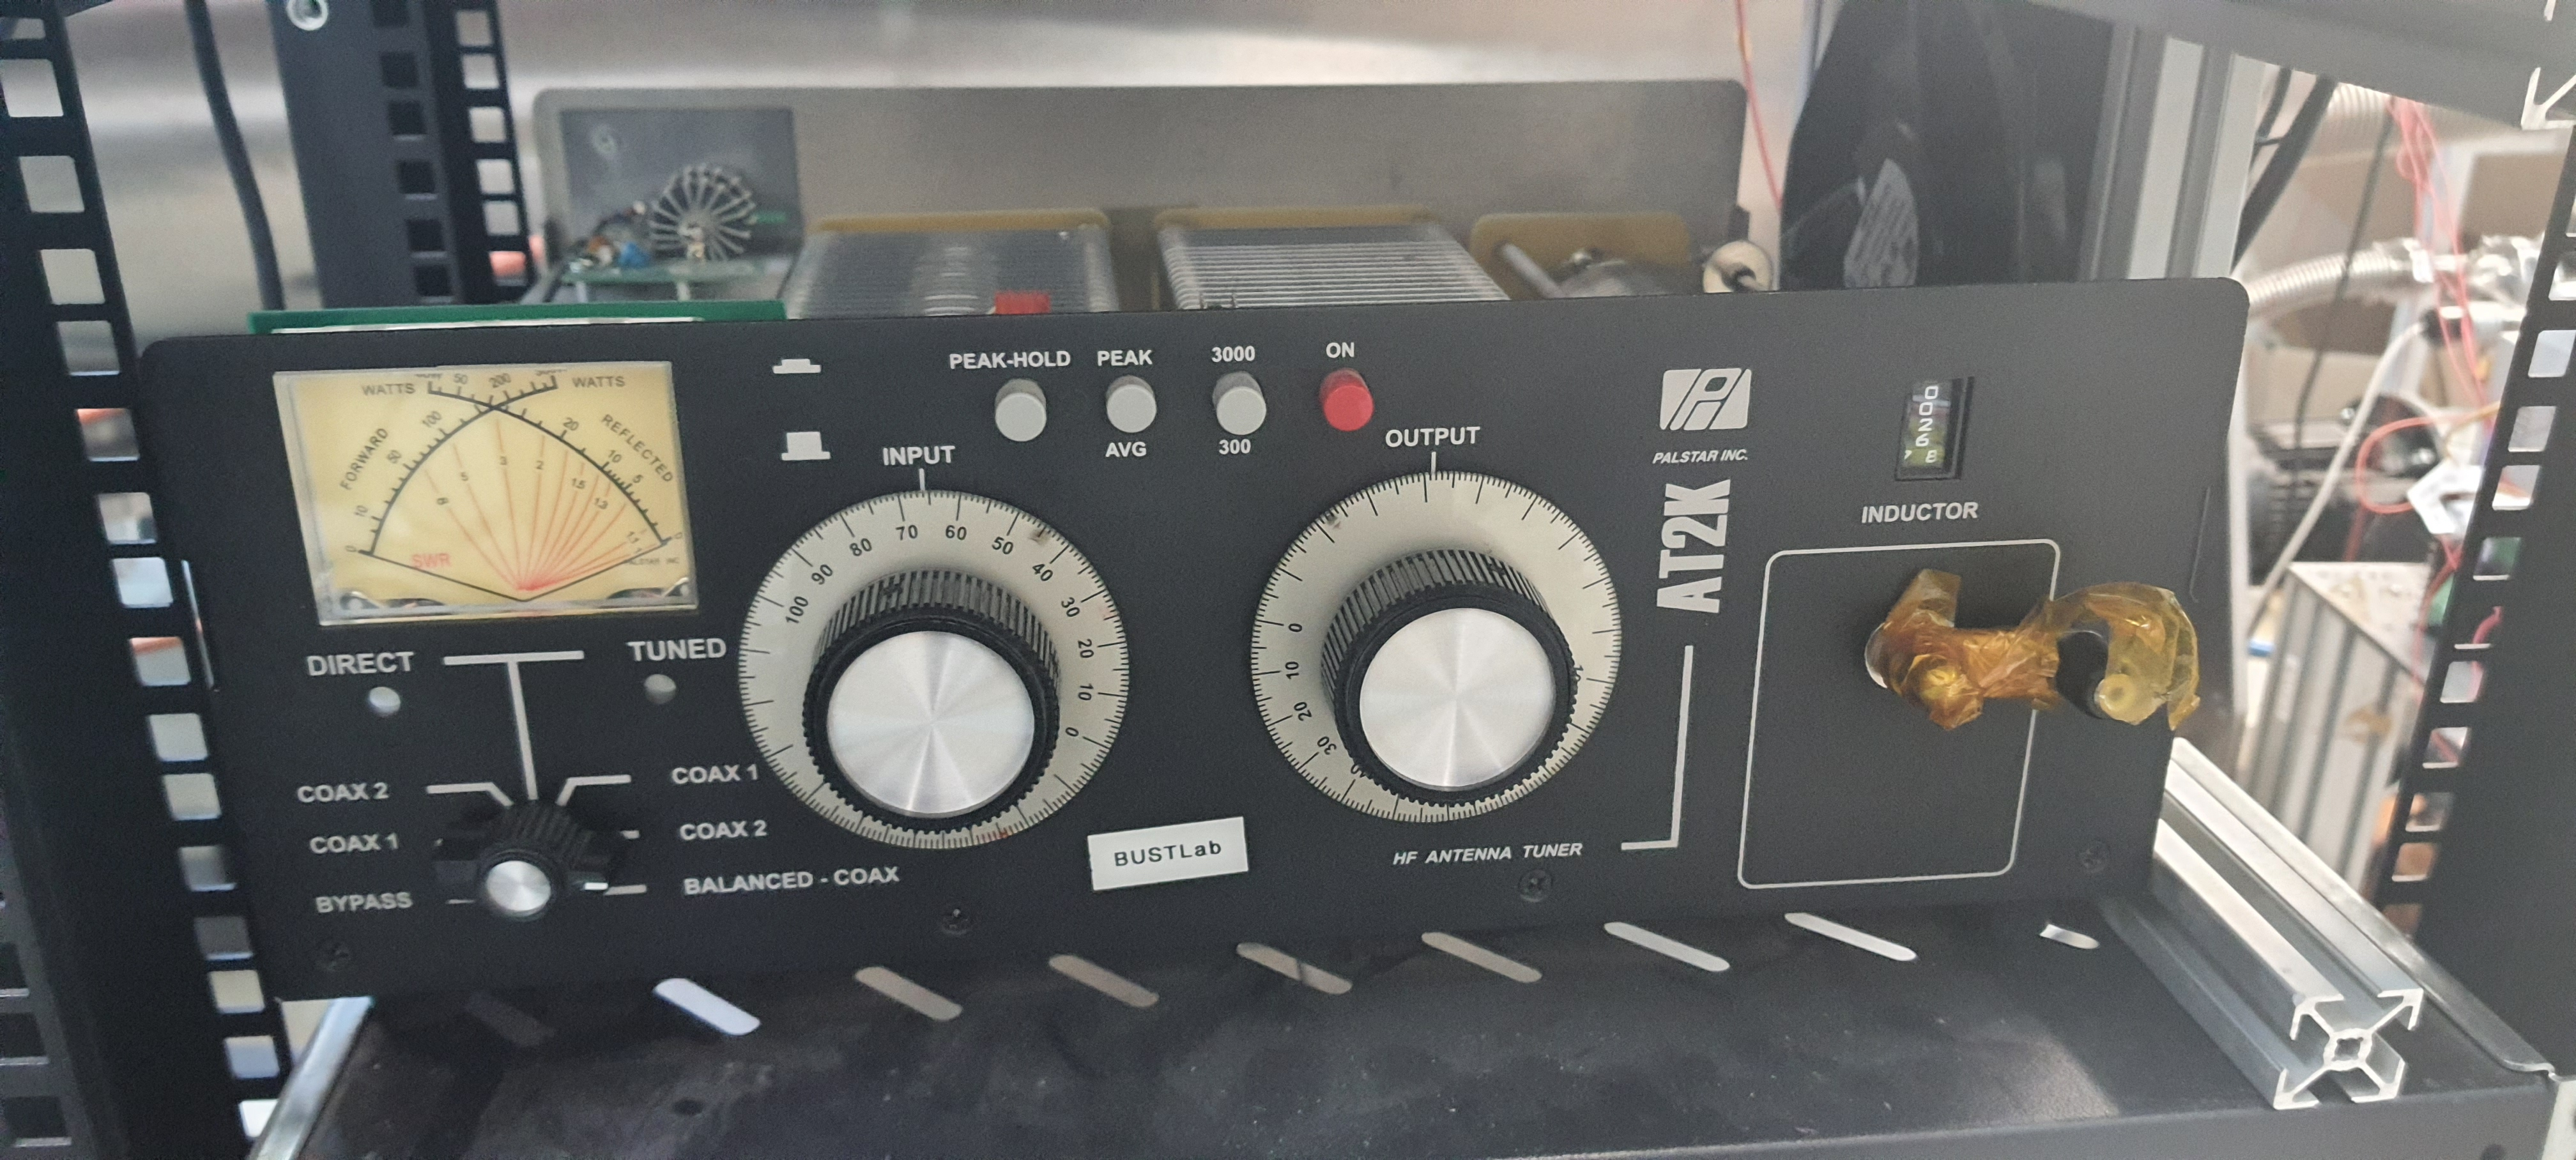
\includegraphics[height=6cm]{fig/tuner.jpg}
    \caption{Network tuner}
    \label{fig:tuner}
\end{figure}

This tuner consists of two variable capacitors and a variable inductor. Two capacitors are connected in series and the inducter is connected in parallel(shunt) to complete the circuit. On the front side of the tuner is an SWR (standing wave ratio) meter which shows reflected and forwarded power similar to the RF signal source. Based on this SWR meter transmitted signal power is determined. 

Types and working mechanisms of matching networks are explained in detail in appendix \ref{ch:appndxB_RF}.
% In this section, information will be given about how citations, quotings and footnotes should be.
\subsection{DC Power Supplies}
Two DC power supplies, one for each grid, are needed. There are three DC power supplied present within the laboratory. Two of them are Sorenson brand, models DCS60-18E and DCS600-1.7E which can output 60V-18A and 600V-1.7A respectively. Third power supply is Glassman brand and can provide 1500V-1.5A. They are shown in figure \ref{fig:dcpowersups}.

\begin{figure}[ht] 
    \centering
    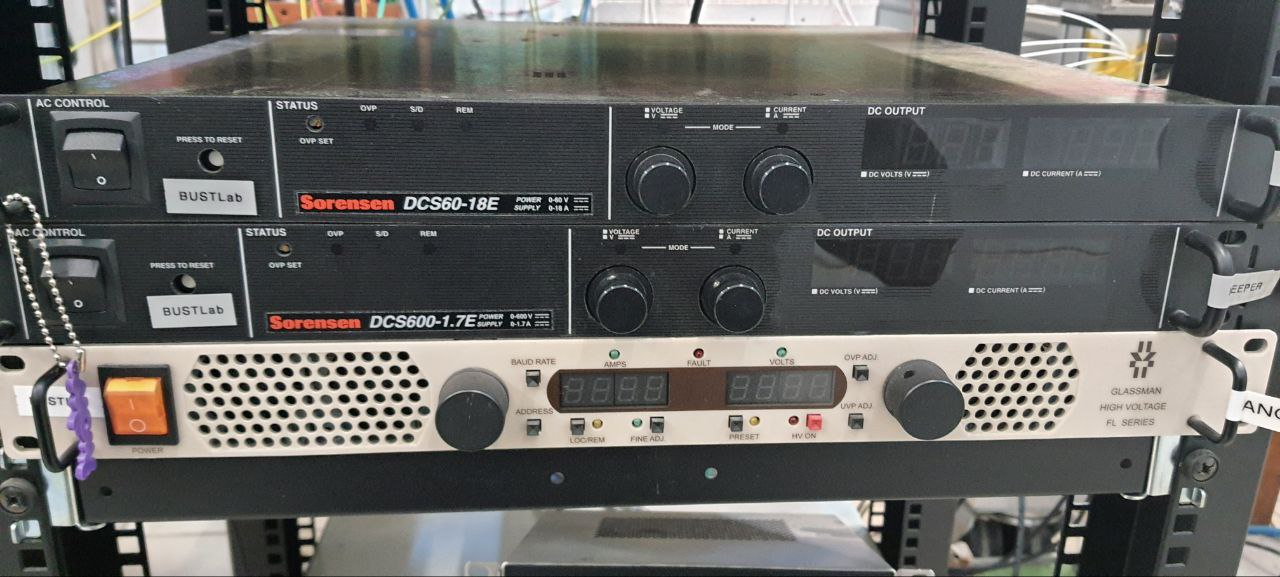
\includegraphics[height=6cm]{fig/dcpowersups.jpeg}
    \caption{DC Power supplies}
    \label{fig:dcpowersups}
\end{figure}

\subsection{Propellant Feed Line and Flow Controller}
Argon propellant is kept at pressurized tanks. Flow rate of propellant into the discharge chamber is important and is controlled by a MKS PR4000B type flow controller shown in figure \ref{fig:flowcont}. It displays the flow are in units of cubic centimeters per minute (SCCM). 

\begin{figure}[ht]
    \centering
    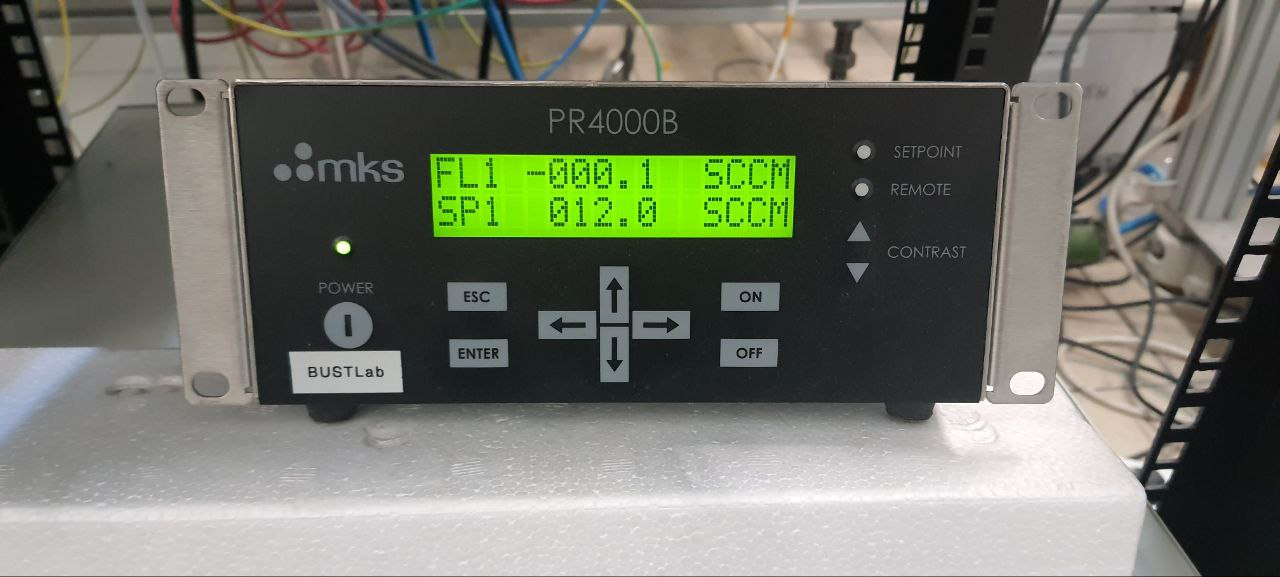
\includegraphics[height=7cm]{fig/flowcontroller.jpeg}
    \caption{Flow controller}
    \label{fig:flowcont}
\end{figure}

A feedthrough is used to drive the propellant lines through vacuum chamber as shown in figure \ref{fig:propfeedthr}. There are two feed lines are present. Feedline 1 can support flow rates up to 25 SCCMs whereas feedline 2 can support flowrates up to 1000 SCCMs.

\begin{figure}[ht]
    \centering
    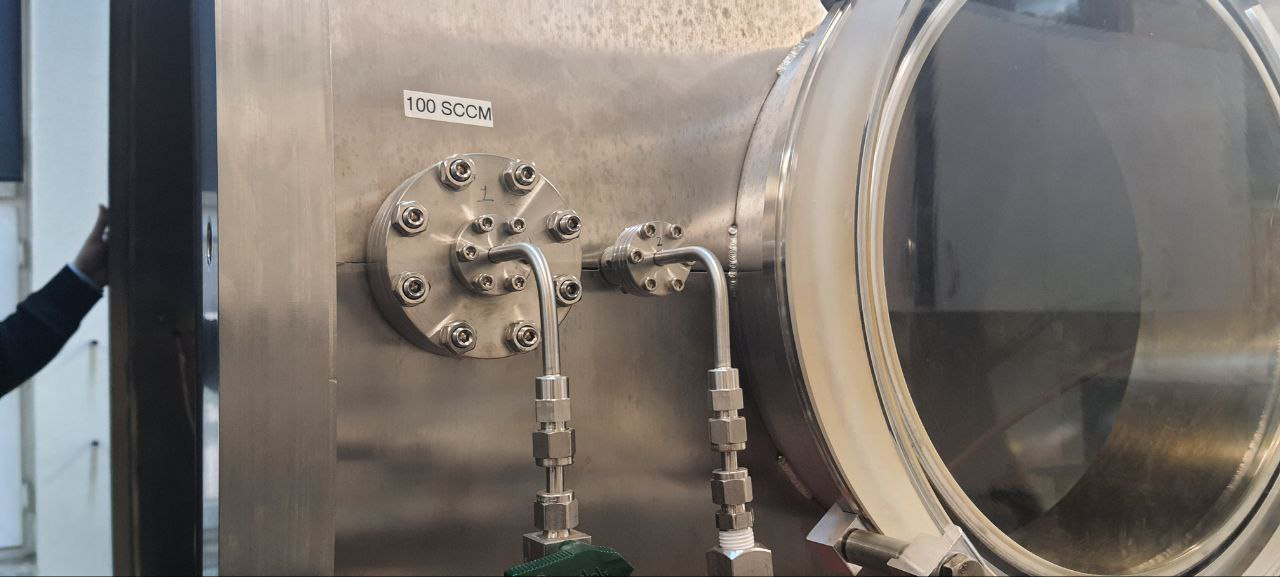
\includegraphics[height=5cm]{fig/propfeedthr.jpeg}
    \caption{Propellant feedthrough}
    \label{fig:propfeedthr}
\end{figure}



% \subsection{Methodology}
% \section{Citing (indication of references in main text body)}
% \section{Input Parameters}

% \subsection{Citing according to surname of author}

% References are cited with the surname of author and year. In the references section, the references are listed alphabetically according to the surname of the author.

% Citing of a reference at the beginning of or within a sentence must be as Boran (2003), whereas a citation at the end of a sentence must be as (Boran, 2003). The full-stop is placed directly after the citation.
 
% A reference with two authors must be cited as Yılmaz and Johnson (2004) at the beginning of or within a sentence, or as (Yılmaz and Johnson, 2004) at the end of a sentence. 

% A reference with more than two authors must be cited as Yılmaz et al. (2004) at the beginning of or within a sentence, or as (Yılmaz et al, 2004) at the end of a sentence. 

% Different publications of an author published in the same year must be cited as Feray (2005a), Feray (2005b). 

% While citing a part of a publication; the number of the page the cited material (chapter, table, figure, or equation) is on must be indicated. While citing, the expression “page” must be abbreviated, but “chapter” must not. For example; (Centers for Disease Control and Prevention, 2005, p. 10), (Shimamura, 1989, Chapter 3). 

% Citing multiple publications in one pair of brackets; (Berndt, 2002; Harlow, 1983). 

% Citing personal communication in main text body; (V.–G. Nguyen, personal communication, September 28, 1998), (J. Smith, personal communication, August 15, 2009).

% In the references section, reference tags must be listed according to the surname of author. 

% For citing of secondary references (In case the reference cites another reference), the secondary reference must be cited in brackets.  In the references section, the reference tag is organized according to the secondary reference, the original reference must not be used as a tag. For example; In his e-mails, Smith argued that asynchronous line dancing would be the next Internet meme (as cited in Jones, 2010).

% \subsection{Citing according to order of appearance}

% References are cited by numbering and indicating the number in square brackets ([]) in the main text body. The first reference cited in a thesis is numbered [1] and the following references are numbered according to the order of appearance. 

% In the main text body, references must be cited as specified below:
% \vspace*{-12pt}
% \begin{tabbing}
% \hspace*{1.5cm}\= \kill
% [1]      \> Reference no. 1\\

% [1--3]   \> References from no.1 to 3 (thus, references 1,2 and 3)\\

% [1,3]    \> References no. 1 and 3\\

% [1,3,8]  \> References no.1, 3 and 8\\

% [1,3--8] \> References no.1, and from no.3 to 8 (thus, references 1, 3, 4, 5, 6, 7 and 8)
% \end{tabbing}
% \vspace*{-12pt}
% Different volumes of a reference must be cited and numbered individually.
\newpage
\section{Experimental Procedure}
% \subsection{Thruster Placement}
% \subsection{Faraday Cup Placement}
A number of firing tests were conducted using systems described above. Thruster is placed inside the vacuum chamber. It was placed on a makeshift table in order to make it easier to observe through the windows of the vacuum chamber. Placement of the thruster is shown in figure \ref{fig:invacuum_assm}.

\begin{figure}[h]
    \centering
    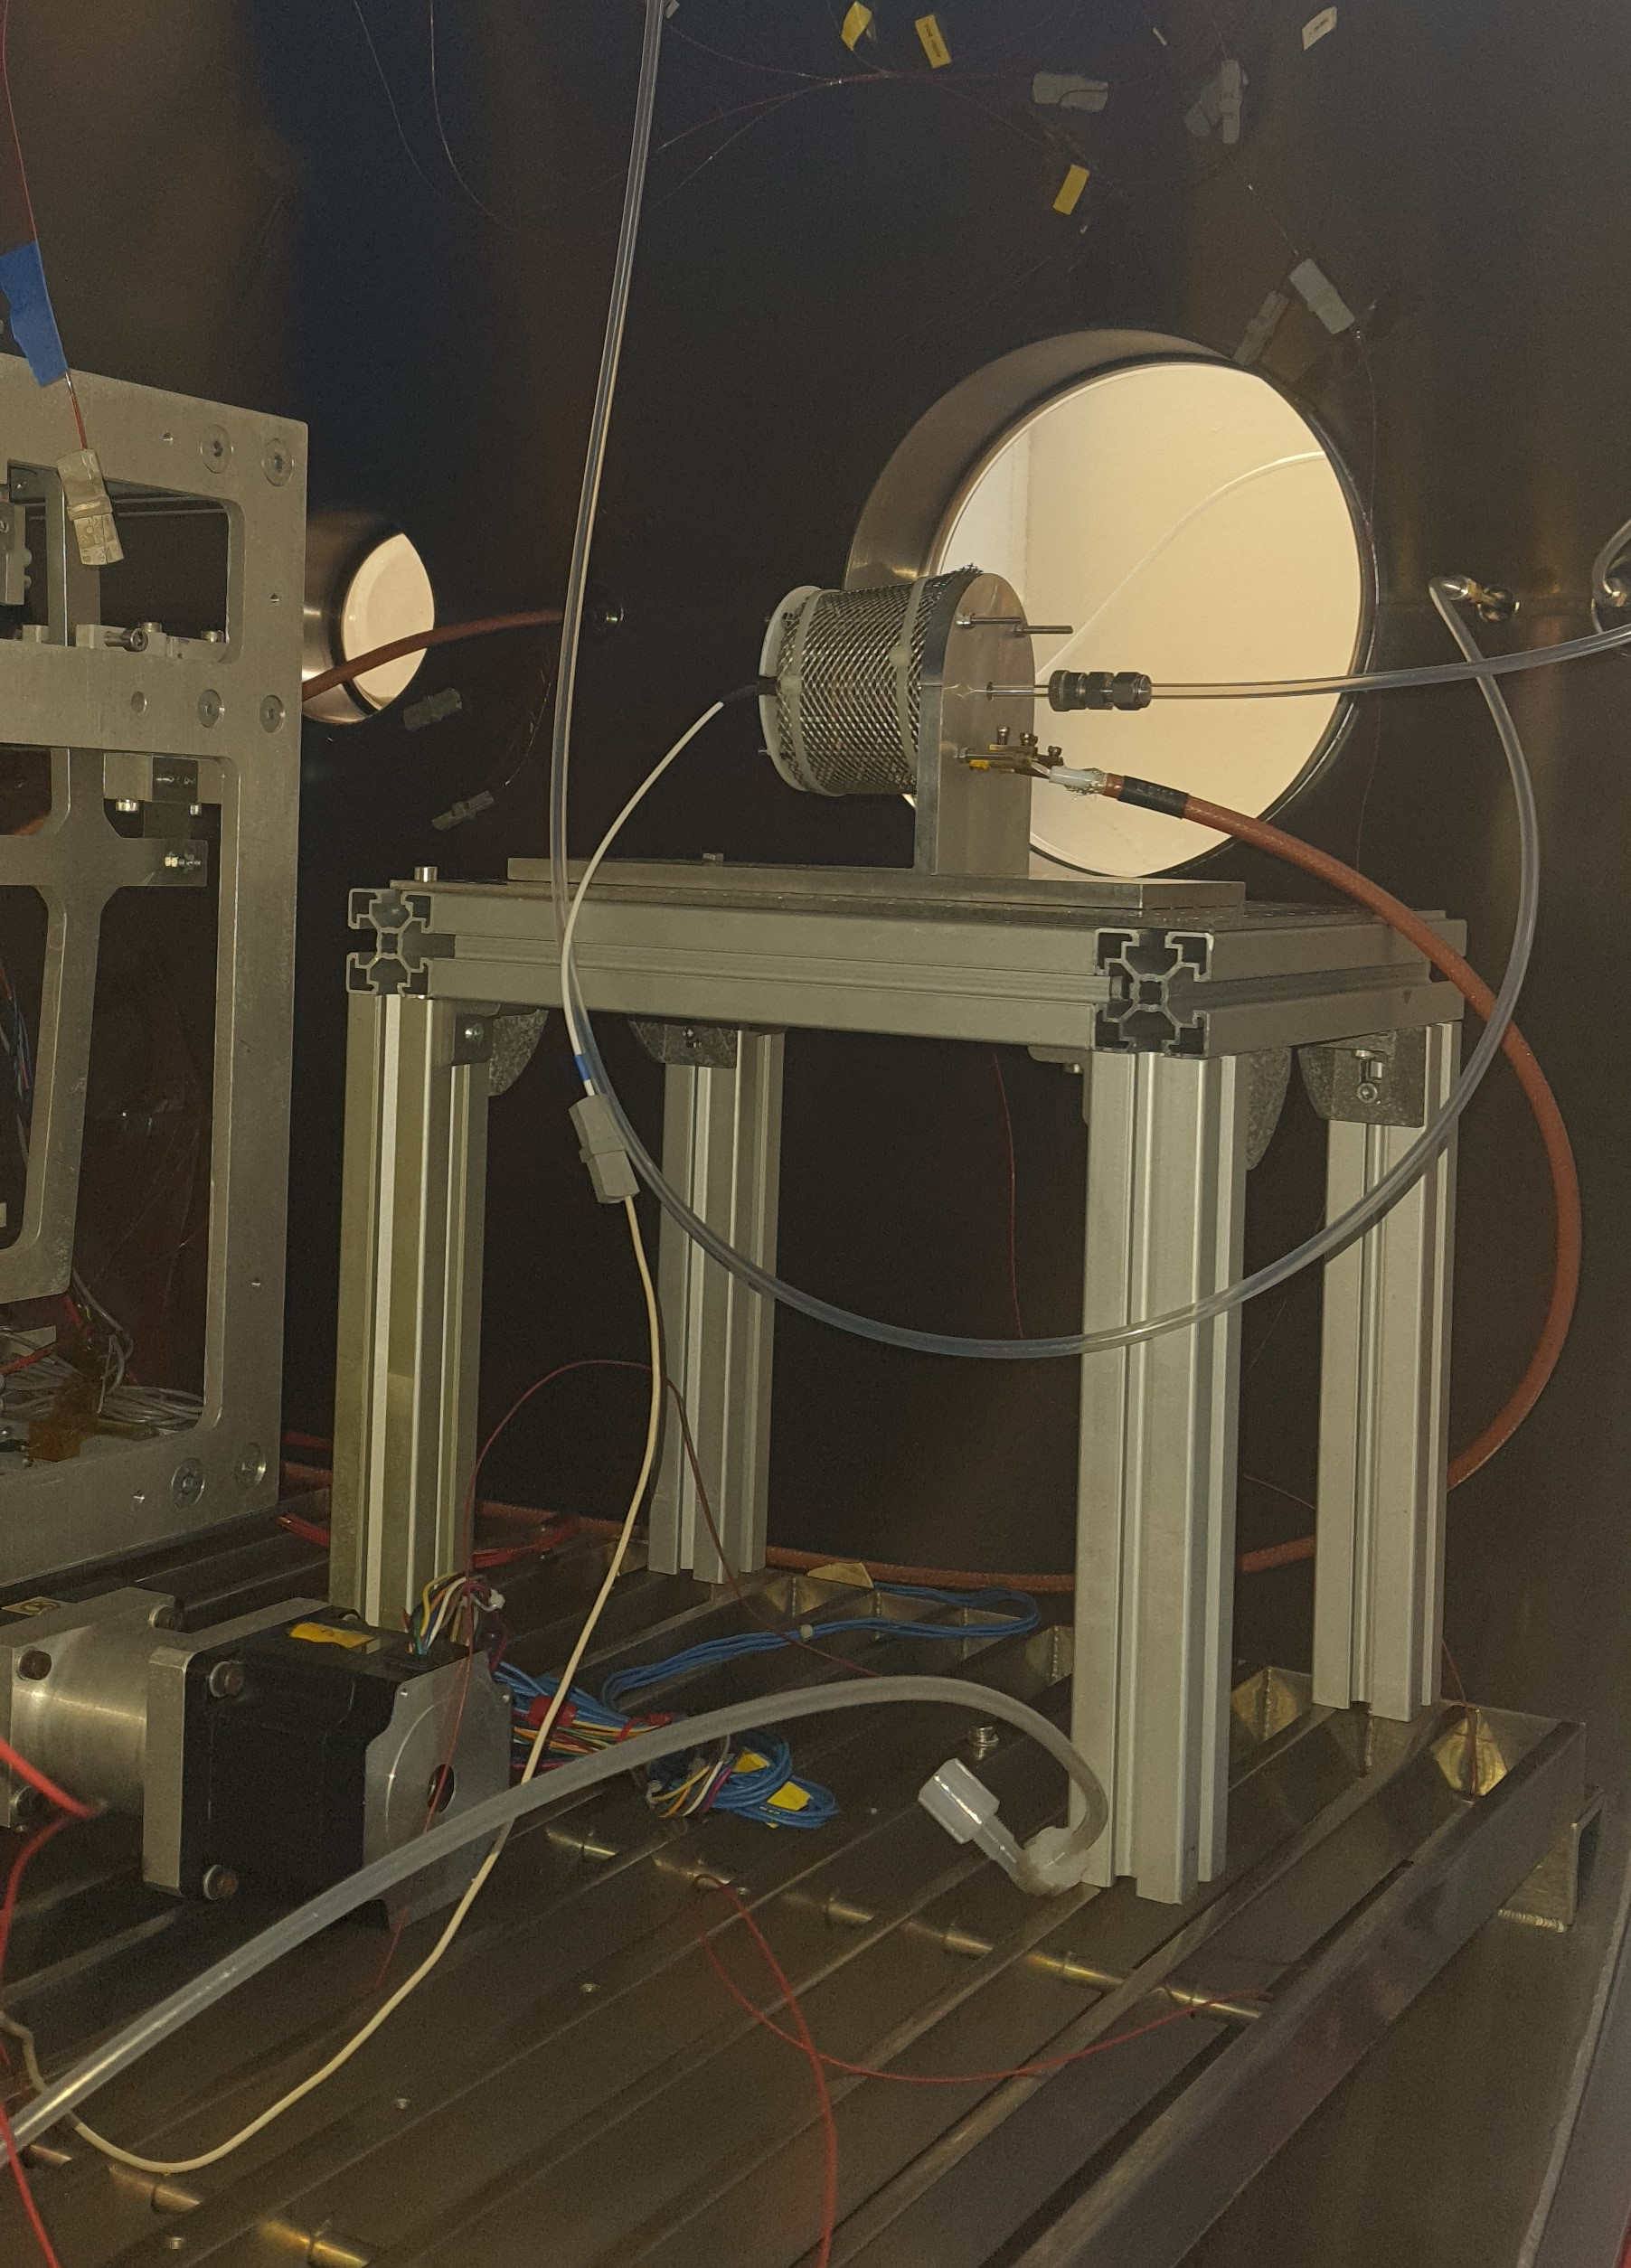
\includegraphics[scale=0.15]{fig/invacuum_assembly.jpg}
    \caption{Thruster within the vacuum chamber}
    \label{fig:invacuum_assm}
\end{figure}

RF signal is carried to the thruster via RG 393 cable. RF and DC connection cables were run through feedthroughs of the vacuum chamber and connected to the thruster via clamps. Propellant feed line is connected to the narrow end of the discharge chamber. All connections are shown in \ref{fig:invacuum_accel}, \ref{fig:invacuum_screen} and \ref{fig:invacuum_rf}. 
\newpage
\begin{figure}[h]
    \centering
    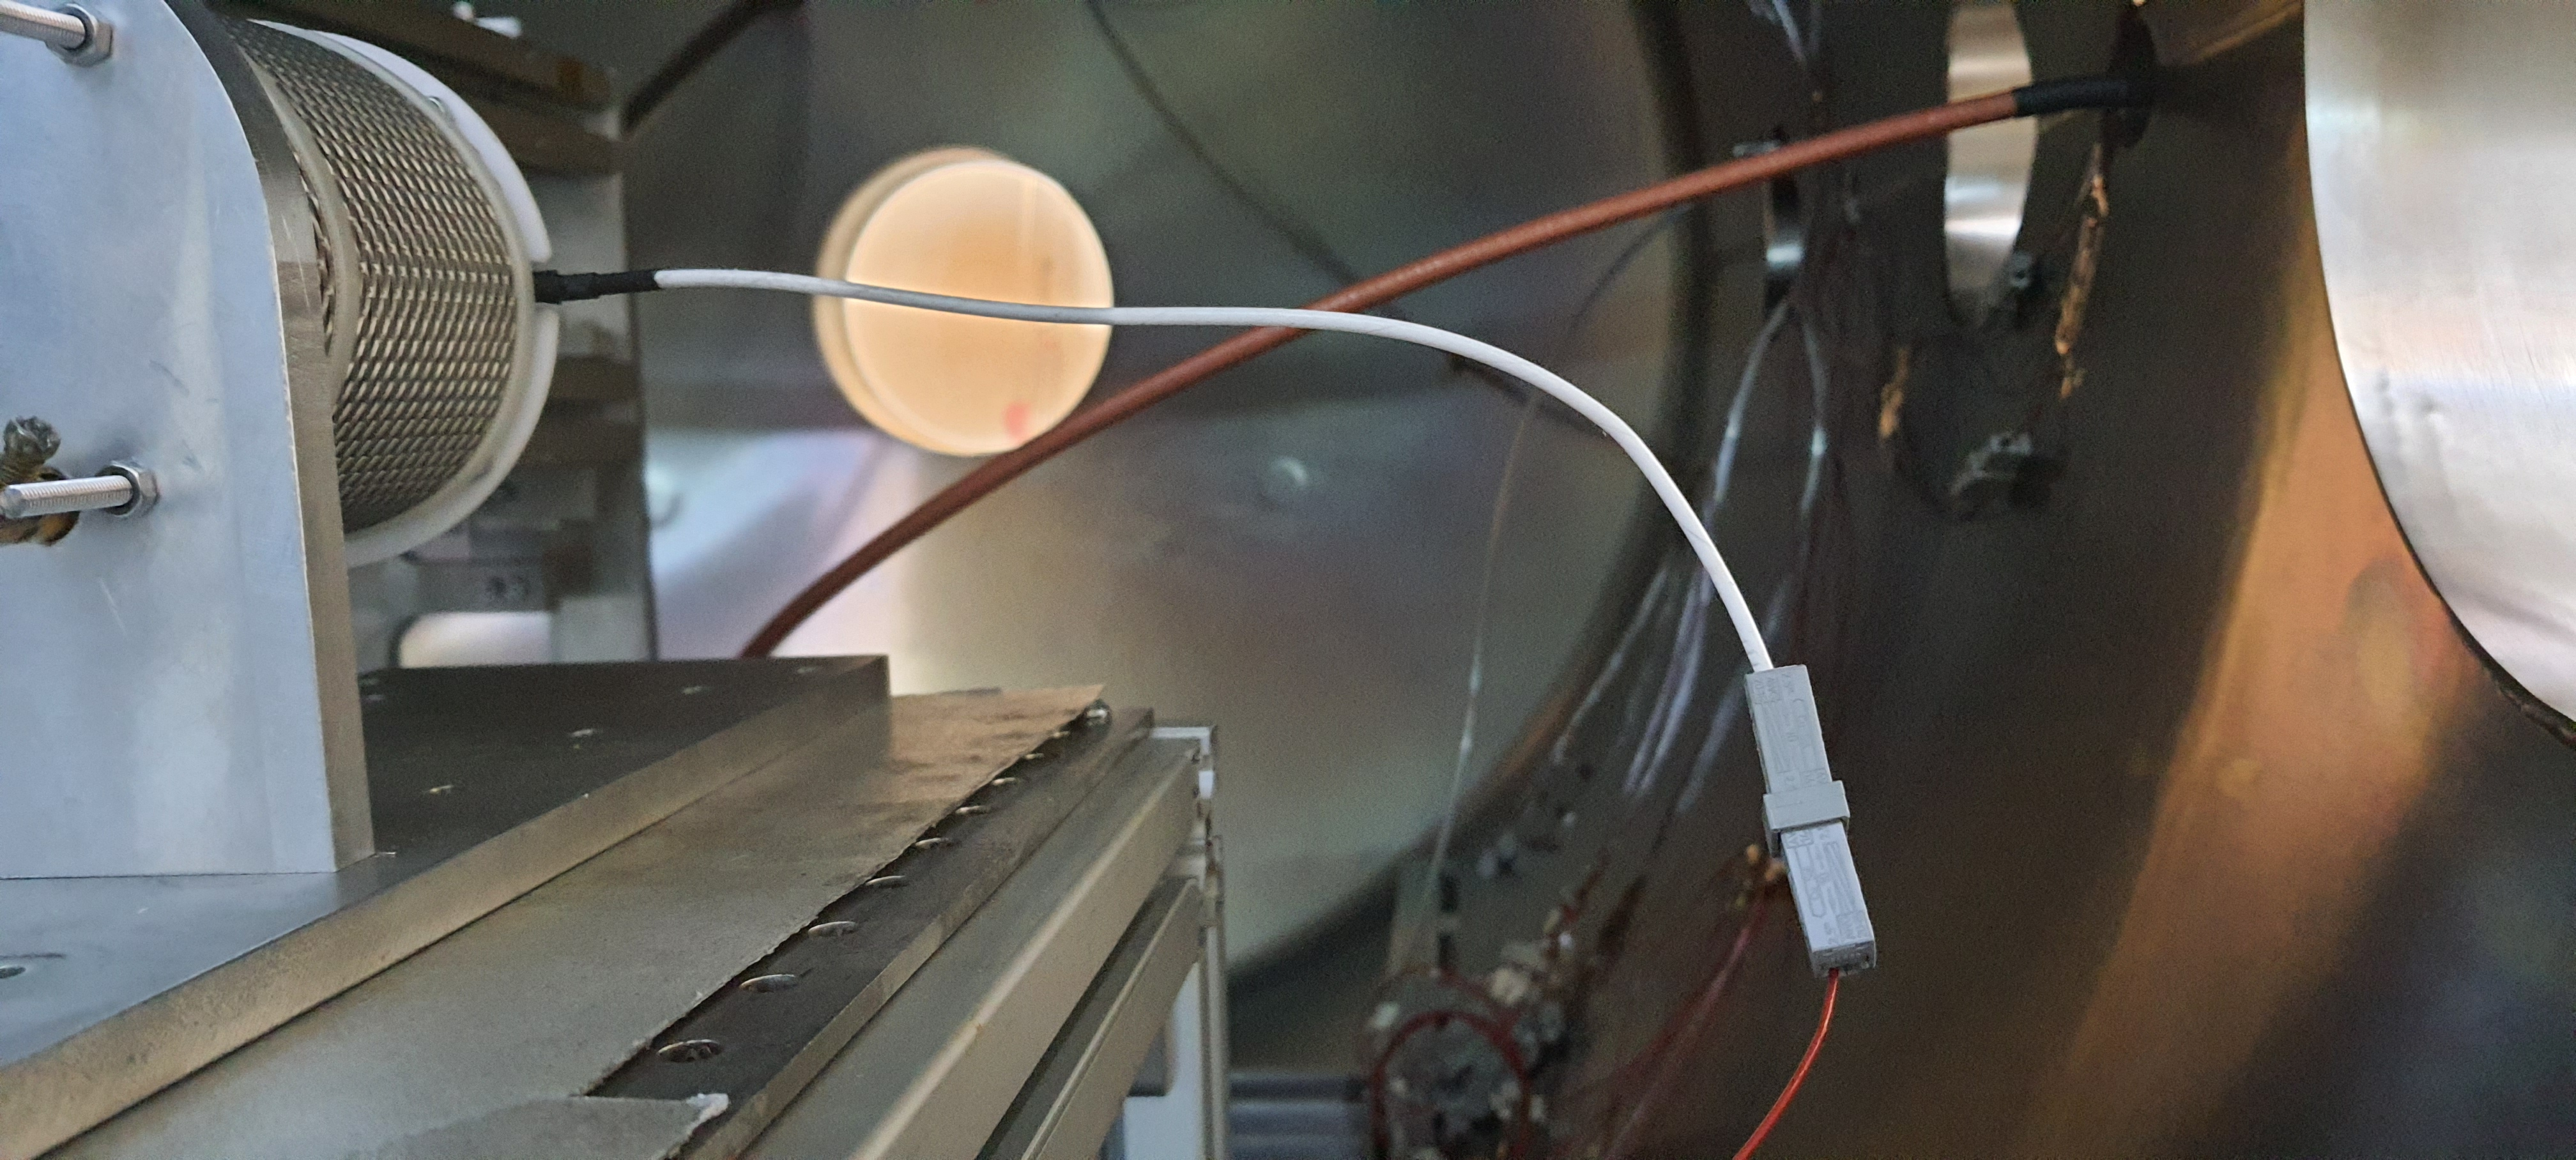
\includegraphics[scale=0.12]{fig/invacuum_accel.jpg}
    \caption{Connections of acceleration grid}
    \label{fig:invacuum_accel}
\end{figure}

\begin{figure}[h]
    \centering
    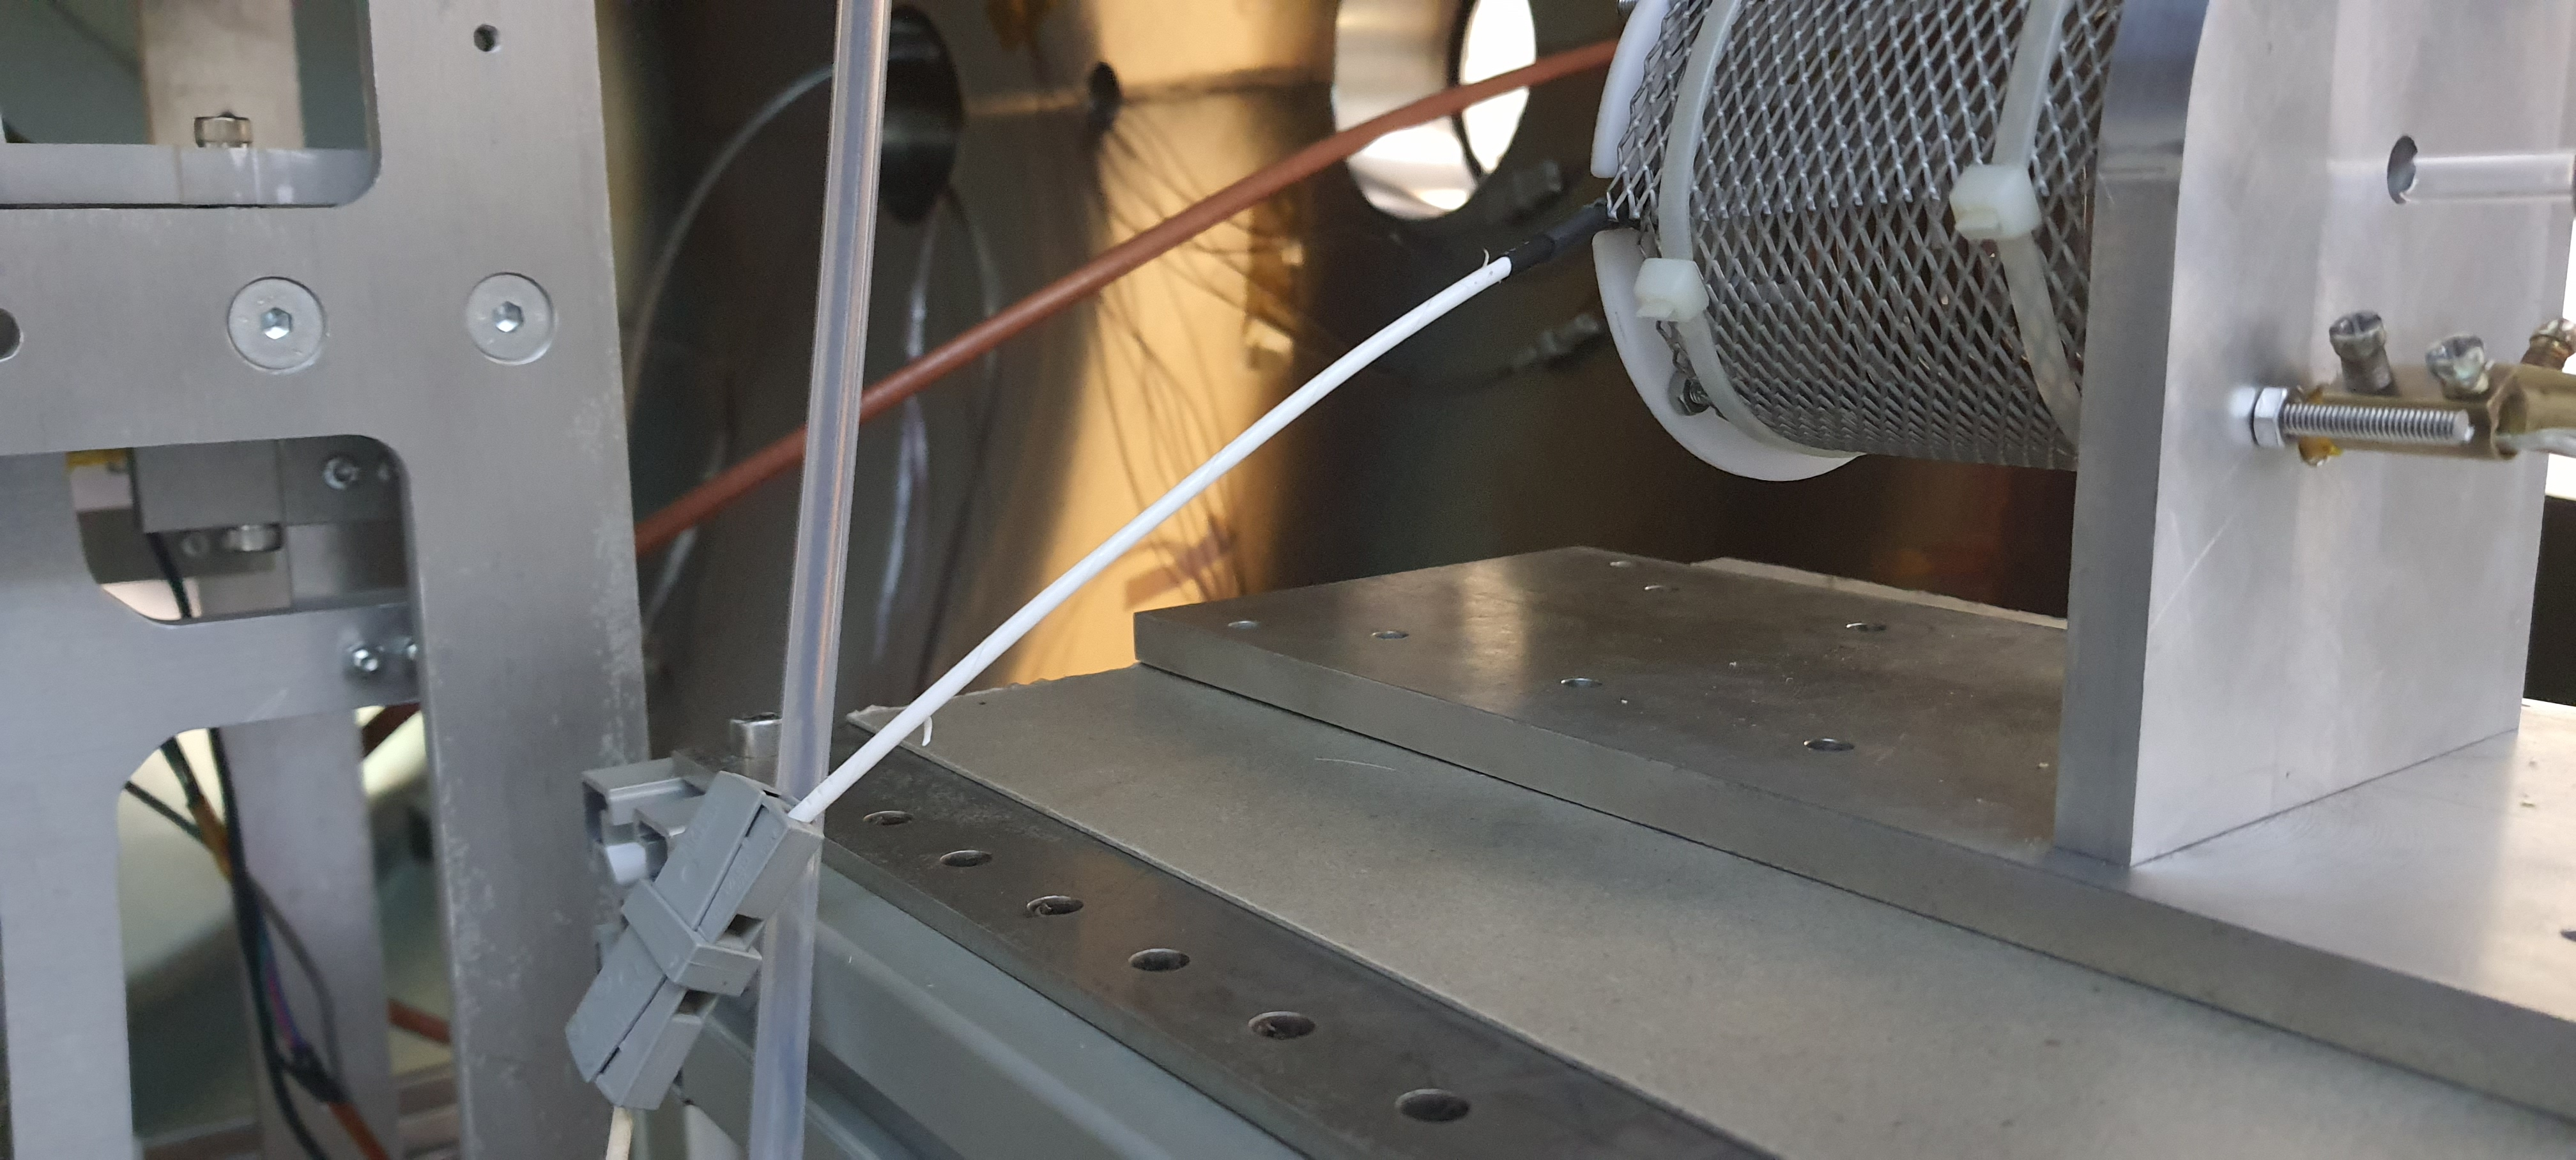
\includegraphics[scale=0.12]{fig/invacuum_screen.jpg}
    \caption{Connections of screen grid}
    \label{fig:invacuum_screen}
\end{figure}
\newpage
\begin{figure}[h]
    \centering
    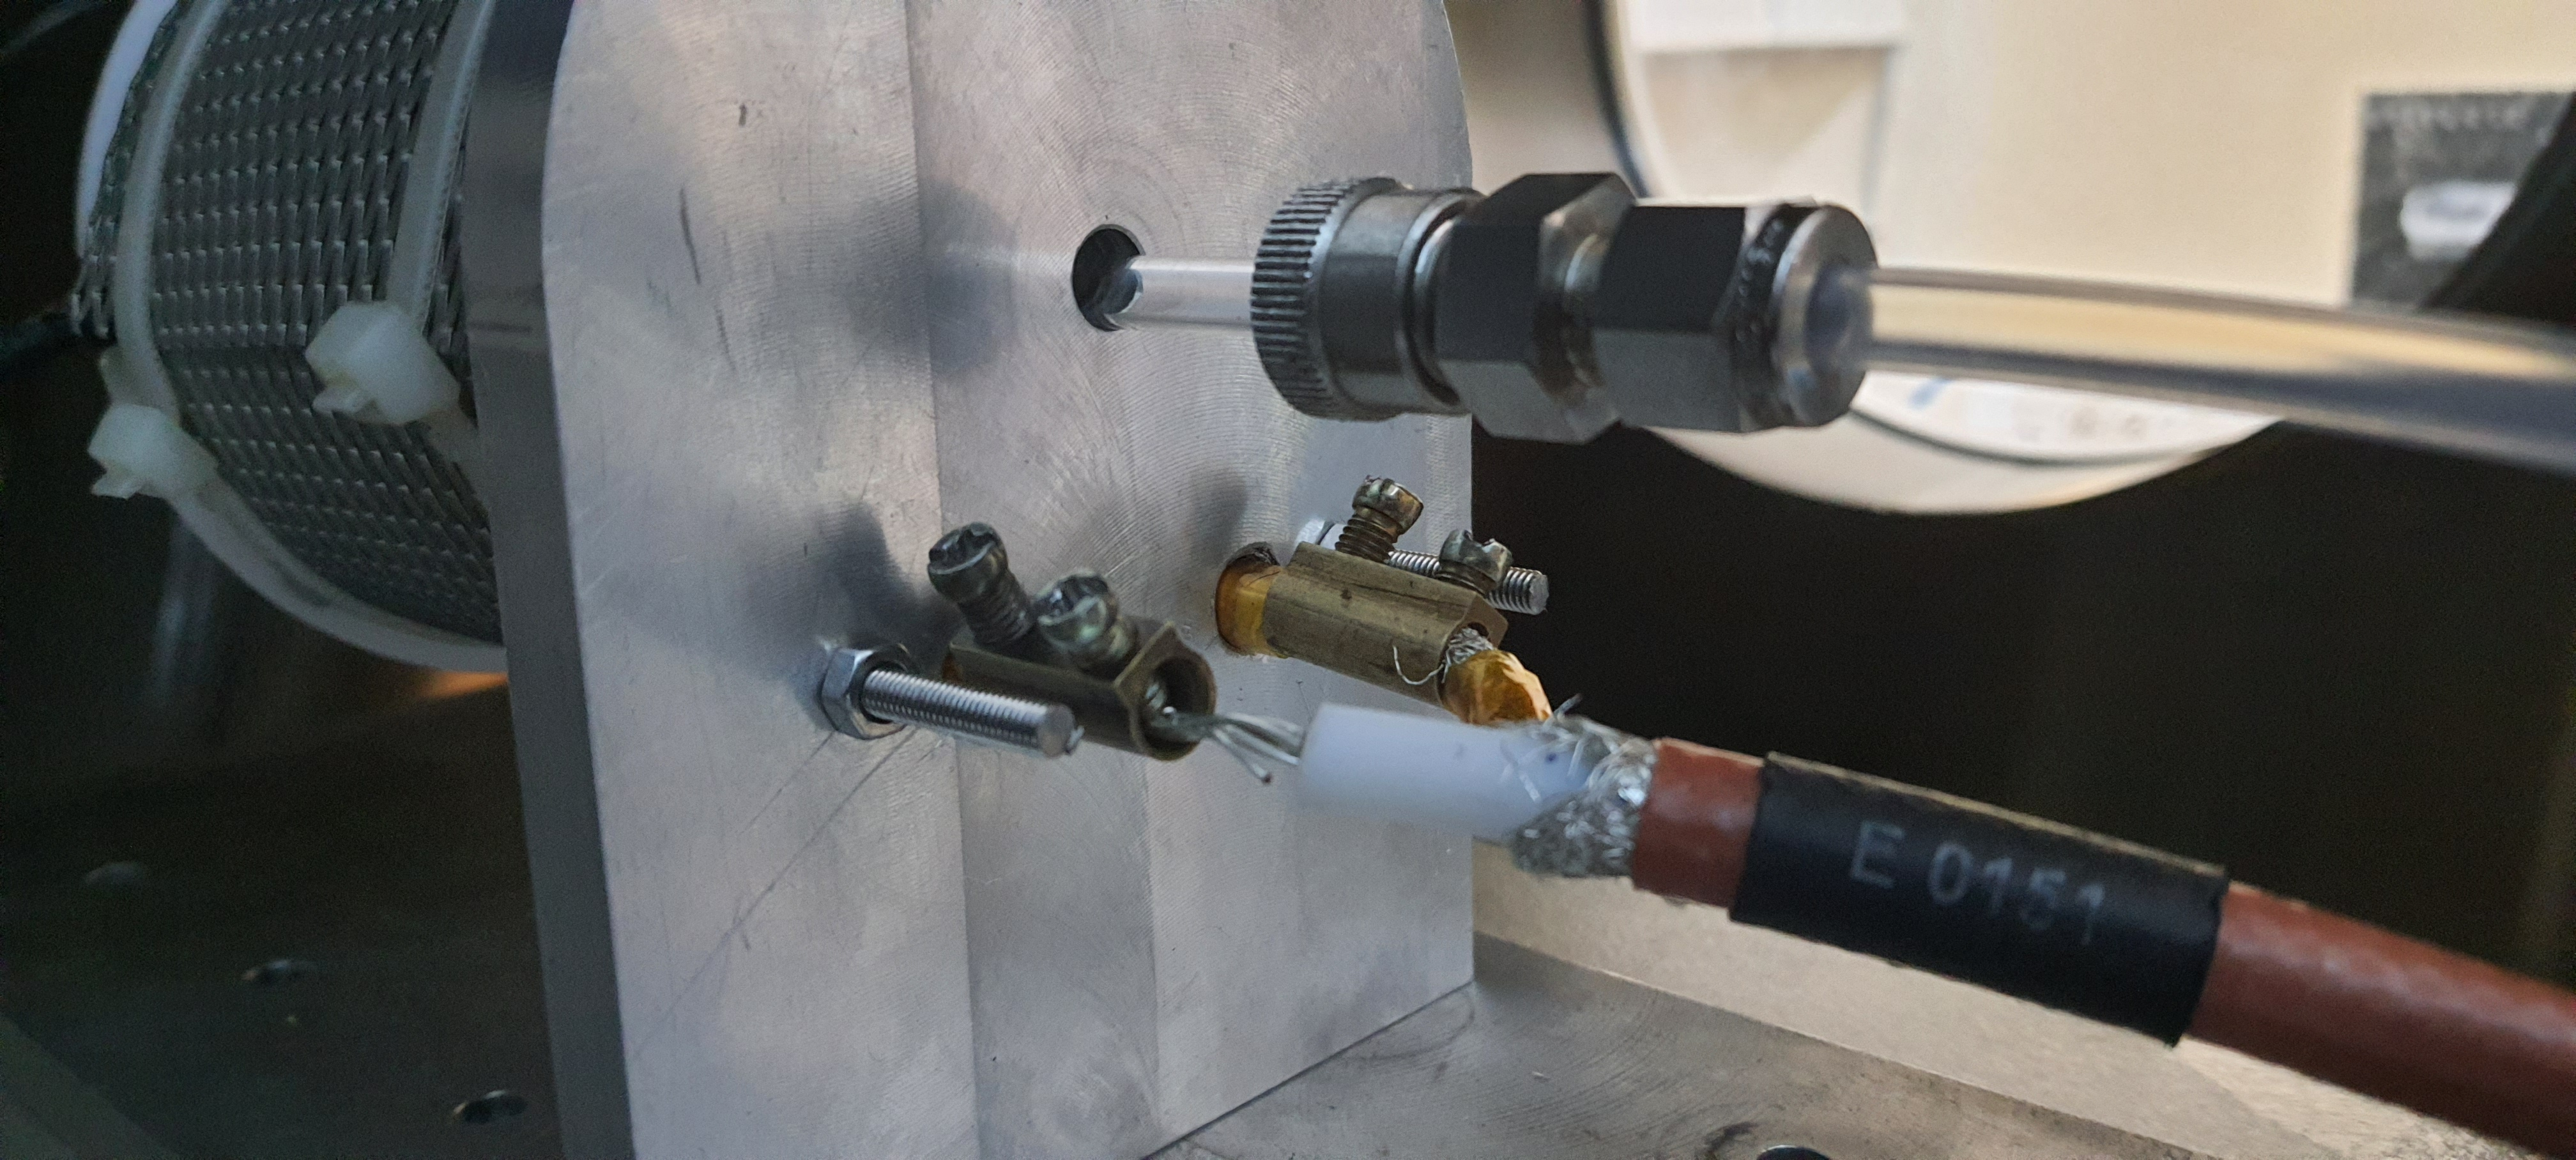
\includegraphics[scale=0.1]{fig/invacuum_rf.jpg}
    \caption{Connections of RF coil and propellant feedline}
    \label{fig:invacuum_rf}
\end{figure}

At this point impedance value of the RF coil is measured again.  It was discovered that the ground of the RF feedthrough is shorted to the entire vacuum chamber which created a different impedance value reading compared to the original measurements of the RF coil previously shown in figure \ref{fig:smithchart_meas}. Results of the new measurement is shown in figure \ref{fig:smithchar_meas_comb}.

\begin{figure}[h]
    \centering
    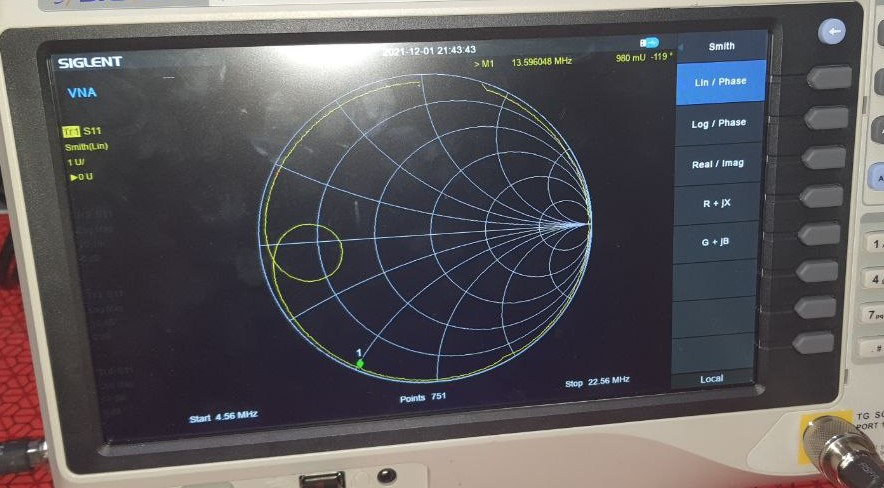
\includegraphics[scale=0.5]{fig/antenna_meas_combined.jpeg}
    \caption{Impedance value of coil combined with vacuum chamber}
    \label{fig:smithchar_meas_comb}
\end{figure}

Antenna tuner is included within the circuit to match the impedance values. Total circuit schematic is shown in figure \ref{fig:schematic}.

\begin{figure}[ht]
    \centering
    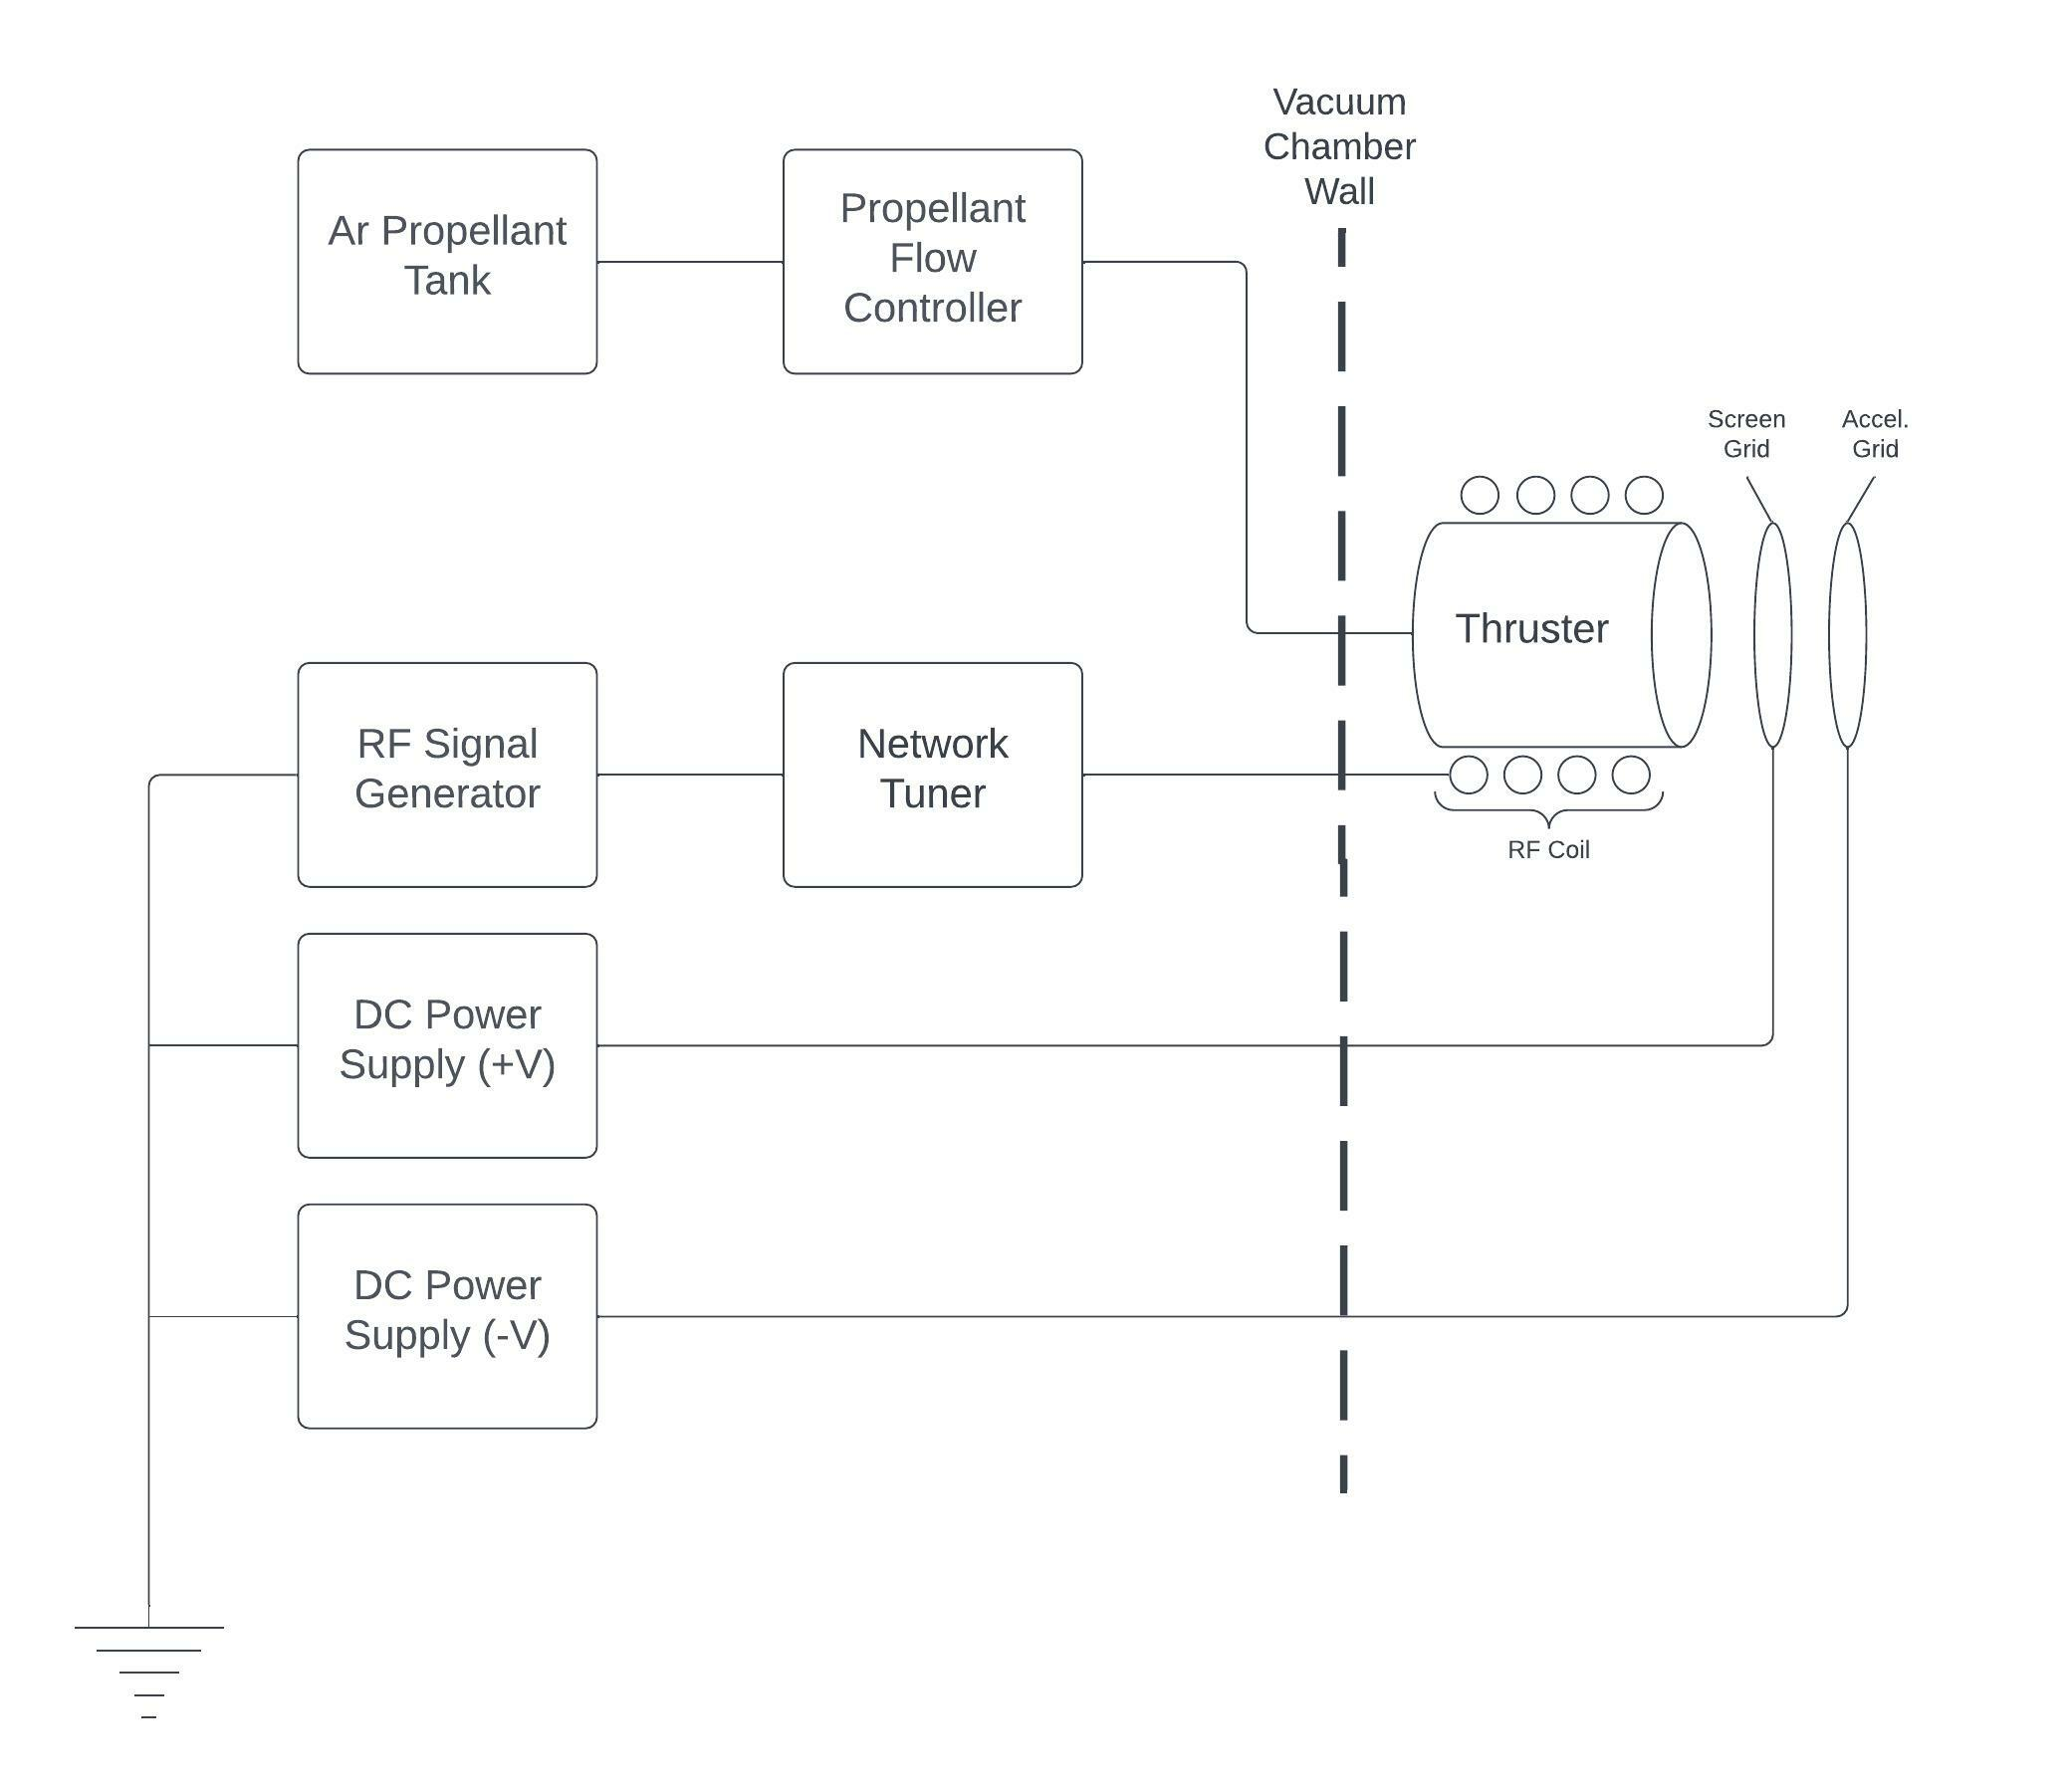
\includegraphics{fig/thrusterschematic.jpeg}
    \caption{Experimental setup schematic}
    \label{fig:schematic}
\end{figure}

After setting up the thruster a series of ignition tests were performed. Effect of different ion extractor grid, propellant flow rate, RF and DC power levels were examined throughout the tests. Initial tests failed due to number of reasons. Tests were conducted until a steady stream of ions were observed leaving the thruster. 

\newpage
\subsection{Firing Test No. 1}
During the first test pressure inside the vacuum chamber has been reduced down to $1.8x10^{-5}$ torrs. For this test ion extractor grids were made out of SS304 grade steel and they were manufactured using oxygen laser cutting process. Center to center distance of grid apertures were 3.2 mm and there were a total of 91 apertures. Signal between the RF source and antenna have been tuned to provide 1.02 SWR. Plasma inside the discharge chamber have been succesfully ignited with 5W of RF power and 13 SCCM propellant flow rate as shown in figure \ref{fig:1st_ccp}. Ignited plasma is observed to be capacitively coupled plasma (CCP) judging by the low power input and faint glow of plasma. 

\begin{figure}[ht]
    \centering
    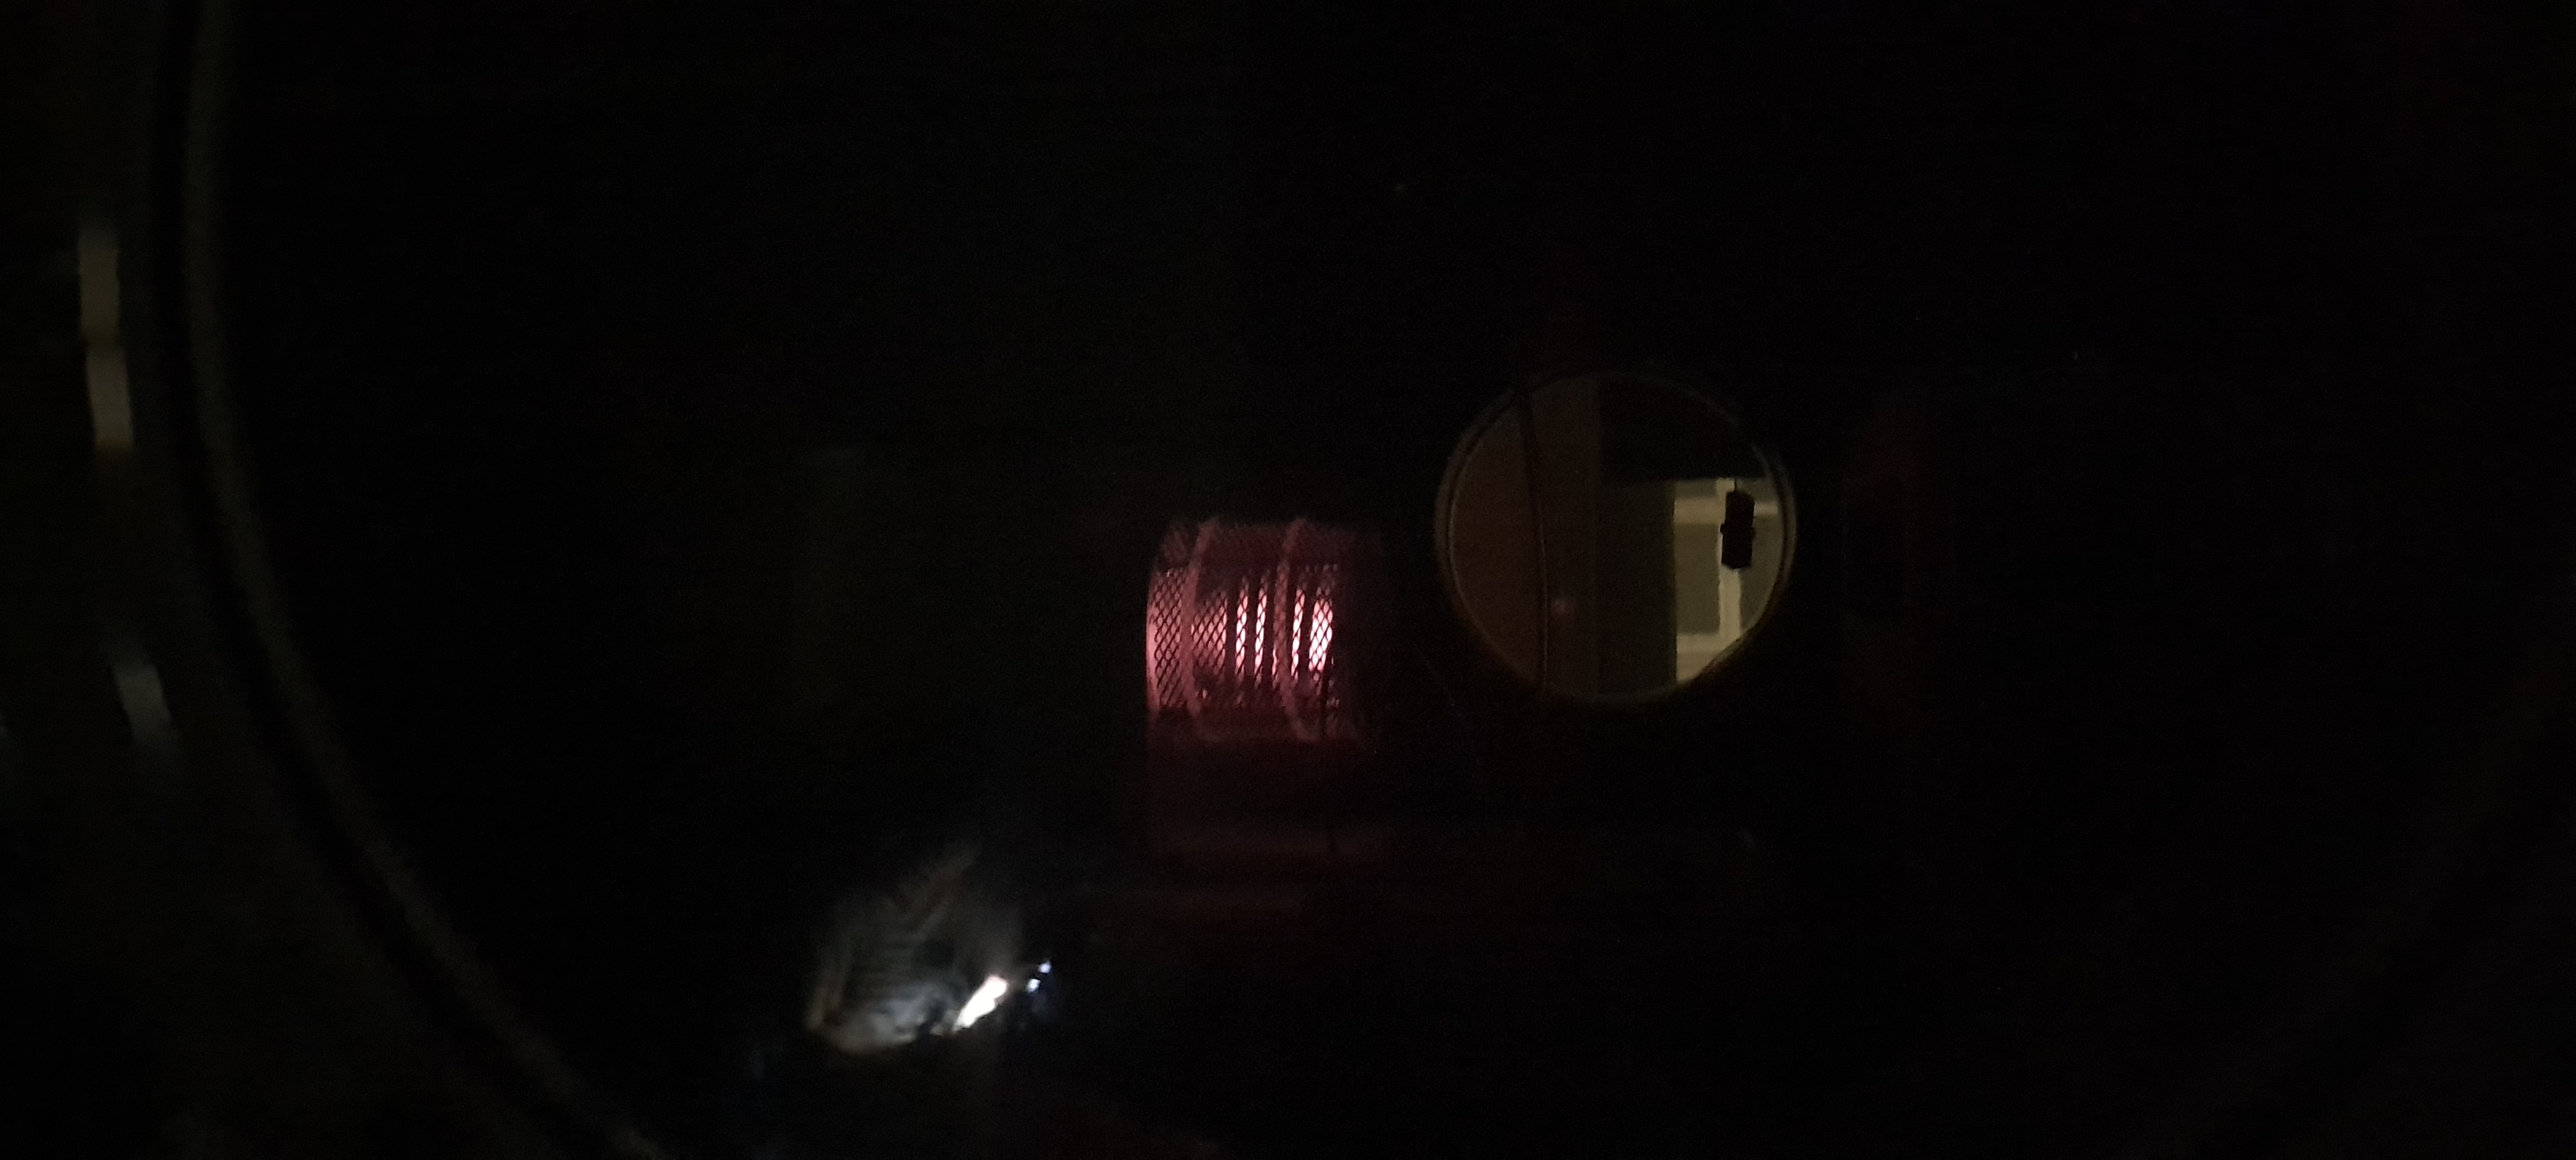
\includegraphics[width=\linewidth]{fig/deneme1/test1_ccp.jpg}
    \caption{CCP formed within the thruster during first firing test}
    \label{fig:1st_ccp}
\end{figure}

After initial ignition RF power have been increased to 30W and screen and acceleration grids have been polarized with ground and +1000V potential respectively. It has been observed that increased RF power has caused plasma to transit to inductively coupled plasma (ICP). After the grids are polarized bright flashes have been observed forming between grids and potentials of the grids have begun to fluctuate indicating that an electical arc is forming between grids. Propellant flow rate has been increased to 25 SCCM to increase the number of ions within the discharge chamber but unfortunately electical arc has continued to form. Excess propellant escaping the thruster has coupled with the RF antenna and created a dim glow within the vacuum chamber as shown in figure \ref{fig:1st_icp}.
\newpage

\begin{figure}[ht]
    \centering
    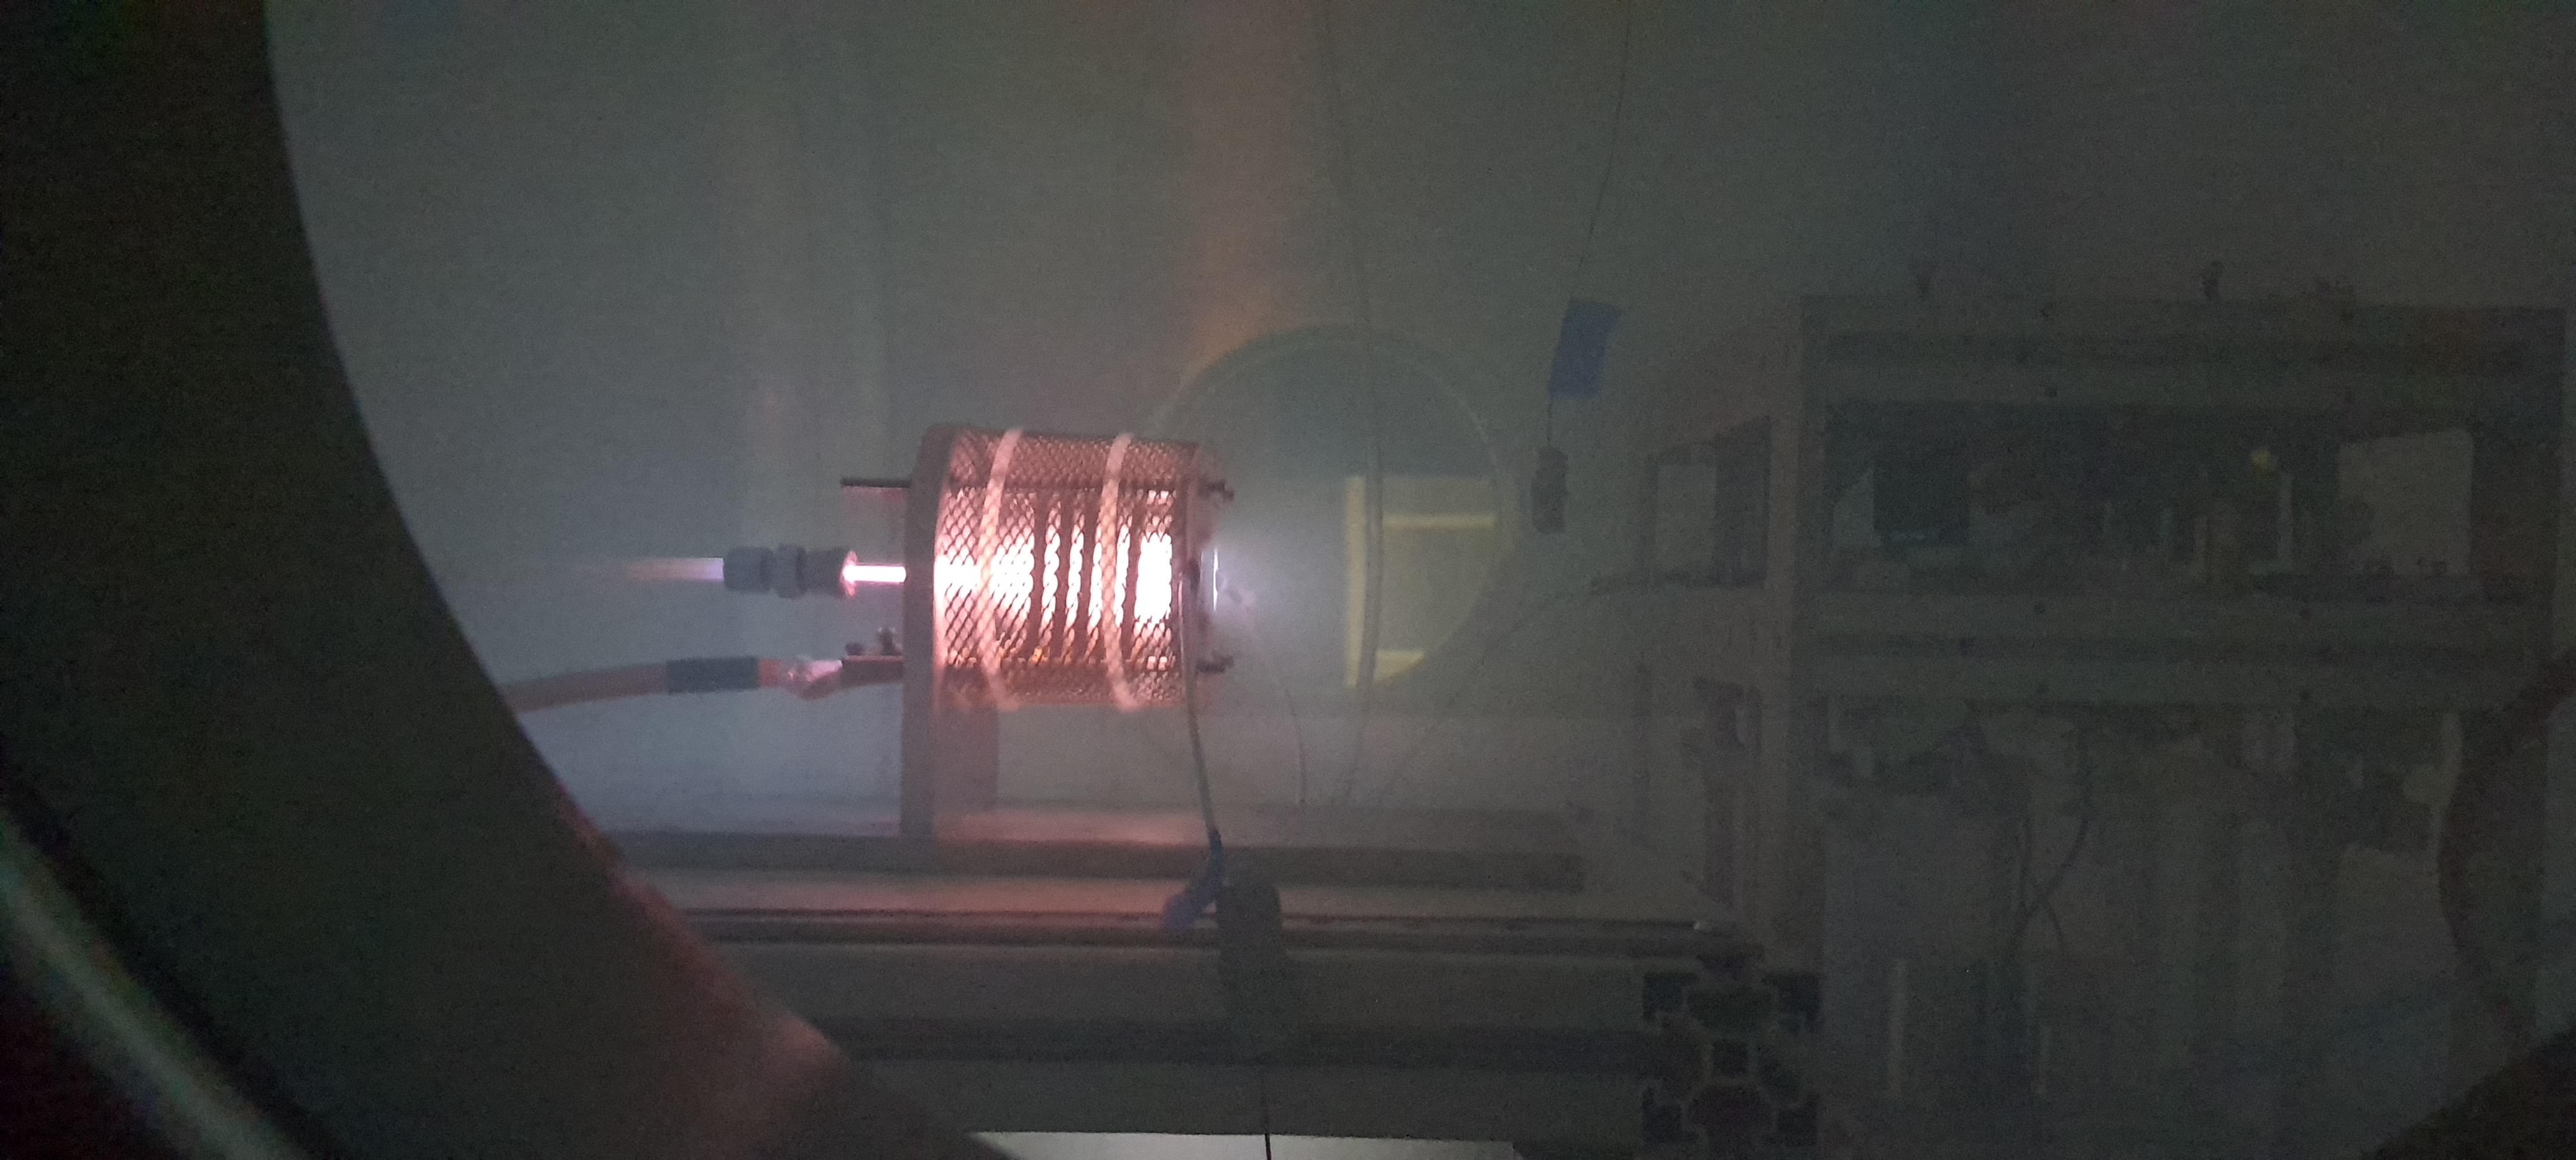
\includegraphics[width=\linewidth]{fig/deneme1/test1_discharge.jpg}
    \caption{Thruster during first firing test}
    \label{fig:1st_icp}
\end{figure}

Note that in figure \ref{fig:1st_icp} the plume exiting the thruster is not an ion beam but merely excess non-ionized propellant escaping the thruster.
At this stage test has been aborted. The failure and electical arc forming are attributed to the mechanical roughness and imperfections of the grids as shown in figure \ref{fig:1st_imperfect}. These imperfections are determined to be the result of the oxygen laser cutting process. Additionally after the test is complete the thruster is disassembled and it was discovered that a spacer plate between grids was missing due to human error. This resulted in a sub-optimal ion optics configuration.

\begin{figure}[ht]
    \centering
    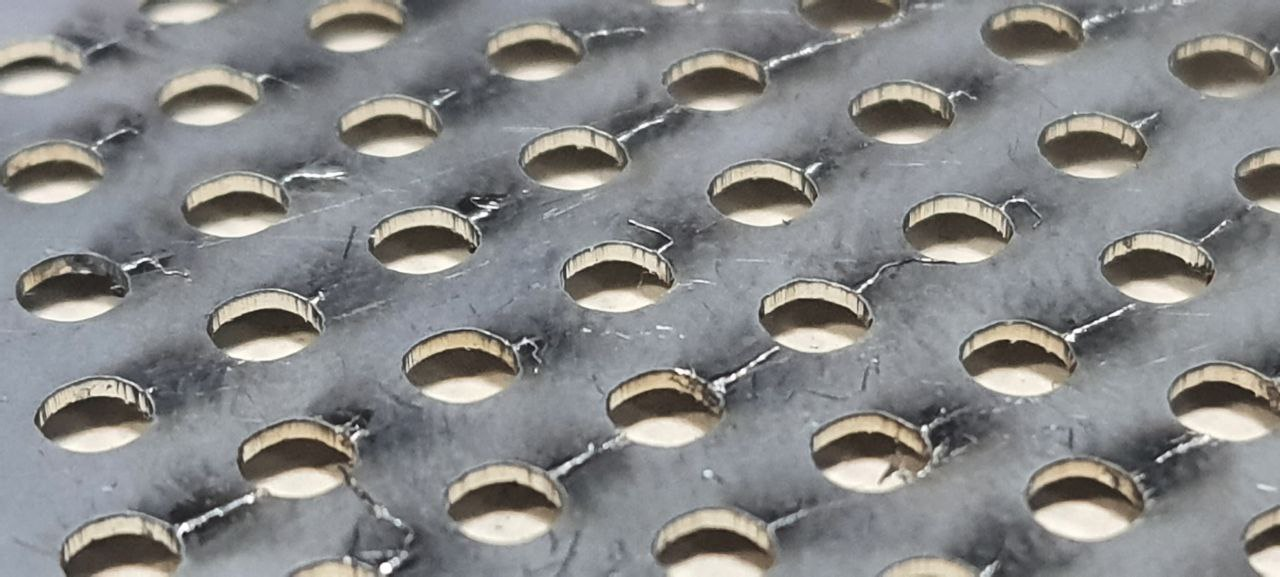
\includegraphics[scale=0.3]{fig/imperfect1.jpeg}
    \caption{Grid imperfections during first firing test}
    \label{fig:1st_imperfect}
\end{figure}

Decision has been made to remove the imperfections by hand using mechanical file prior to second firing tests.
\newpage
\subsection{Firing Test No. 2}
Before attempting to fire the thruster for the second time the ion extraction grids are extensively filed using fine sandpiper to remove roughness and imperfections. Filed grids are shown in figure \ref{fig:2nd_grids_before}. Afterwards the thruster is assembled properly with and experimental setup has been completed as described earlier. 

\begin{figure}[ht]
    \centering
    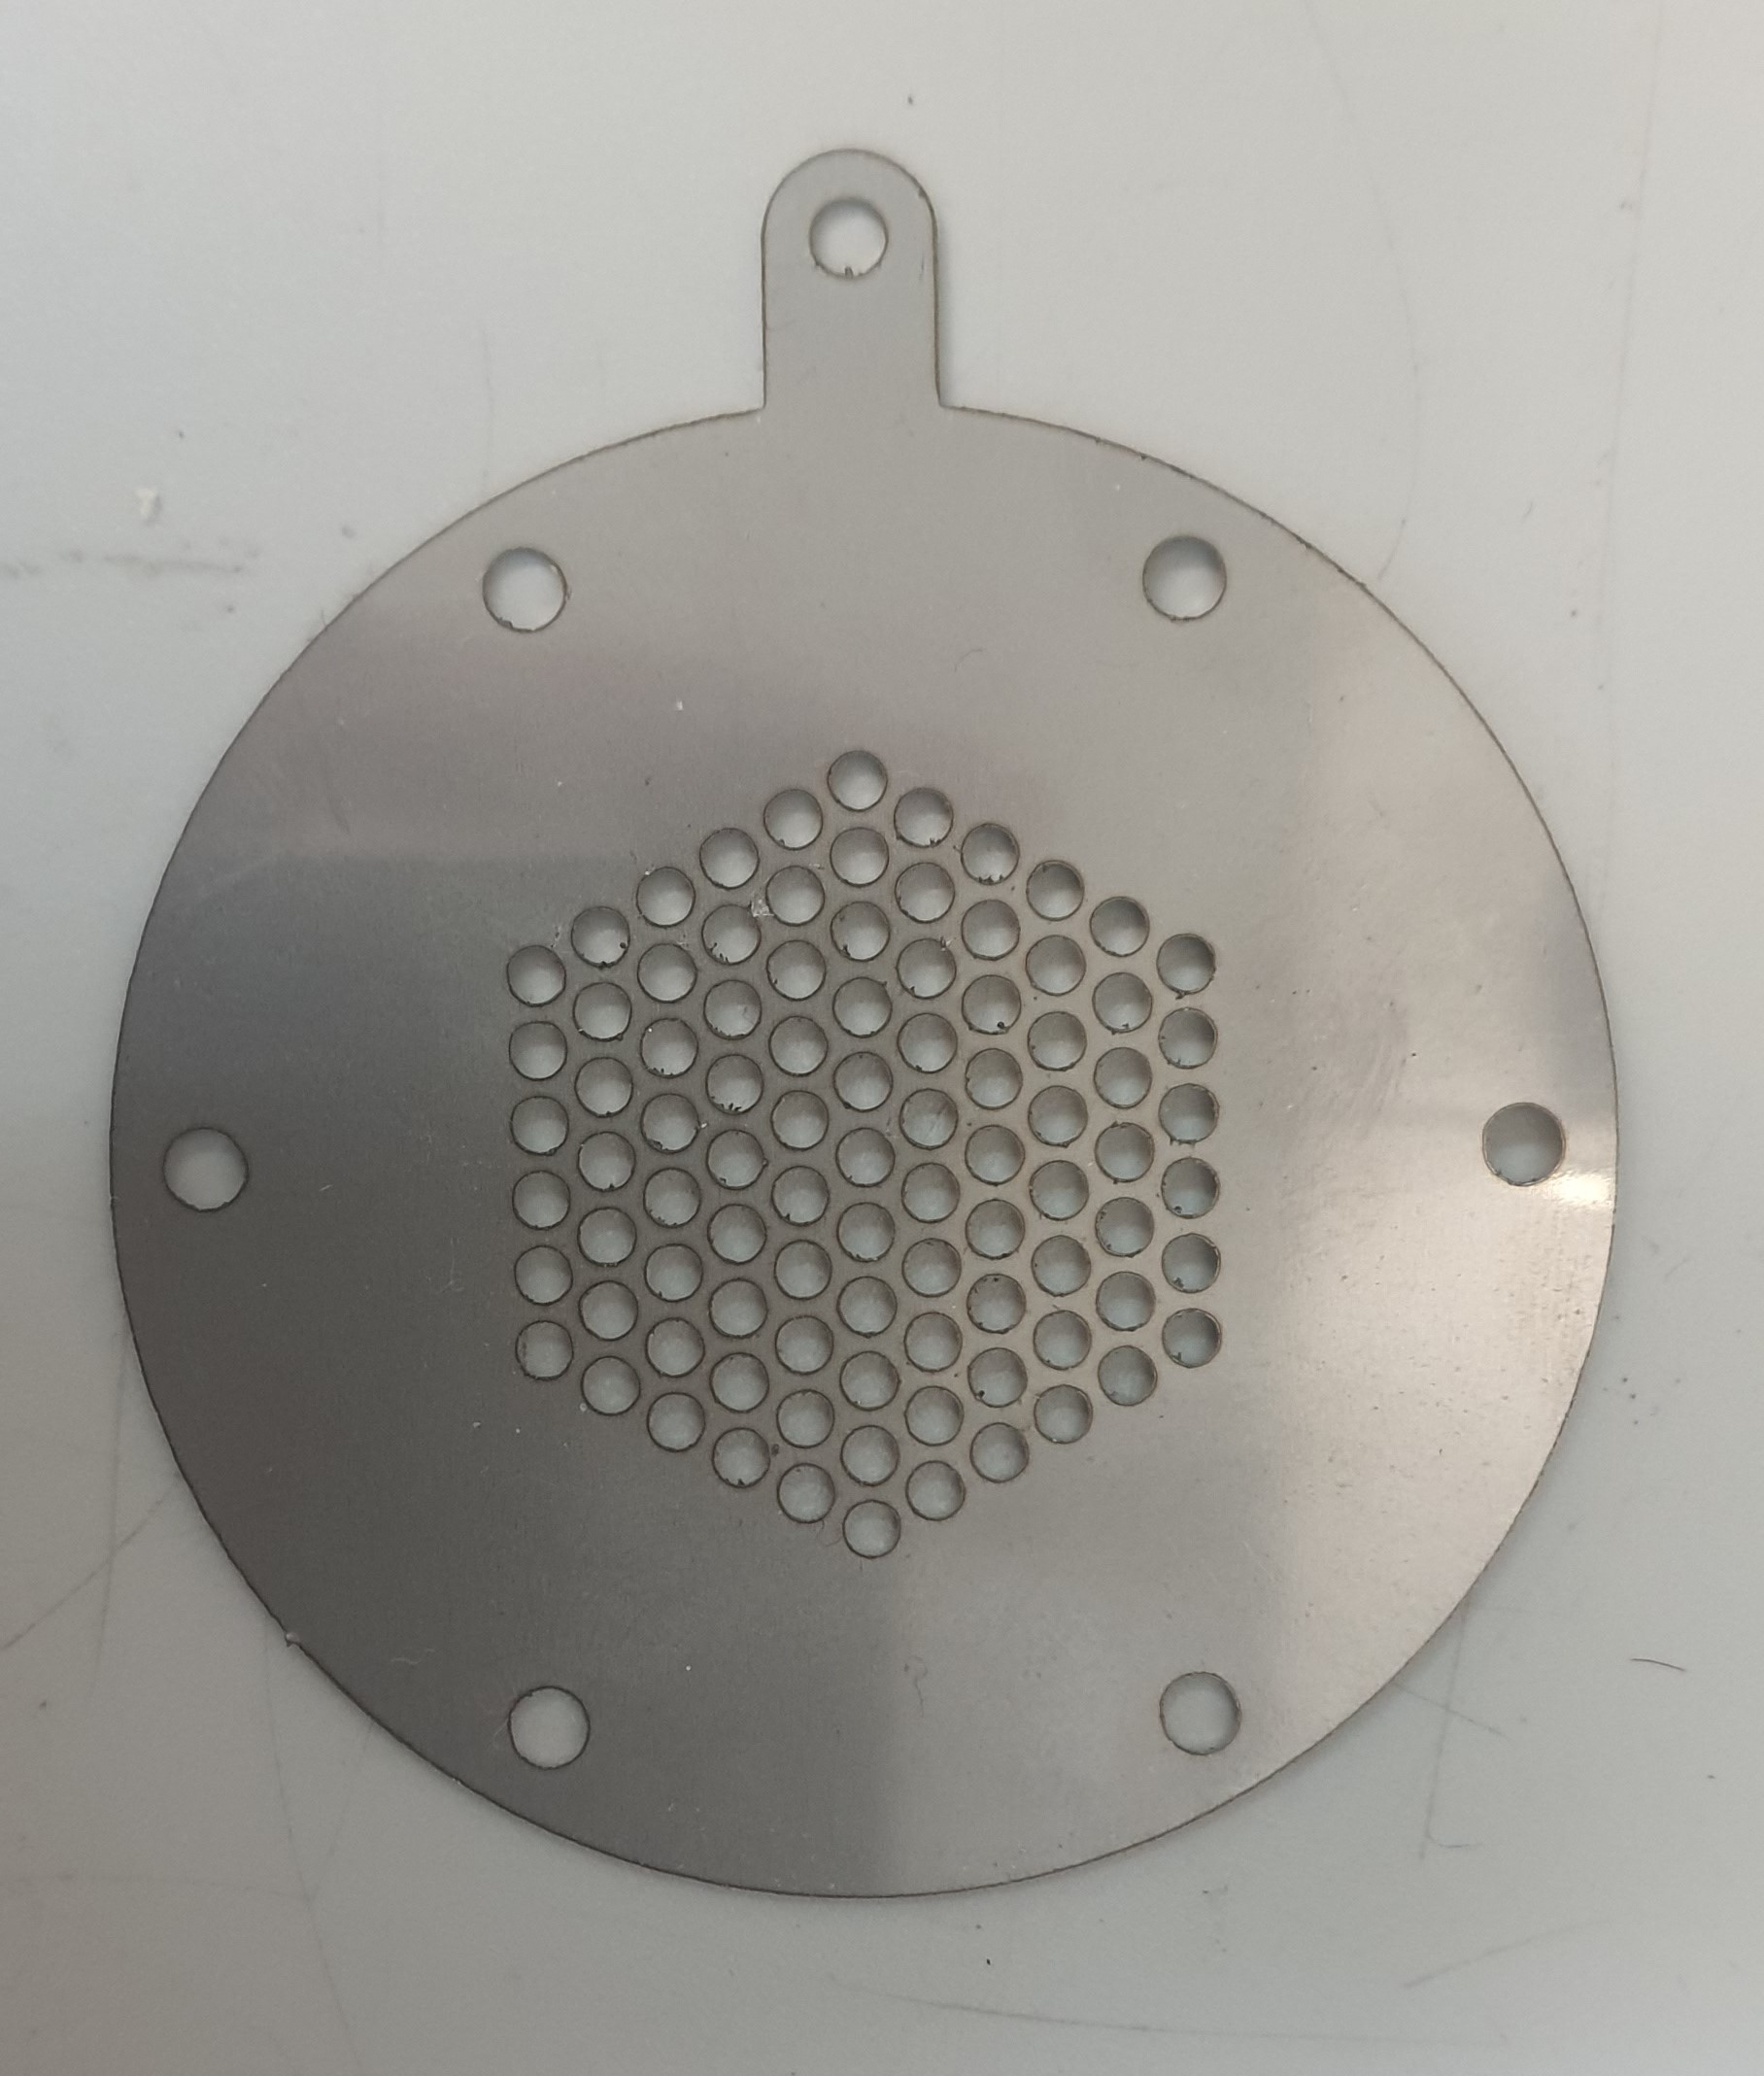
\includegraphics[width=0.4\linewidth]{fig/deneme2/test2_screen_before.jpg}
    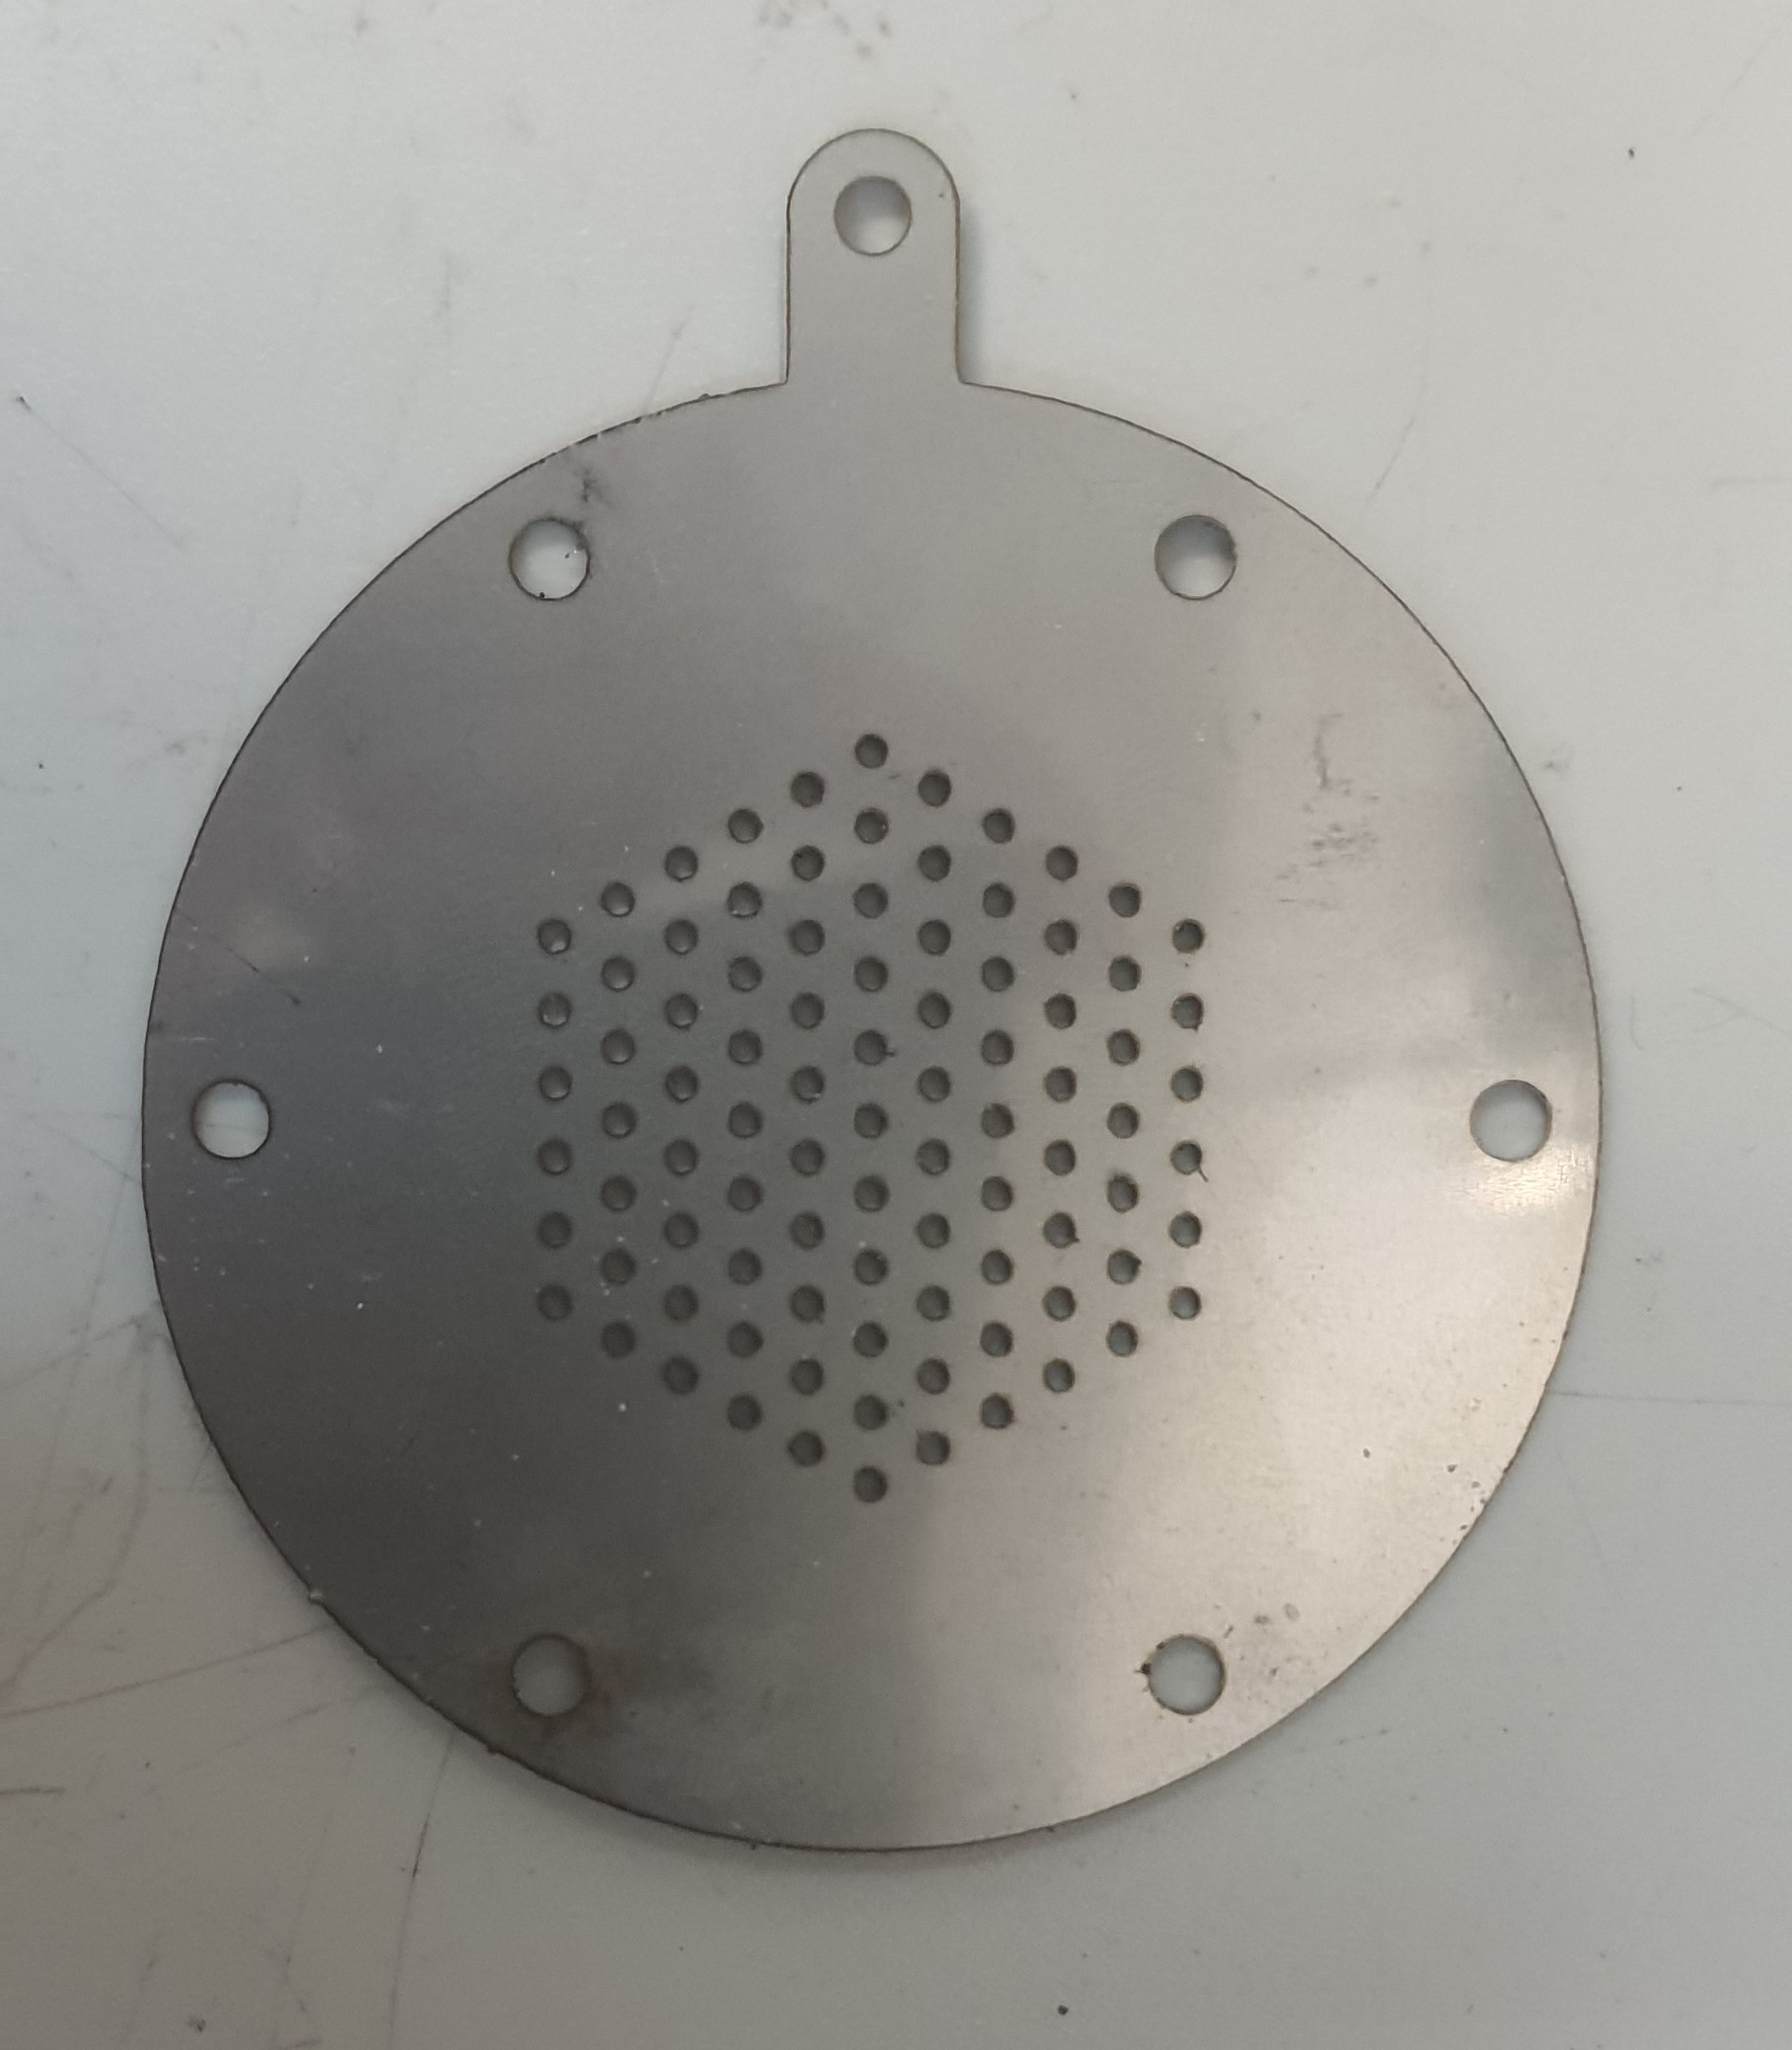
\includegraphics[width=0.41\linewidth]{fig/deneme2/test2_accel_before.jpg}
    \caption{Screen(\textit{left}) and acceleration(\textit{right}) grids before second firing test}
    \label{fig:2nd_grids_before}
\end{figure}

Prior to test the pressure level of the vacuum chamber has been reduced to $2.39x10^{-4}$ torrs. Similar to first firing test plasma has been succesfully ignited as CCP with 5W of RF power and 13 SCCM propellant flow rate. RF power level has been steadily increased to 45W and ICP has been achieved as shown in figure \ref{fig:2nd_icp}. 

\begin{figure}[ht]
    \centering
    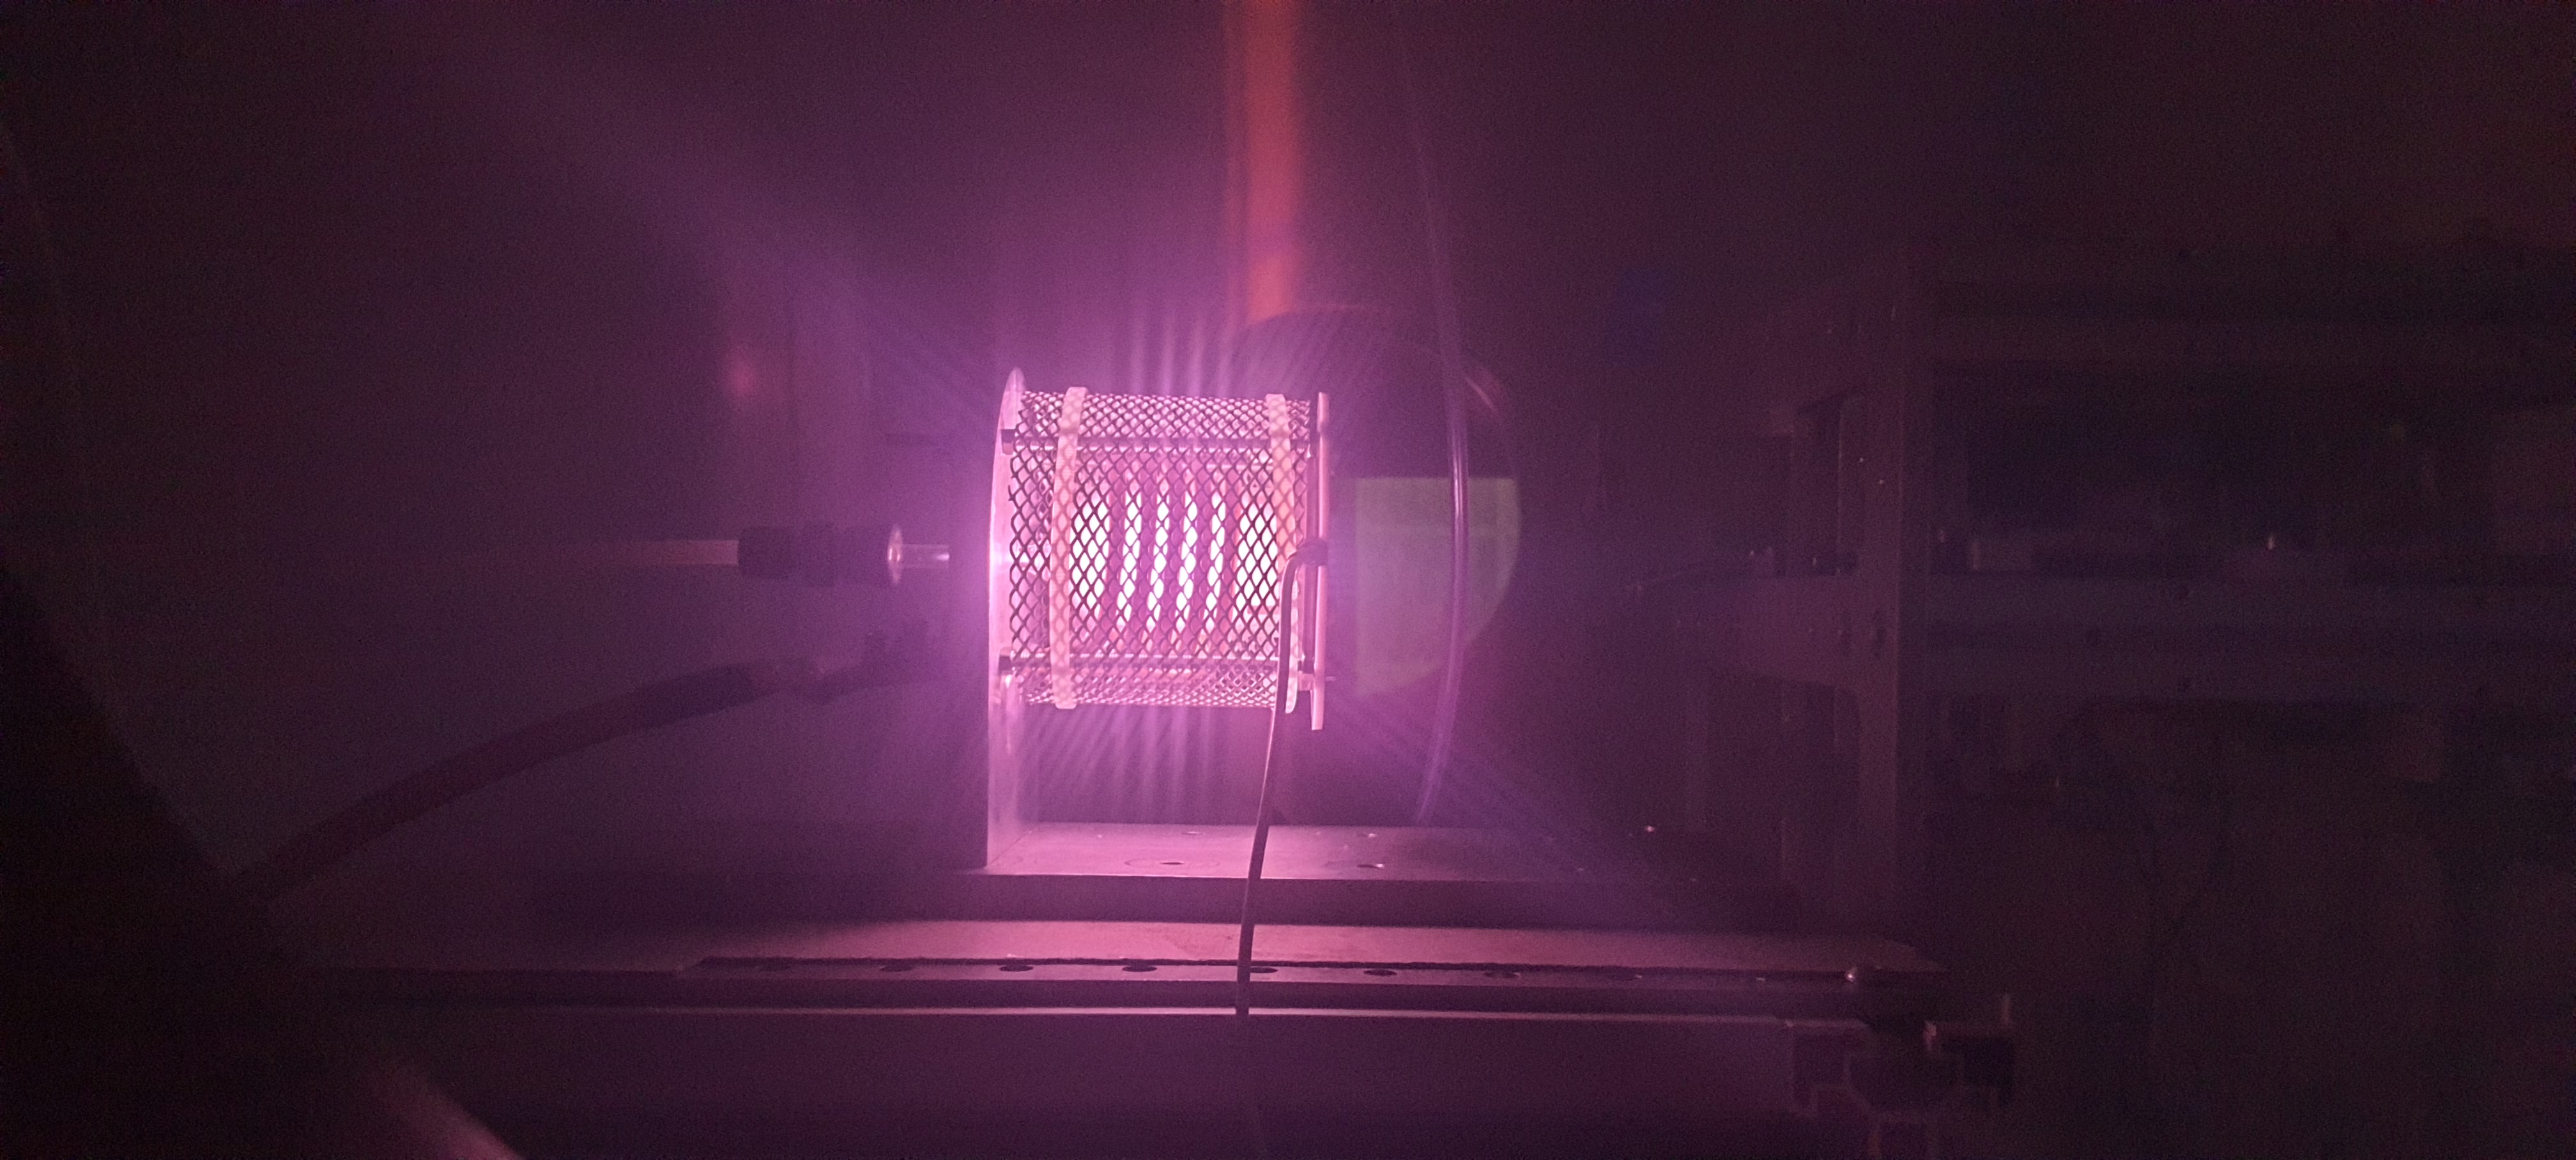
\includegraphics[width=\linewidth]{fig/deneme2/test2_icpglow.jpg}
    \caption{ICP during second firing test}
    \label{fig:2nd_icp}
\end{figure}

After ICP is acquired the screen and acceleration grids have been polarized with ground and +600V of potential respectively. It was observed that despite extensive mechanical filing impurities of grids continued to cause electrical short between grids. In figure \ref{fig:2nd_short} a bright flash can be seen due to forming of electrical arcs. 

\begin{figure}[ht]
    \centering
    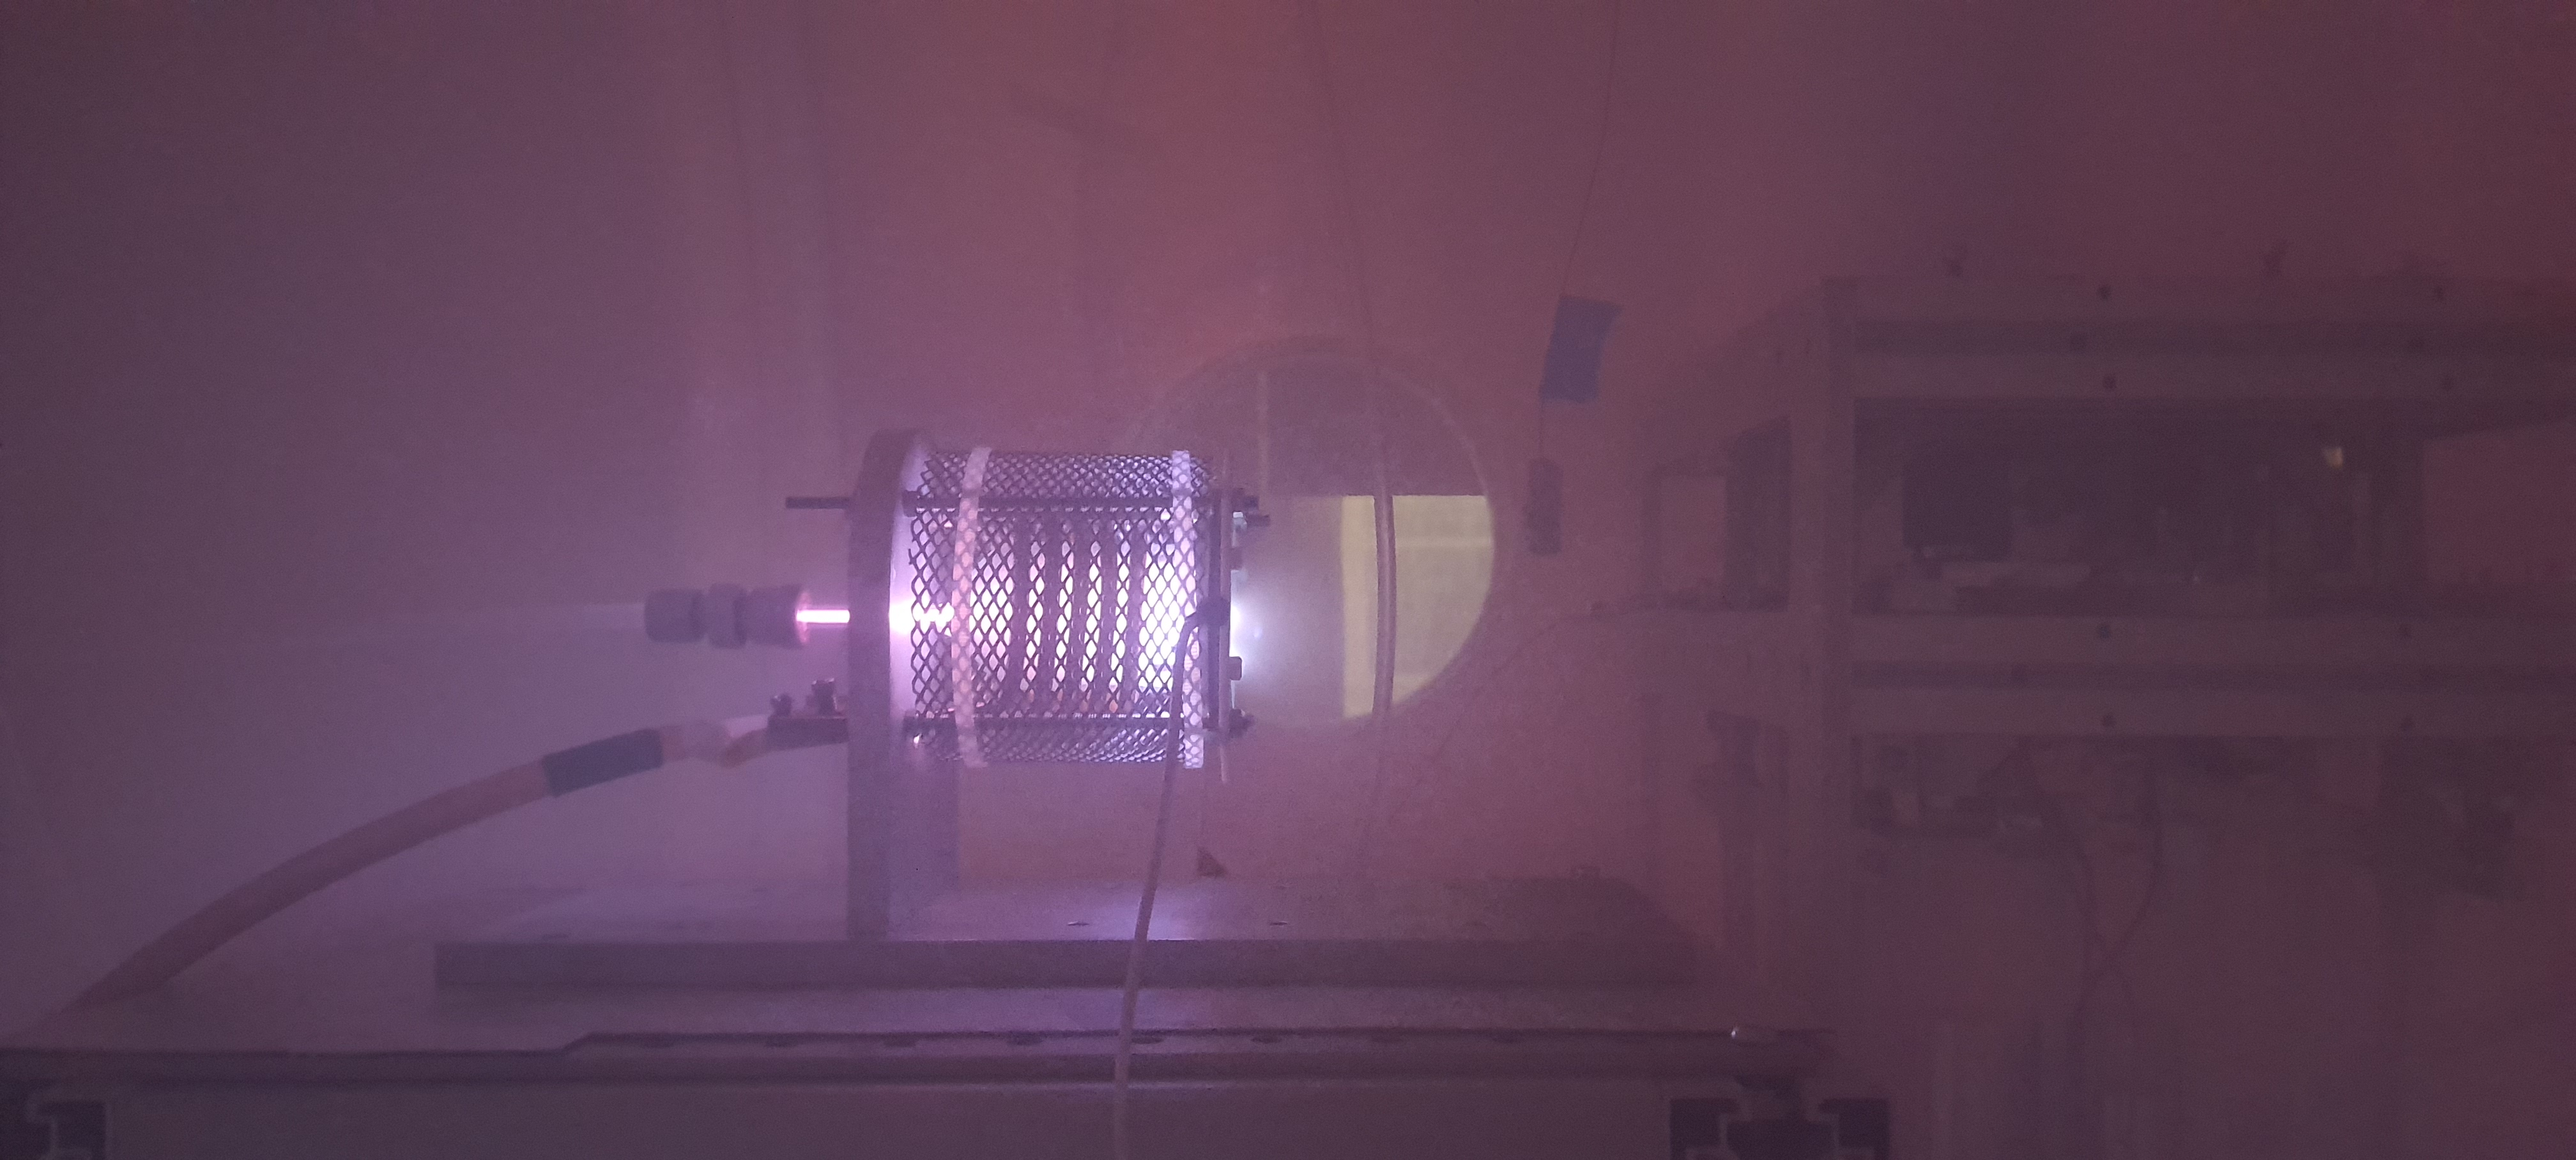
\includegraphics[width=\linewidth]{fig/deneme2/test2_short.jpg}
    \caption{Electrical short during second firing test}
    \label{fig:2nd_short}
\end{figure}

The test has been aborted at this point. After disassembling the thruster severe degragation of ion accelerator grids has been discovered as shown in figure \ref{fig:2nd_grids_after}.

\begin{figure}[ht]
    \centering
    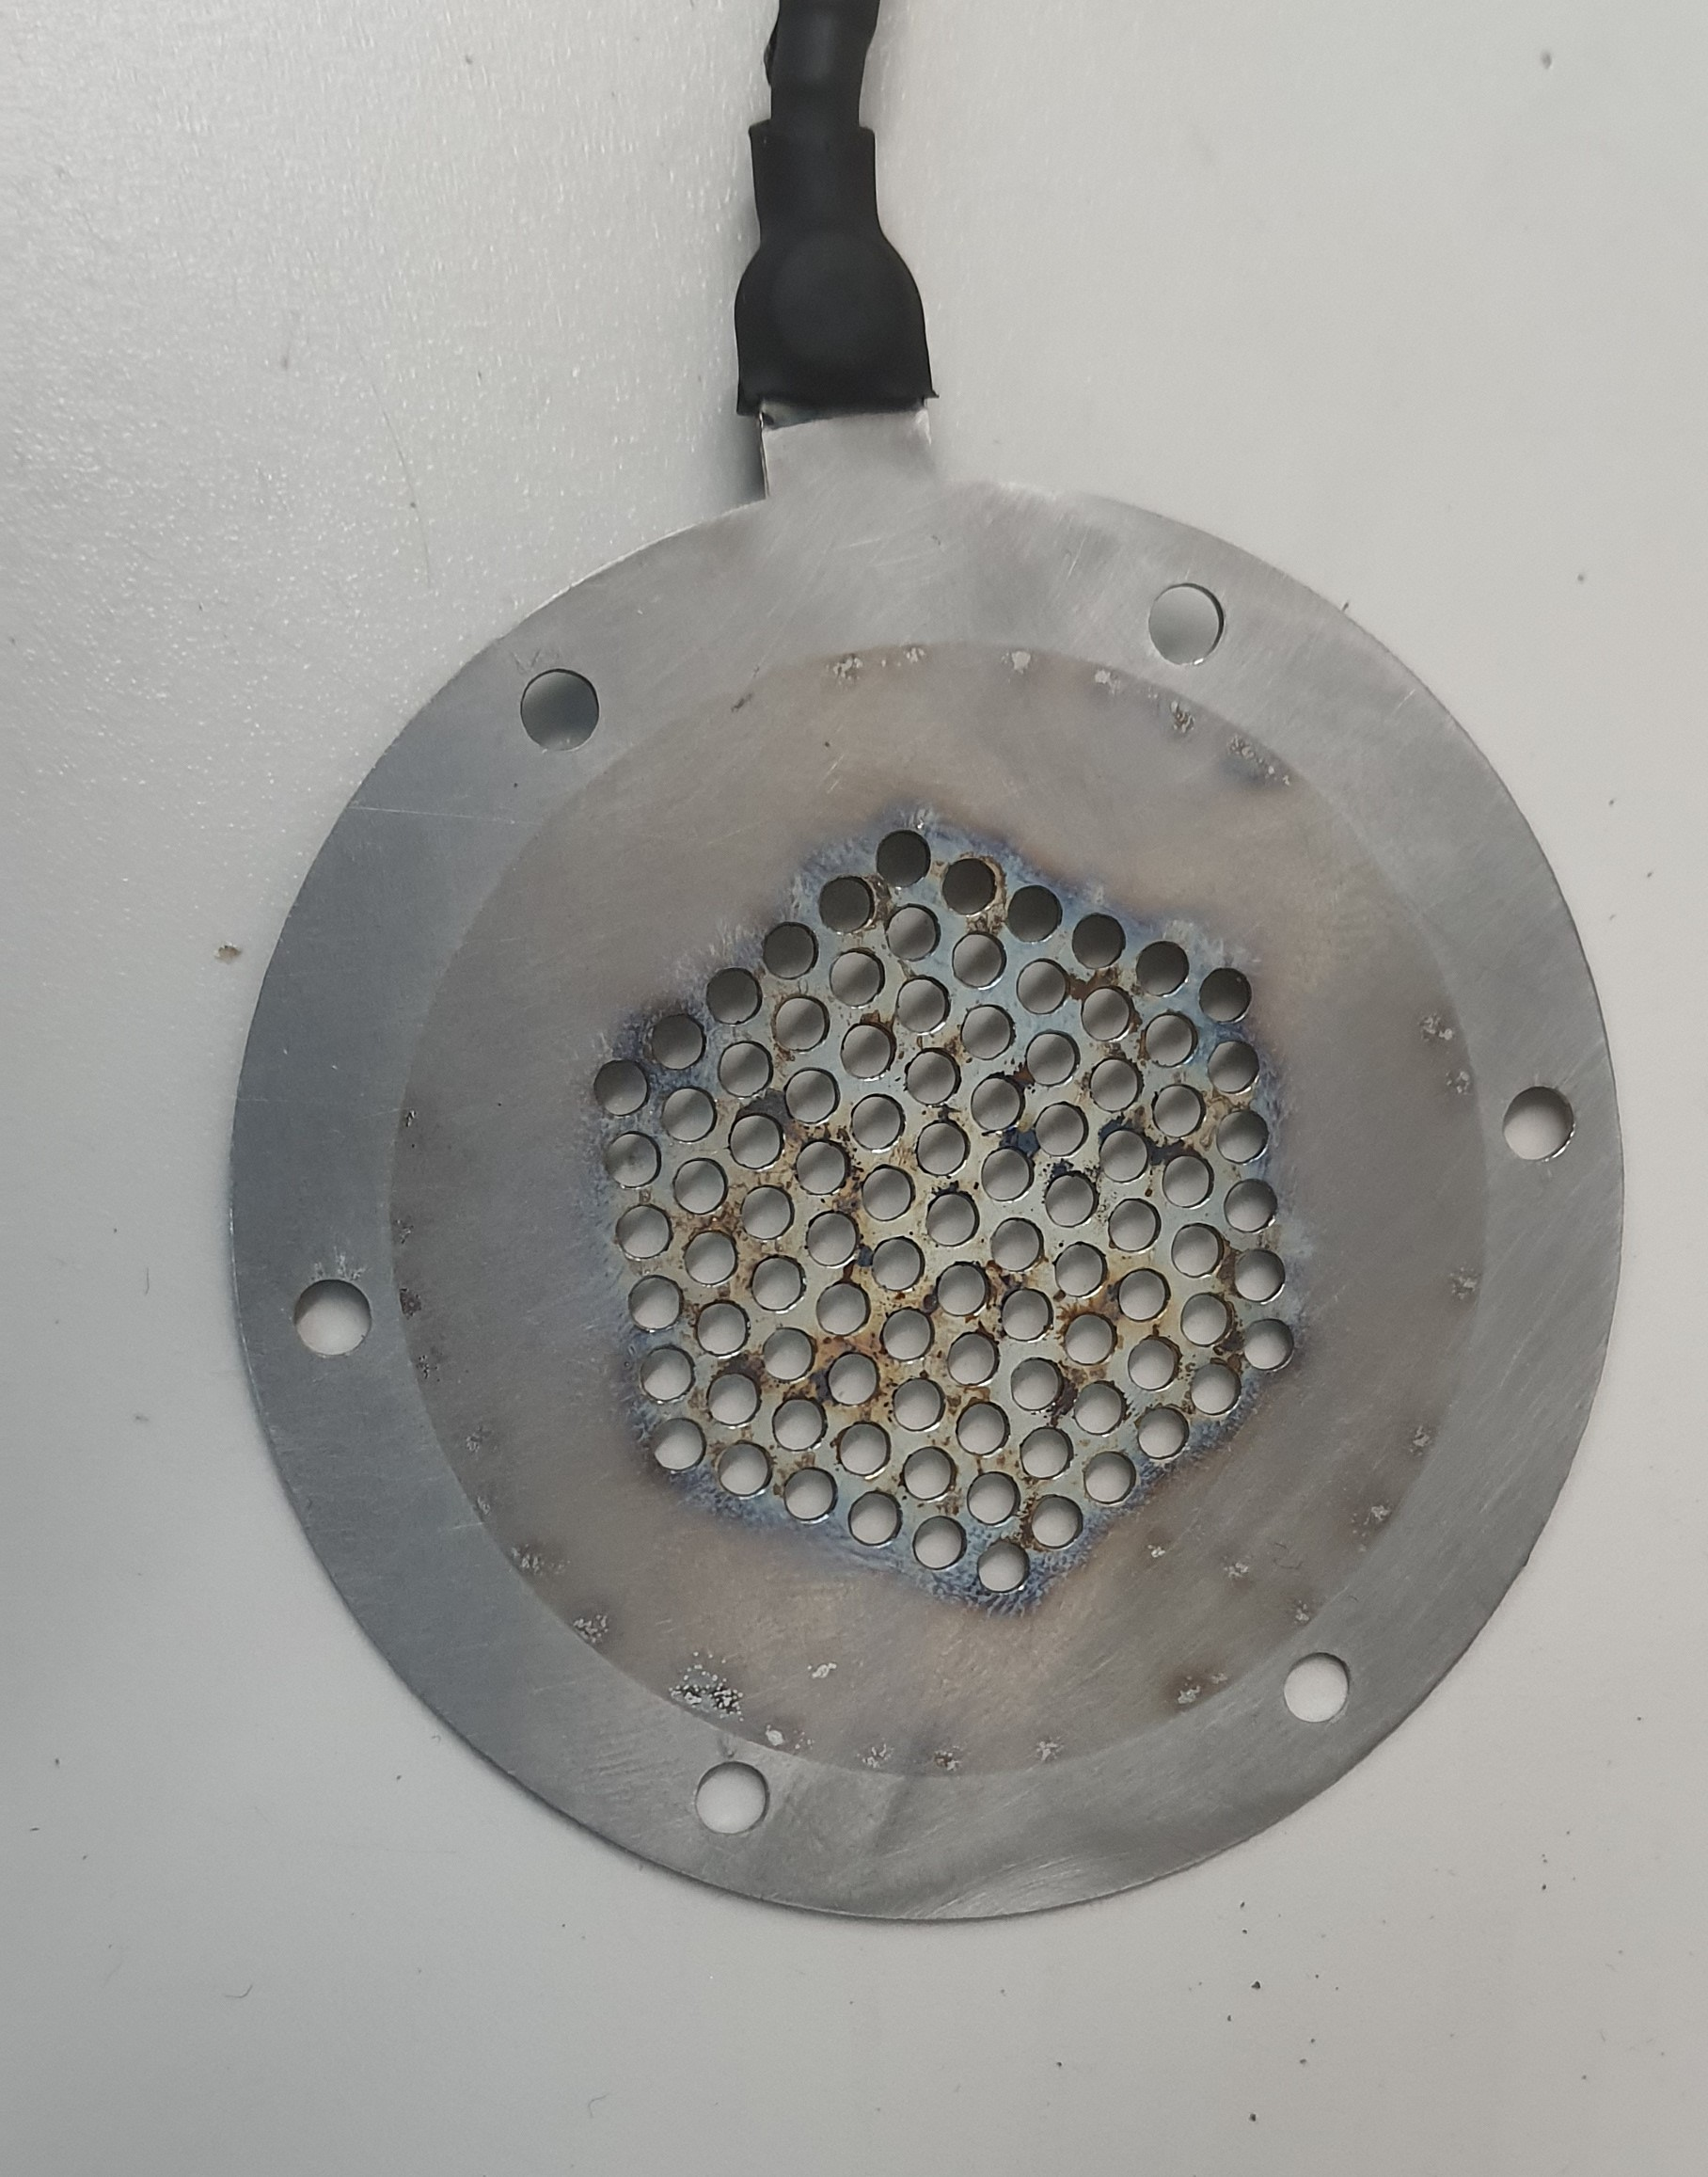
\includegraphics[width=0.41\linewidth]{fig/deneme2/test2_screen_after.jpg}
    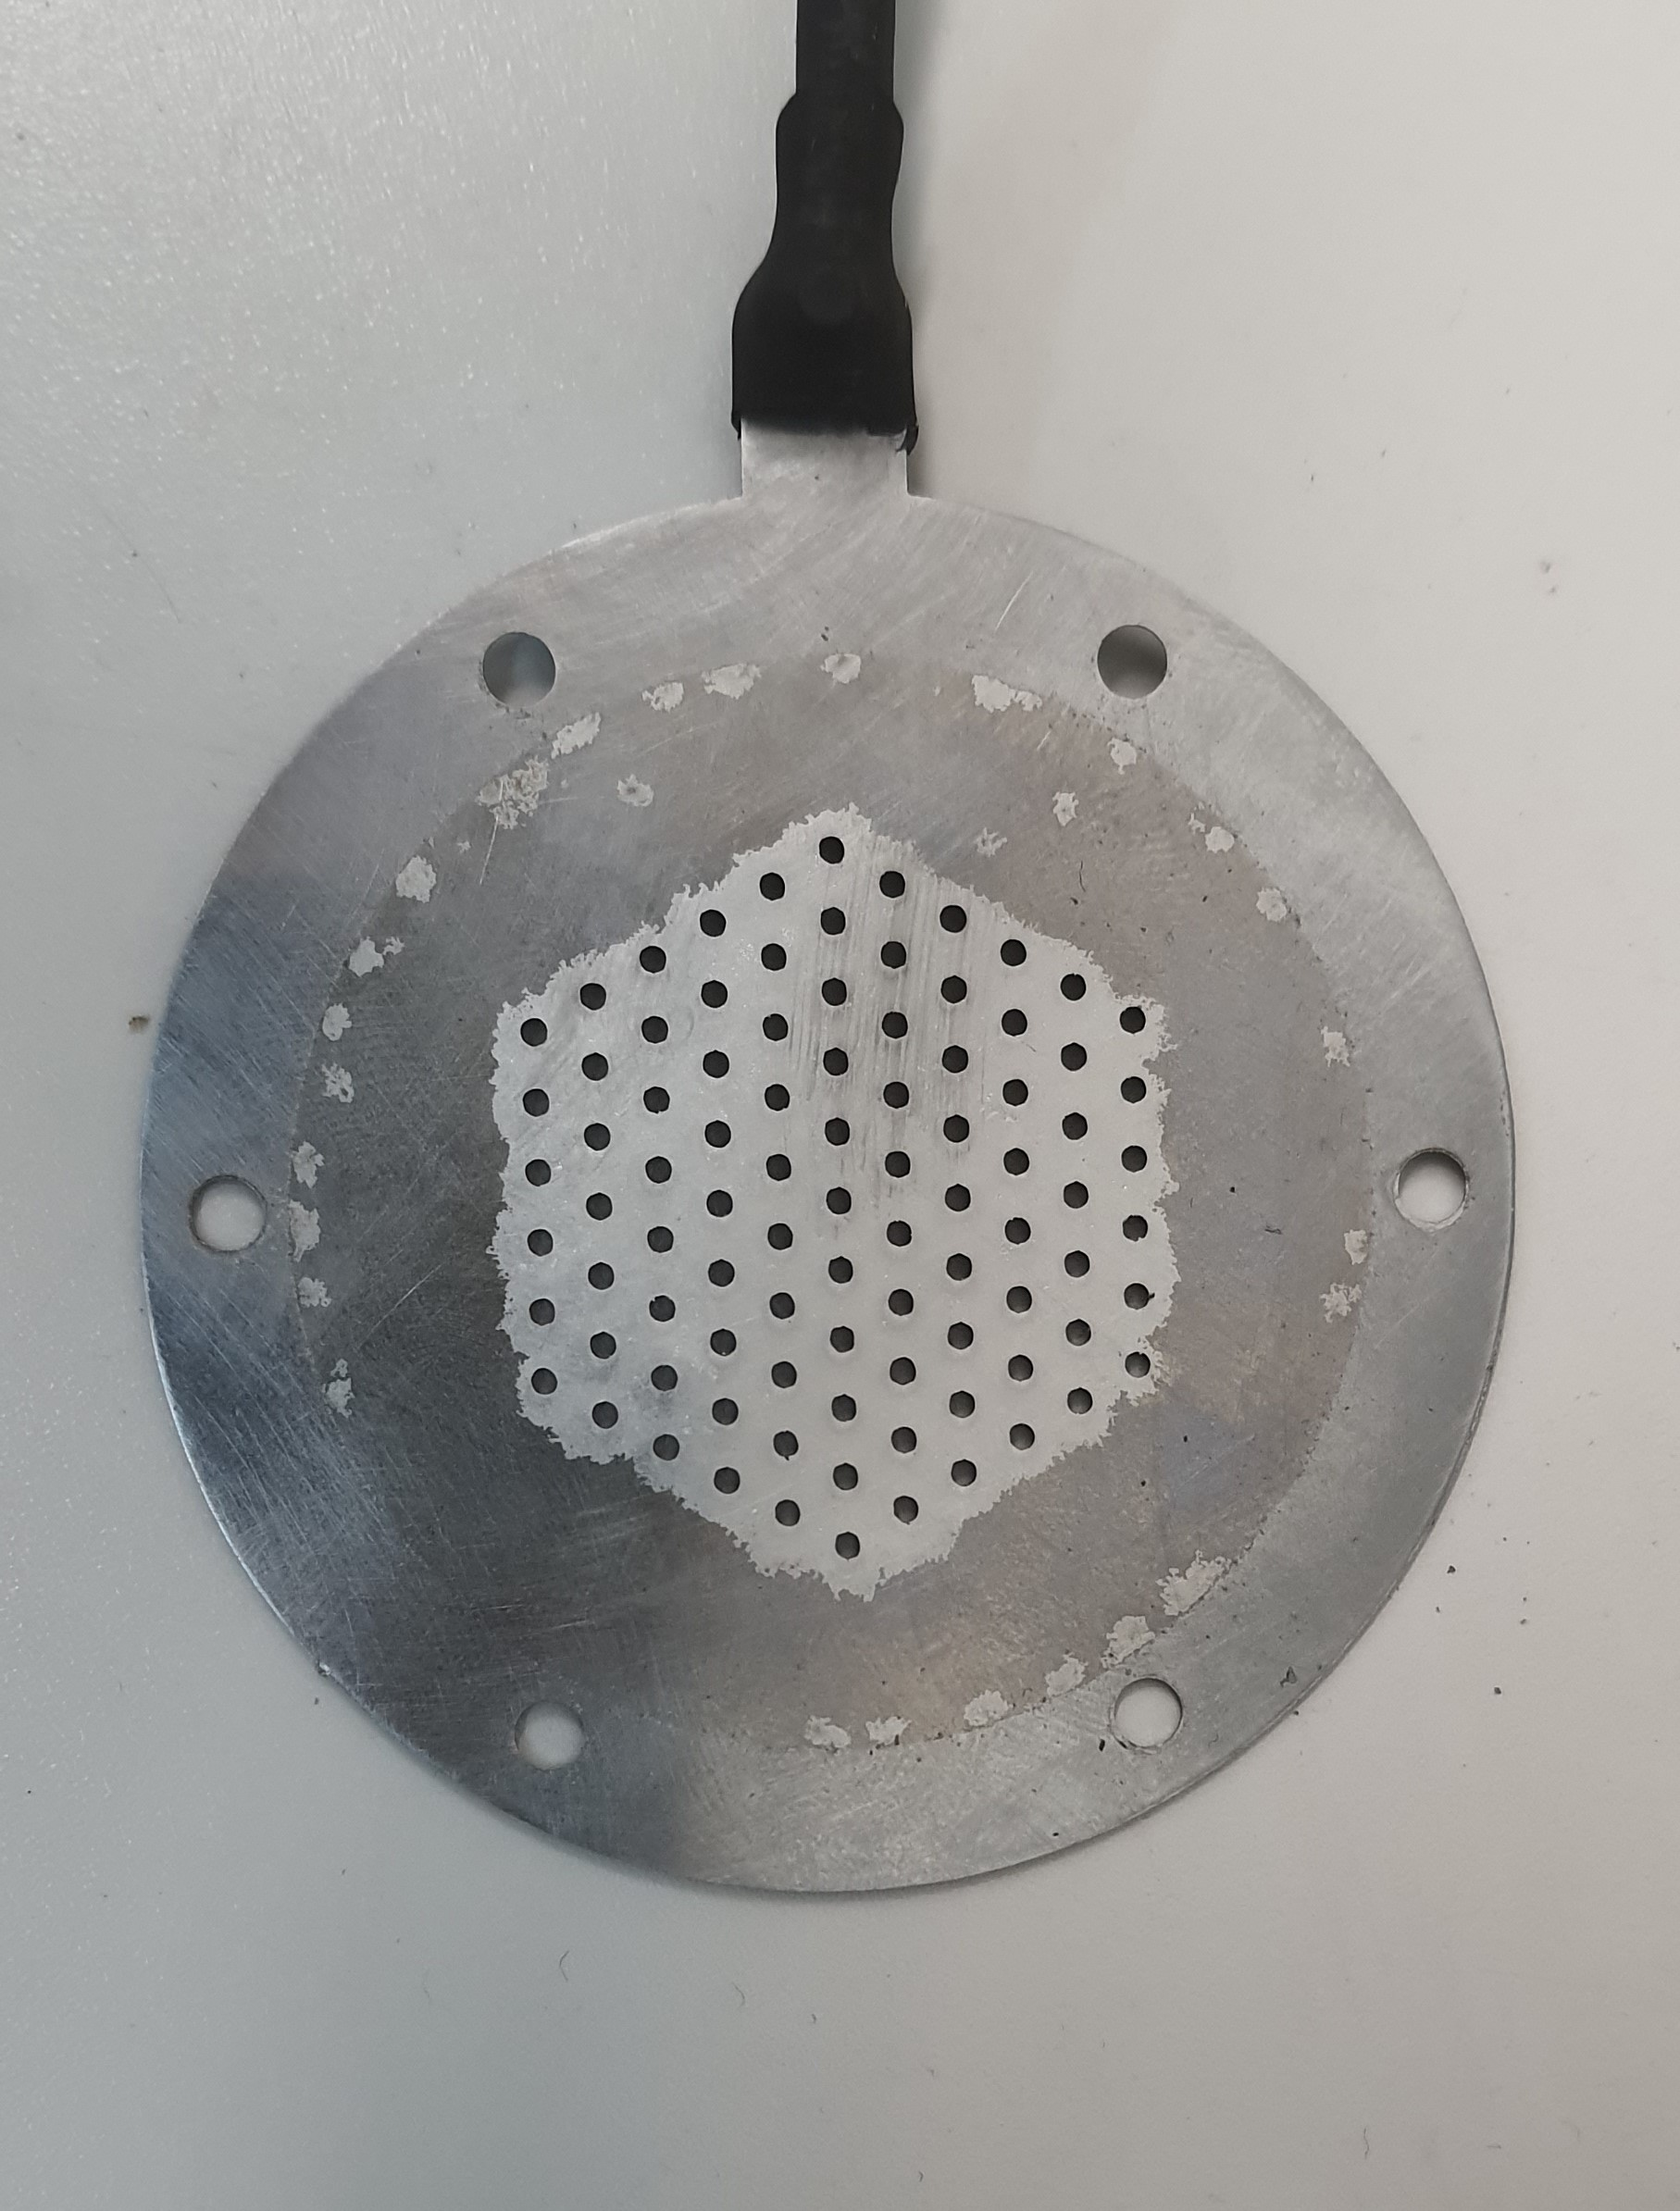
\includegraphics[width=0.4\linewidth]{fig/deneme2/test2_accel_after.jpg}
    \caption{Screen(\textit{left}) and acceleration(\textit{right}) grids after second firing test}
    \label{fig:2nd_grids_after}
\end{figure}

\newpage
\subsection{Firing Test No. 3}
For third attempt a new set of grids with increased center to center distance between apertures have been designed and manufactured. Manufacturing process was again oxygen laser cutting. Center to center distance have been increased to 4.2mm for third firing test. This resulted the number of apertures to decrease from 91 to 61. Areas around the apertures have been filed using DRAMEL device. Grids after filing are shown in figure \ref{fig:3rd_grids_before}.

\begin{figure}[ht]
    \centering
    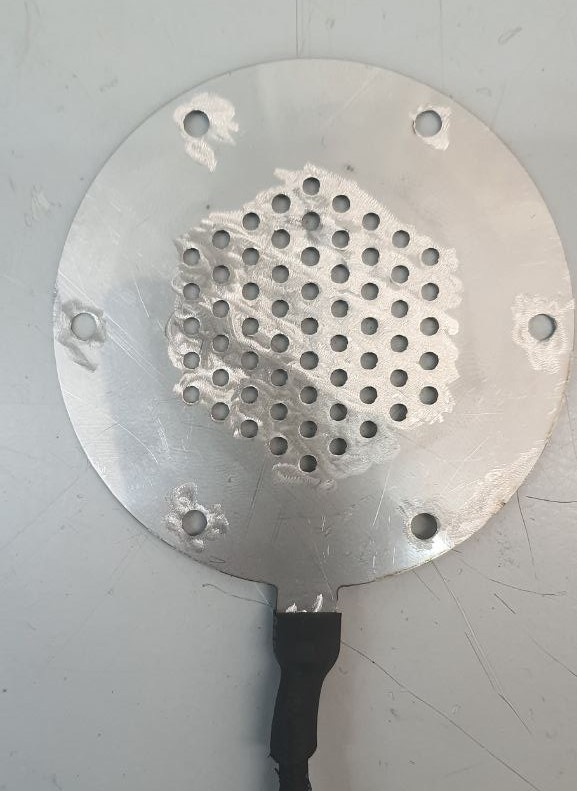
\includegraphics[width=0.41\linewidth]{fig/deneme3/test3_screen_before.jpeg}
    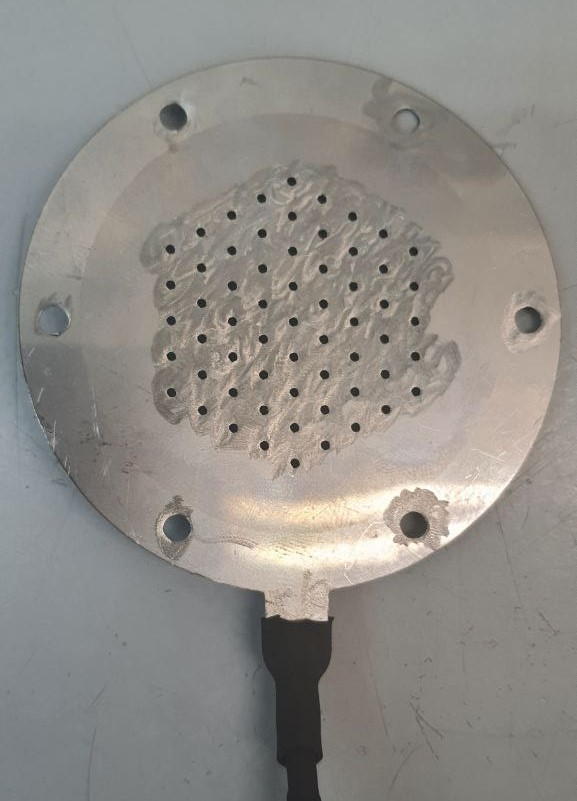
\includegraphics[width=0.4\linewidth]{fig/deneme3/test3_accel_before.jpeg}
    \caption{Screen(\textit{left}) and acceleration(\textit{right}) grids used in third firing test}
    \label{fig:3rd_grids_before}
\end{figure}

Purpose of this change in aperture center to center distance is to keep arcs from forming between apertures. Thruster is assembled and experimental setup has been established normally. During the test the pressure level inside vacuum chamber has been reduceed to $1.34x10^{-4}$ torrs. RF input power and propellant flow rate have been set to 30W and 12 SCCM respectively.     
Screen grid and acceleration grid have been polarized with ground and -600V respectively. Plasma inside the thruster has transited to ICP at approximately 60W of RF power. 
Despite increased center to center distance between apertures and even extensive filing electrical arcs have been observed to continue forming. Test has been aborted. It was decided to seek alternate methods for grid production in order to completely eliminate burrs and impurities during manufacturing process. 
\newpage
\subsection{Firing Tets No. 4}
A new set of grids have been manufactured. This time nitrogen was used during laser cutting. Grid materal have also been changed. Instead of SS304, SS316 grade steel was used for the fourth test. These changes resulted in a much more robust and smooth ion extractor grids as shown in figure \ref{fig:4th_grids_before}. 

\begin{figure}[ht]
    \centering
    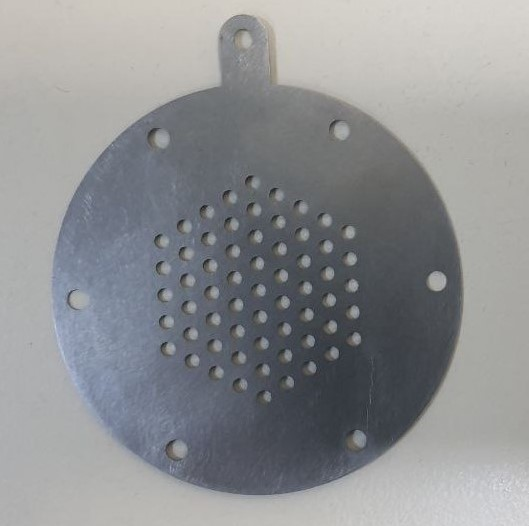
\includegraphics[width=0.41\linewidth]{fig/deneme4/test4_screen_before.jpg}
    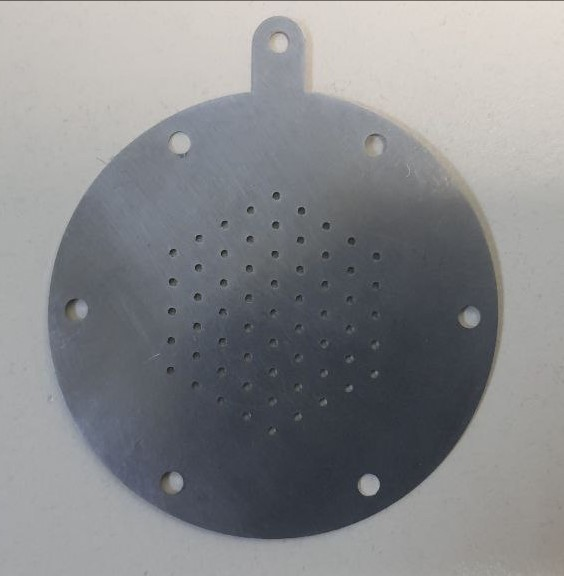
\includegraphics[width=0.4\linewidth]{fig/deneme4/test4_accel_before.jpg}
    \caption{Screen(\textit{left}) and acceleration(\textit{right}) grids before in fourth firing test}
    \label{fig:4th_grids_before}
\end{figure}

RF power has been set to 10W and propellant flow rate was set 13 SCCM. Plasma ignition was succesfully achieved in CCP. RF power has been increased gradually until ICP is acheieved as shown in figure \ref{fig:4th_icp}. Transition from CCP to ICP has occured around 80W which is the highest level at which the ICP has been achieved so far. 

\begin{figure}[ht]
    \centering
    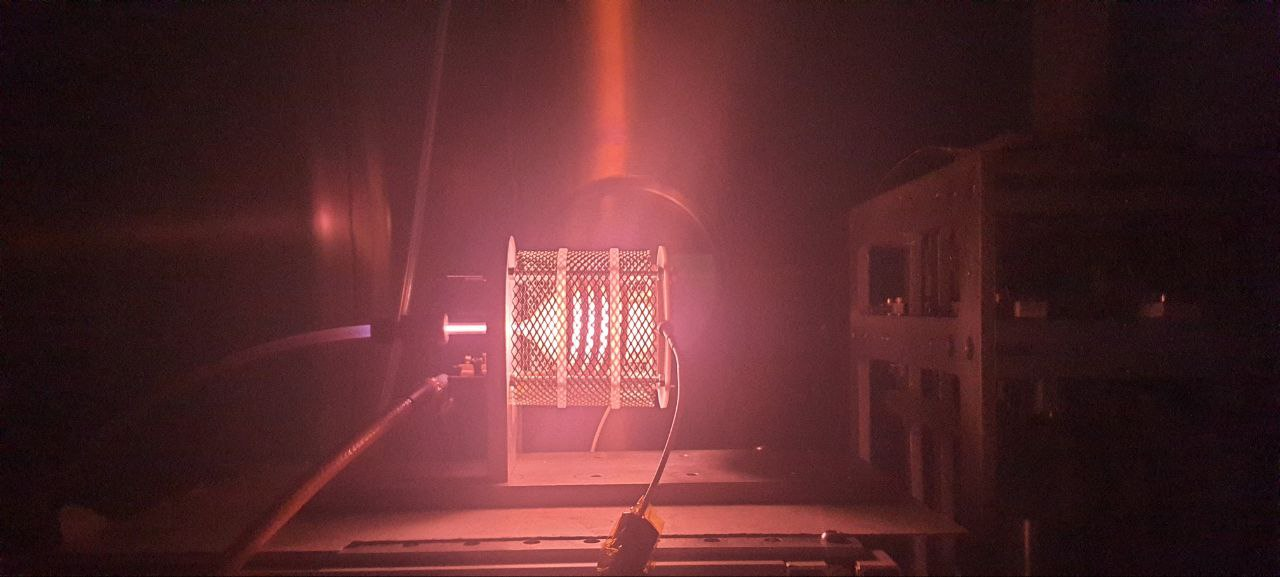
\includegraphics[width=\linewidth]{fig/deneme4/test4_icp.jpeg}
    \caption{ICP during fourth firing test}
    \label{fig:4th_icp}
\end{figure}

Initally screen and acceleration grid potentials were set to +1000V and ground potential respectively. This configuration yielded no ions and introduced slight arcing. Potentials were changed to +600V for screen grid and -200V. This change still yielded no accelerated ions but reduced the occurence frequency of arcs. Afterwards screen grid potential was increased to +800V while acceleration grid potential was kept at -200V. Under this configuration forming of a single beamlet from one of the apertures was observed as shown in 
figure \ref{fig:4th_single}.
\begin{figure}[ht]
    \centering
    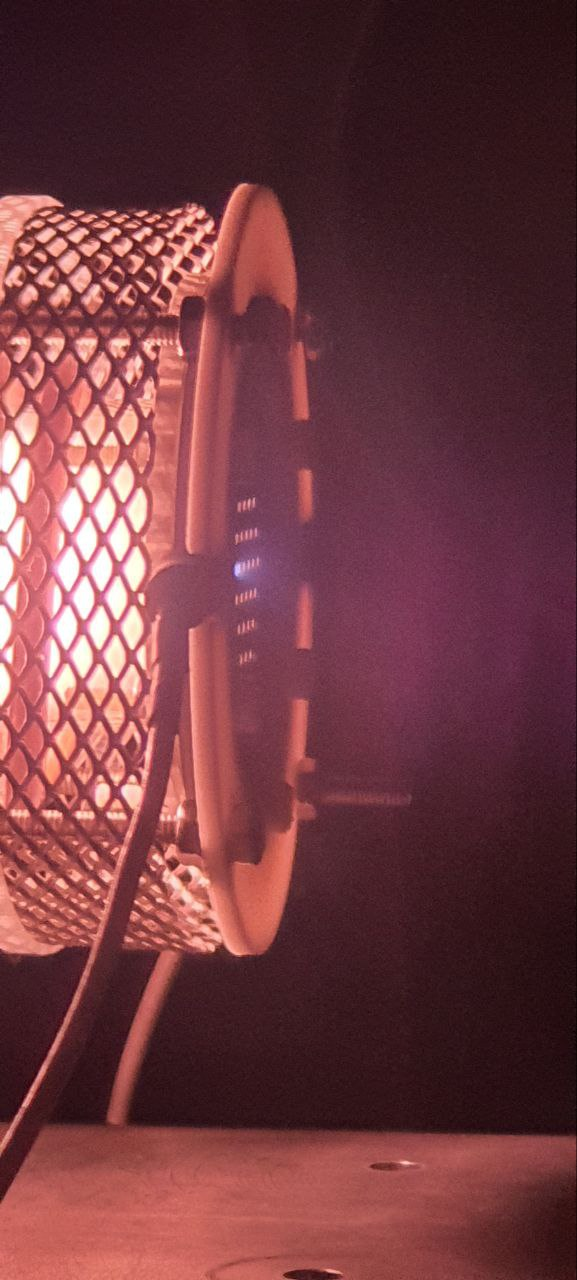
\includegraphics[scale=0.4]{fig/deneme4/test4_singlebeam.jpeg}
    \caption{Single ion beam forming}
    \label{fig:4th_single}
\end{figure}

At this point it was concluded that the arcing problem between grids was resolved. RF power has been increased to 120W and ion beams from the rest of the apertures have been observed to form as shown in figure \ref{fig:4th_multi}. 

\begin{figure}[ht]
    \centering
    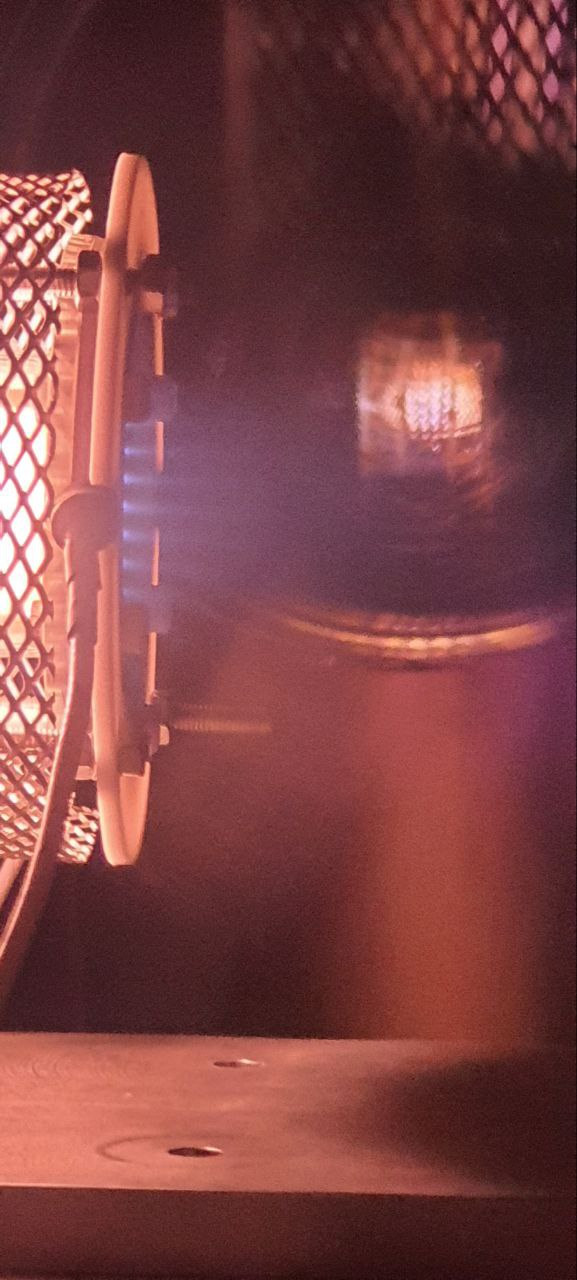
\includegraphics[scale=0.4]{fig/deneme4/test4_multibeam.jpeg}
    \caption{Multiple ion beam forming}
    \label{fig:4th_multi}
\end{figure}

This stage marks the first proper successful ion acceleration and discharge. Changing experimental parameters; RF power, flow rate, grid potentials offered no improvements to ion beam forming. Since there is no equipment in place to measure ion beam plume characteristics and thrust no measurements were taken. Test was deemed a success. After the test the thruster was disassembled and grids were examined. Scorch marks and degragation on the grids are clearly visible as shown in figure \ref{fig:4th_grideg}.

\begin{figure}[ht]
    \centering
    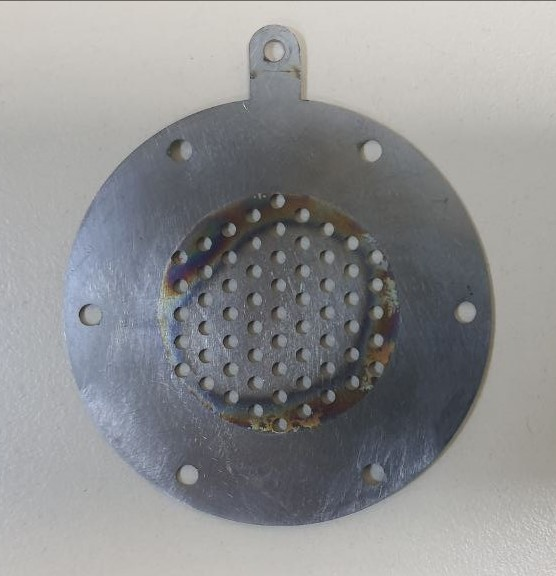
\includegraphics[width=0.4\linewidth]{fig/deneme4/test4_screen_after.jpg}
    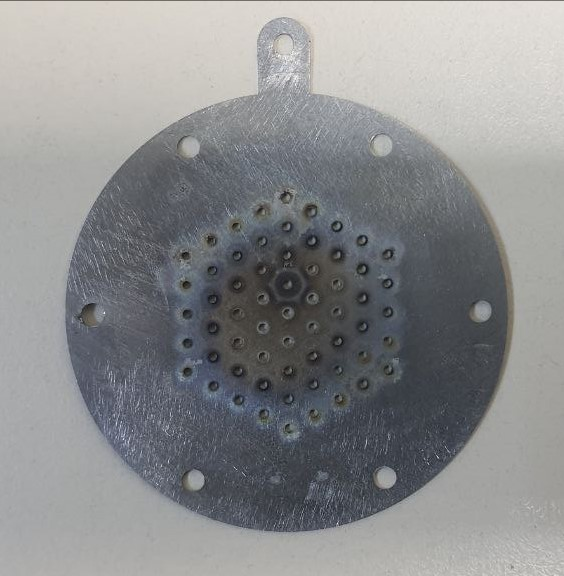
\includegraphics[width=0.4\linewidth]{fig/deneme4/test4_accel_after.jpg}
    \caption{Screen(\textit{left}) and acceleration(\textit{right}) grids after in fourth firing test}
    \label{fig:4th_grideg}
\end{figure}



% \section{Quoting}

% Generally, quoting is done by remaining faithful to the original text in terms of words, spelling and punctuation. In case there is a mistake, the correct version is written in square brackets in the quoted text.

% Short quotations (not longer than 40 words) must be given in quotation marks. Following the text quoted, the reference must be written and a full-stop must be placed afterwards.  

% Quotations longer than 40 words must not be shown in quotation  marks. Instead, they must be indented 1 tab space (1.27 cm) from the left side of the page. The font size for long quotations indented from the left must be 2 pt smaller than the font size used in main text body. However, it is not advised to quote very long texts and to quote very frequently. Unlike short quotations, references of long quotations must be placed after the full stop. (i.e., .(p.196))

% Example for a quotation at the beginning of a sentence;

% According to Jones (1998), "Students often had difficulty using APA style,  especially when it was their first time" (p. 199).

% Example for a quotation in the middle of a sentence;

% Interpreting these results, Robbins et al. (2003) suggested that the “therapists in dropout cases may have inadvertently validated parental negativity about the adolescent without adequately responding to the adolescent’s needs or concerns” (p. 541) contributing to an overall climate of negativity.

% Example for a quotation at the end of a sentence;

% Confusing this issue is the overlapping nature of roles in palliative care, whereby “medical needs are met by those in the medical disciplines; nonmedical needs may be addressed by anyone on the team” (Csikai \& Chaitin, 2006, p. 112). 

% Detailed information on quoting could be found on websites of Graduate Schools and associated links.

% \section{Footnotes}

% Footnotes could be used in theses to add content-expanding, content-enhancing, or additional information. 
% Footnote numbers must be placed directly after a quotation. In case the quotation is a paragraph, the footnote numbers must be placed directly after the last word of the paragraph (as superscript). In case the quotation is a concept or a noun, footnote numbers must be placed directly after that concept or noun (as superscript). 

% Footnote numbers in the main text body must be indicated as superscript, as shown\footnotemark. A punctuation mark must not be placed after the number.

% Footnotes must be written with a font size 2 pt smaller than the main text body font size.
 
% 1 space must be set between footnote line and footnote number, 1/2 space must be set between footnote number and the first line of the footnote. Footnotes must be separated from the main text body with a thin horizontal line. 

% Detailed information on footnotes could be found on the websites of Graduate Schools and associated links.

% \footnotetext{~Reference display can not be done with footnotes.~Footnotes could be used in theses to add content-expanding, content-enhancing, or additional information.~If these information must include references, these references must be indicated in References section.}

% \section{Second Level Title: First Letters Capital}

% \subsection{Third level title: Only first letter capital}


% \subsubsection{Fourth level title: Only first letter capital}



% \subsubsubsection{Fifth level title: No numbering after fourth level titles}



% % Include tilda to provide one letter spacing between the foot number and the text at the bottom - SBÖ
% \footnotetext{~~Footnotes must be written with a font size 2 pt smaller than the main text body font size.}

% \begin{figure}[t]
% 	\centering
% 	
\includegraphics[width=230pt,keepaspectratio=true]{./fig/sekil6}
% 	% sekil6.eps: 0x0 pixel, 300dpi, 0.00x0.00 cm, bb=14 14 555 489
% 	\caption{Example figure.}
% 	\label{Figure4.1}
% \end{figure}

% This indicates that the ANN is accurate at base flow and flow height values lower then 3 m. 

% \begin{table*}[h]
% 	{\setlength{\tabcolsep}{14pt}
% 		\caption{Example table.}
% 		\begin{center}
% 			\vspace{-6mm}
% 			\begin{tabular}{cccc}
% 				\hline \\[-2.45ex] \hline \\[-2.1ex]
% 				Column A & Column B & Column C & Column D \\
% 				\hline \\[-1.8ex]
% 				Row A & Row A & Row A & Row A \\
% 				Row B & Row B & Row B & Row B \\
% 				Row C & Row C & Row C & Row C \\
% 				[-0ex] \hline
% 			\end{tabular}
% 			\vspace{-6mm}
% 		\end{center}
% 		\label{Table4.1}}
% \end{table*}
